% !TeX TS-program = lualatex
% !TeX encoding = UTF-8
% TeX Live Version >=2022
% Diese Vorlage ist lizensiert unter GNU GENERAL PUBLIC LICENSE v3 (29 June 2007)
%
%% Anmerkungen %%
% Diese Vorlage wird weder von der HU-Berlin befürwortet, noch ist sie direkt mit ihr verbunden, autorisiert oder wird auf irgendeine Arte und Weise von ihr gesponsert. 
%
% Vor der Nutzung dieser Vorlage, sollte überprüft werden, ob sie noch den gültigen Richtlinien der HU-Berlin und des entsprechenden Studiengangs entspricht (Aktueller Stand: 2023-07-29 für MA(LIS) Bibliotheks- und Informationswissenschaft)
%
%% Dokumentkonfiguration %%
\directlua{pdf.setminorversion(7)} %Notwendig für korrekte Versionsanzeige wegen LuaLaTeX+pdfx Interaktion 
\documentclass[%
    fontsize=12pt,          %Schriftgröße festlegen
    a4paper,                %Seitenformat auf A4 setzen
    openright,              %Kapitel sollen auf der rechten Seite beginnen
    twoside=semi,           %Zweiseitiges Layout ohne abwechselnde Ränder
    headsepline,            %Trennlinie unterhalb des Headers hinzufügen
    titlepage=firstiscover, %\maketitle als Titelseite anzeigen
    numbers=noenddot,       %Nummerierung nach ISO 2145
    bibliography=totoc,     %Bibliographie zum Inhaltsverzeichnis hinzufügen
    listof=totoc,           %Abbildungs- und Tabellenverzeichnis im Inhaltsverzeichnis
    captions=tableheading,  %Setzt Formatierung für Tabellenüberschriften
    toc=index,              %Index zum Inhaltsverzeichnis hinzufügen
    hidelinks,				%Um Hyperlink-Boxen zu deaktivieren, falls Unterstrich gelöscht wird
    pdfa,                   %PDF/A Voreinstellungen
    %twocolumn,              %Für zweispaltige Darstellung
    %draft,                  %Auskommentieren für den Entwurfsmodus
    %final                   %Auskommentieren für den endgültigen Druck
    ]{scrbook}              %Verwendung der KOMA-Script book-Klasse

%% Dokumentpaketeausschluss
\PreventPackageFromLoading{fontenc,lmodern} %Sicherstellen dass Standardfonts nicht geladen werden

%% Dokumentpakete
%\usepackage{showframe}%Anzeige der Layout-Boxen
\usepackage{lipsum}   %Generierung von Dummy-Text
\usepackage[a-2b,mathxmp]{pdfx} %PDF/A-2b erzeugen
\usepackage[automark,draft=false]{scrlayer-scrpage} %Detaillierte Konfiguration von Kopf- und Fußzeilen
\usepackage[main=ngerman,british]{babel}%Sprache auf Deutsch setzen
\usepackage{fontspec}                   %LuaLaTeX Standard-Fontpackage
\usepackage{amsmath}                    %Erweiterte Mathematik
\usepackage{unicode-math}               %Unicode-Mathematikmodus erzwingen
    \setmainfont{TeX Gyre Termes}       %Allgemeine Schriftart setzen
    \setmathfont{TeX Gyre Termes Math}  %Mathematische Schriftart setzen
\usepackage{xcolor}   %Verbessertes Farbmanagement
\usepackage[%
    english=british,  %Anführungszeichen für Englisch auf britischen Stil setzen
    autostyle=true    %Anführungszeichen automatisch gemäß Sprache setzen
    ]{csquotes}       %Automatische Formatierung von Anführungszeichen
%\usepackage[%% DEKOMMENTIERE DIES FÜR AUTOR-JAHR ZITATE
    backend=biber,          %Backend auf biber setzen
    style=config/iso690_2021,   %Zitierstil (kompakt, Autor-Jahr) setzen
    bibnamessc=true,
    doi=true                %Fügt DOI zu Typen hinzu, die sonst keine anzeigen würden
    ]{biblatex}             %Verwendung der Bibliographie
    \AtBeginRefsection{\GenRefcontextData{sorting=ynt}} %Sortierung für Bibliographie festlegen
    \AtEveryCite{\localrefcontext[sorting=ynt]} %Sortierung für Verweise festlegen
    % Anmerkung: Einzeleinstellung notwendig, da sonst Bibliografie nach Jahr sortiert
 %Dekommentiere diese Linie für Autor-Jahr Zitate
\usepackage[backend=biber, style=config/iso690-numeric_2021, sorting=none, sortcites=true, bibnamessc=true, abbreviate=false, doi=true]{biblatex}
 %Dekommentiere diese Linie für numerische Zitate
\usepackage[%
    nameinlink, %Präfix in den Verlinkungen der Referenzen anzeigen
    ngerman,    %Sprache auf Deutsch setzen; unabhängig von Babel erforderlich
    capitalise, %Erster Buchstabe groß (nur wichtig für Englisch)
    noabbrev,   %Deaktiviert Abkürzungen wie Abb. für Abbildung
    ]{cleveref} %Automatische Präfix-Referenzierung
\usepackage[usetransparent=true]{svg} %Erlaubt Inkludierung von SVG Dateien
\usepackage{setspace}                  %Zeilenabstand festlegen
\usepackage{caption}                   %Anpassung der Beschriftungsformatierung
    %\captionsetup[table]{skip=10pt}    %Abstand zwischen Tabelle und Unterschrift
    \captionsetup{labelfont=bf} %Unterschrift in Fettschrift setzen
\usepackage{booktabs} %Bessere Tabellenästhetik
\usepackage{tabularx} %Tabellen mit Zeilenumbruch
\usepackage{array}    %Tabellenfeineinstellungen
\usepackage{multirow} %Tabellenzeilen kombinieren
\usepackage{multicol} %Mehrspaltige Dokumentdarstellung
\usepackage{adjustbox}%Bessere Version von \resizebox
\usepackage{glossaries-extra}%Abkürzung- und Begriffverwaltung
\usepackage{siunitx}  %Bessere Einheitenimplementation
\usepackage{pgfplots} %Akademische Diagramme
    \pgfplotsset{compat=1.18}
\usepackage{tikz}     %Erweiterte Zeichnungs- und Grafikkapazitäten
\usepackage{pdfpages} %Einbinden von PDF-Dateien

%% Neue Befehle und Variabeln
\DeclareNameFormat{labelname:poss}{% Based on labelname from biblatex.def
  \nameparts{#1}% Not needed if using Biblatex 3.4
  \ifcase\value{uniquename}%
    \usebibmacro{name:family}{\namepartfamily}{\namepartgiven}{\namepartprefix}{\namepartsuffix}%
  \or
    \ifuseprefix
      {\usebibmacro{name:given-family}{\namepartfamily}{\namepartgiveni}{\namepartprefix}{\namepartsuffixi}}
      {\usebibmacro{name:given-family}{\namepartfamily}{\namepartgiveni}{\namepartprefixi}{\namepartsuffixi}}%
  \or
    \usebibmacro{name:given-family}{\namepartfamily}{\namepartgiven}{\namepartprefix}{\namepartsuffix}%
  \fi
  \usebibmacro{name:andothers}%
  \ifnumequal{\value{listcount}}{\value{liststop}}{'s}{}}
\DeclareFieldFormat{shorthand:poss}{%
  \ifnameundef{labelname}{#1's}{#1}}
\DeclareFieldFormat{citetitle:poss}{\mkbibemph{#1}'s}
\DeclareFieldFormat{label:poss}{#1's}
\newrobustcmd*{\posscitealias}{%
  \AtNextCite{%
    \DeclareNameAlias{labelname}{labelname:poss}%
    \DeclareFieldAlias{shorthand}{shorthand:poss}%
    \DeclareFieldAlias{citetitle}{citetitle:poss}%
    \DeclareFieldAlias{label}{label:poss}}}
\newrobustcmd*{\posscite}{%
  \posscitealias%
  \textcite}
\newrobustcmd*{\Posscite}{\bibsentence\posscite}
\newrobustcmd*{\posscites}{%
  \posscitealias%
  \textcites} %\posscite-Befehl für besitzanzeigende Zitate im Englischen einbinden
\newcommand{\programme}[1]{\def\programmevar{#1}}
\newcommand{\degreecontext}[1]{\def\degreecontextvar{#1}}
\newcommand{\degree}[1]{\def\degreevar{#1}}
\newcommand{\faculty}[1]{\def\facultyvar{#1}}
\newcommand{\institute}[1]{\def\institutevar{#1}}
\newcommand{\firstsupervisor}[1]{\def\firstsupervisorvar{#1}}
\newcommand{\secondsupervisor}[1]{\def\secondsupervisorvar{#1}}
\newcommand{\keywords}[1]{\def\keywordsvar{#1}}
\newcommand{\languagemetadata}[1]{\def\languagevar{#1}}
\makeatletter
\def\subjectvar{\@subject}
\def\authorvar{\@author}
\def\titlevar{\@title}
\def\subtitlevar{\@subtitle}
\makeatother

\makeatletter
\def\mkfilename#1{%
  \if\relax\detokenize\expandafter{#1}\relax\else#1/\fi}
\AddToHook{include/before}%
  {\IfFileExists{\mkfilename\CurrentFilePath\CurrentFile}{}
     {\GenericError{}{Error: File \mkfilename\CurrentFilePath\CurrentFile.tex not found!}{\@gobble}{}}}
\makeatother

%% Formatierung
\RedeclareSectionCommand[%
    afterindent=false,%Eliminiert Einzug des ersten Paragrafen
    beforeskip=0pt%Eliminiert vertikalen Einzug vor dem Titel
    ]{chapter}%Eliminiert vertikalen Einzug vor Kapitel
\makeatletter
\def\ifdraft{\ifdim\overfullrule>\z@
  \expandafter\@firstoftwo\else\expandafter\@secondoftwo\fi}
\makeatother
\ifdraft{\usepackage{showframe}}{}%Fügt Layoutboxen zum Draft-Modus hinzu
\makeatletter
  \renewcommand{\@pnumwidth}{2em}
  \renewcommand{\@tocrmarg}{3em}
\makeatother %Mehr Platz für Figure-/Table-Nummerierung und Seitenangabe in Verzeichnissen
%% Change Link Colors
\def\tmp#1#2#3{%
  \definecolor{Hy#1color}{#2}{#3}%
  \hypersetup{#1color=Hy#1color}}
\tmp{link}{HTML}{800006}
\tmp{cite}{HTML}{2E7E2A}
\tmp{file}{HTML}{131877}
\tmp{url} {HTML}{8A0087}
\tmp{menu}{HTML}{727500}
\tmp{run} {HTML}{137776}
\def\tmp#1#2{%
  \colorlet{Hy#1bordercolor}{Hy#1color#2}%
  \hypersetup{#1bordercolor=Hy#1bordercolor}}
\tmp{link}{!60!white}
\tmp{cite}{!60!white}
\tmp{file}{!60!white}
\tmp{url} {!60!white}
\tmp{menu}{!60!white}
\tmp{run} {!60!white} %Bessere Standardfarben für Hyperlinks
\hypersetup{ pdfborderstyle={/W 1 /S /U} } %Unterstrichene Links die nicht gedruckt werden
%% This TeX-file sets most blank pages to contain an 'intentionally left blank' text
\newcommand*{\emptypageline}{THIS PAGE INTENTIONALLY LEFT BLANK}
\newcommand*{\blankpage}{%
  \par\vspace*{\fill}%
  {\centering\MakeUppercase{\emptypageline}\par}
  \vspace{\fill}%
}

\DeclareNewLayer[
    foreground,
    textarea,
    contents=\blankpage
  ]{blankpage.fg}
\DeclarePageStyleByLayers{blank}{blankpage.fg}
\KOMAoptions{cleardoublepage=blank} %Leere Seiten mit Absichtlich-Text
\renewcommand{\emptypageline}{Diese Seite wurde absichtlich leer gelassen} %Diesen Wert neu definieren, um die gewünschte Meldung anzuzeigen
\recalctypearea %Passt den Textbereich an Einstellungen an

%% Dokumentmetadaten %%
\subject{Publikationspraktiken von Forschungsdaten in Hochschulschriften}
\title{Publikationspraktiken für Forschungsdaten in Hochschulschriften}
\subtitle{Eine Untersuchung der Veröffentlichungsformate und -methoden}
\author{Dr. David Krassnig}
\date{14.06.2024}
\publishers{Verlag}
\dedication{Widmung}
\programme{Bibliotheks- und Informationswissenschaft im Fernstudium}
\degreecontext{im Rahmen des Weiterbildenden Masterstudiengangs}
\degree{Masterarbeit}
\faculty{Philosophische Fakultät}
\institute{Institut für Bibliotheks- und Informationswissenschaft}
\firstsupervisor{Dr. Sarah Dellmann}
\secondsupervisor{Prof. Dr. Robert Jäschke}
\keywords{Forschungsdatenmanagement, Bibliothekswissenschaft, TIB, Repositorium}
\languagemetadata{de-DE}
%
% PDF Metadaten
\pdfinfo{
  /Author (\authorvar)
  /Title (\titlevar: \subtitlevar)
  /Subject (\subjectvar)
  /Keywords (\keywordsvar)
  /Lang (\languagevar)
}


%% Bibliografie %%
\addbibresource{matter/backmatter/bibliography.bib} %Hauptbibliographieinformationen hinzufügen
%Anmerkung: Das Bibliografieformat muss oben unter Dokumentpakete eingestellt werden

%% Hauptdokument %%
%\includeonly{content/einfuehrung} %Selektive Dokumentgenerierung
\begin{document}
    %% Vorderer Teil
    \frontmatter
        %\makeatletter
\begin{titlepage}
\newgeometry{top=42.5mm,bottom=42.5mm,left=30mm,right=30mm}
\doublespacing\centering%
\textbf{\Huge\sffamily \@title}\vskip 2.5mm

\textbf{\Large\sffamily \@subtitle}\vfill

{\large eingereicht von}\\
\resizebox{%
      \ifdim\width>\textwidth
        \textwidth
      \else
        \width
      \fi
    }{!}{%
    \textbf{\Large\sffamily \@author}}\vfill

{\large als}\\
    \textbf{\Large\sffamily\degreevar}\vfill

{\large\degreecontextvar}\\
\resizebox{%
      \ifdim\width>\textwidth
        \textwidth
      \else
        \width
      \fi
    }{!}{%
    \textbf{\Large\sffamily\programmevar}}\vfill

{\large an der}\\
\textbf{\Large\sffamily Humboldt-Universität zu Berlin}\vfill

\resizebox{%
      \ifdim\width>\textwidth
        \textwidth
      \else
        \width
      \fi
    }{!}{%
    \textbf{\Large\sffamily\facultyvar}}

\resizebox{%
      \ifdim\width>\textwidth
        \textwidth
      \else
        \width
      \fi
    }{!}{%
    \textbf{\Large\sffamily\institutevar}}\vfill

\parbox{0cm}{\large%
    \begin{tabbing}
        \textbf{\sffamily1. Gutachter/in:} \= \firstsupervisorvar\\
        \textbf{\sffamily2. Gutachter/in:} \> \secondsupervisorvar
    \end{tabbing}
}\vfill


\textbf{\large\sffamily Berlin, \@date}
\end{titlepage}
\makeatother
\thispagestyle{empty}
\hbox{}\vfill\enlargethispage{15mm}
\begin{tabbing}
\noindent\textbf{Autor:}~~~~~\=Dr. David Krassnig\\
\>\orcidlink{0000-0002-1626-7987} \url{https://orcid.org/0000-0002-1626-7987}\\[\baselineskip]
\textbf{Lizenz (Dokument):}~~~~~\= \href{https://creativecommons.org/licenses/by/4.0/deed.de}{CC BY 4.0}\\
\textbf{DOI (Dokument):}\> \href{https://www.doi.org/10.5281/zenodo.11506621}{10.5281/zenodo.11506621}\\[.5\baselineskip]
\textbf{Lizenz (Daten):}\> \href{https://creativecommons.org/publicdomain/zero/1.0/deed.de}{CC0 1.0}\\
\textbf{DOI (Daten):}\> \href{https://www.doi.org/10.5281/zenodo.11401021}{10.5281/zenodo.11401021}
\end{tabbing}\newpage
\thispagestyle{empty}
\hbox{}
\vspace{30mm}
\begin{flushright}
{\LARGE\scshape Wasing the always of wanting of knowing}\\[.5\baselineskip]
{\footnotesize --Brandon Sanderson, \textit{Shadows of Self}}
\end{flushright}
\vfill
\hbox{}
\enlargethispage{30mm}
\vfill
\begin{figure}[b]
  \centering
\resizebox{22.5mm}{!}{
\begin{tikzpicture}[y=1mm, x=1mm, yscale=\globalscale,xscale=\globalscale, every node/.append style={scale=\globalscale}, inner sep=0pt, outer sep=0pt]
  \path[fill=c125b85,line width=3.175mm] (17.2619, 60.3734) -- (72.963, 95.5279)
   -- (14.8698, 131.9794) -- (72.963, 168.4314) -- (0.4748, 212.6876).. controls
   (0.3032, 187.8857) and (0.4119, 163.0838) .. (0.7807, 138.2818).. controls 
  (1.2623, 105.754) and (2.8937, 80.3161) .. (17.2619, 60.3734) -- cycle;



  \begin{scope}[fill=black,line width=1.7639mm,shift={(-4.758, 4.9148)}]
    \path[fill=black,line width=1.7639mm,miter limit=10.0] (74.0056, 74.9494).. 
  controls (74.2329, 73.9757) and (73.6718, 73.0178) .. (72.8205, 72.6021).. 
  controls (73.5744, 70.4553) and (75.9458, 71.7565) .. (74.9117, 73.6449).. 
  controls (74.7565, 74.1529) and (74.4414, 74.6695) .. (74.0056, 74.9494) -- 
  cycle(138.4185, 74.9038).. controls (138.3843, 74.9089) and (138.3086, 
  74.8922) .. (138.1743, 74.8452).. controls (137.6007, 74.7266) and (137.0486, 
  74.5335) .. (136.5009, 74.3254).. controls (135.8172, 74.4105) and (135.13, 
  74.4756) .. (134.4406, 74.4572).. controls (130.5626, 73.9996) and (126.4593, 
  72.6845) .. (122.5305, 73.9911).. controls (118.7325, 74.8439) and (113.9174, 
  74.5883) .. (111.4755, 71.1197).. controls (109.4837, 68.242) and (110.6627, 
  63.5553) .. (114.1636, 62.4728).. controls (118.9665, 60.8081) and (124.1583, 
  61.7104) .. (129.0949, 61.8911).. controls (136.5177, 62.36) and (143.9012, 
  64.0507) .. (151.3688, 63.8412).. controls (153.5412, 63.7184) and (156.4181, 
  62.2849) .. (155.8908, 59.6963).. controls (155.2096, 56.6484) and (151.4638, 
  56.0864) .. (148.8332, 56.0619).. controls (141.7311, 55.9693) and (135.0431, 
  59.0436) .. (128.0021, 59.3772).. controls (123.0159, 59.8684) and (117.9668, 
  59.5715) .. (113.1831, 57.9176).. controls (109.8742, 57.1998) and (105.6619, 
  56.2265) .. (102.8823, 58.795).. controls (101.9401, 59.7317) and (101.389, 
  61.033) .. (101.3001, 62.3528).. controls (101.8535, 63.5068) and (103.7288, 
  62.0123) .. (104.1982, 62.6887).. controls (102.5133, 63.0692) and (101.3809, 
  65.0022) .. (101.6962, 66.6313).. controls (101.9198, 66.7757) and (103.8952, 
  67.2426) .. (102.9333, 67.1798).. controls (101.3528, 66.9067) and (100.6688, 
  68.5328) .. (100.4786, 69.8022).. controls (100.2812, 70.2045) and (99.9983, 
  70.5249) .. (99.6658, 70.7974).. controls (99.8891, 71.7156) and (99.6631, 
  73.0456) .. (98.4427, 72.8674).. controls (97.8443, 72.8358) and (97.2591, 
  72.6874) .. (96.6972, 72.4789).. controls (96.8627, 73.2092) and (96.7223, 
  73.8282) .. (95.6028, 73.9635).. controls (95.0811, 73.8833) and (94.4796, 
  73.6944) .. (94.2029, 73.3145).. controls (92.9605, 73.5818) and (91.6884, 
  73.7351) .. (90.4339, 73.7714).. controls (88.9244, 73.9462) and (88.1105, 
  72.24) .. (86.5679, 72.4881).. controls (84.5808, 72.2535) and (82.6912, 
  71.2433) .. (80.7675, 71.0263).. controls (80.7304, 70.0931) and (81.5326, 
  69.4345) .. (81.0431, 68.5076).. controls (80.8135, 66.0916) and (84.0186, 
  64.4543) .. (86.0123, 65.7267).. controls (87.5081, 66.3458) and (89.1125, 
  65.9124) .. (90.2435, 64.9253).. controls (90.1591, 64.8692) and (90.0886, 
  64.8242) .. (89.9749, 64.7468).. controls (90.5772, 63.5638) and (90.7743, 
  62.1817) .. (90.6624, 60.8303).. controls (89.7975, 61.859) and (87.9907, 
  62.5602) .. (86.5788, 62.5721).. controls (84.2263, 62.5931) and (81.876, 
  60.2002) .. (79.6595, 61.985).. controls (79.2217, 62.3436) and (80.1238, 
  61.0665) .. (80.5059, 61.0522).. controls (83.0929, 59.9711) and (85.3784, 
  62.8581) .. (88.028, 61.9345).. controls (88.9719, 61.7392) and (89.8665, 
  61.3358) .. (90.6597, 60.7907).. controls (90.5829, 59.9119) and (90.3766, 
  59.0469) .. (90.0617, 58.2594).. controls (90.1279, 58.1517) and (90.2013, 
  58.0609) .. (90.2798, 57.9833).. controls (89.925, 57.7772) and (89.4985, 
  57.6738) .. (88.9895, 57.725).. controls (88.5118, 57.6285) and (87.2999, 
  57.715) .. (87.2109, 57.617).. controls (87.7928, 55.8173) and (85.4092, 
  54.9567) .. (84.0502, 54.573).. controls (83.9241, 54.5516) and (83.8003, 
  54.5238) .. (83.678, 54.4927).. controls (79.2098, 56.9291) and (74.817, 
  60.3467) .. (73.4119, 65.4001).. controls (73.1895, 66.7038) and (74.1887, 
  67.7711) .. (74.279, 69.0372).. controls (74.6129, 69.4838) and (75.6252, 
  69.8849) .. (75.2069, 70.5727).. controls (73.9268, 70.3314) and (72.7238, 
  71.5249) .. (72.3316, 72.6281).. controls (71.7672, 71.6998) and (72.1217, 
  71.1474) .. (72.1379, 70.1658).. controls (72.7389, 69.016) and (71.9384, 
  66.7239) .. (70.4184, 67.78).. controls (69.2478, 68.3949) and (68.697, 
  69.8618) .. (69.3088, 71.0334).. controls (69.233, 71.613) and (68.7003, 
  72.0389) .. (68.5475, 71.232).. controls (67.8815, 70.281) and (66.437, 
  70.0516) .. (65.5073, 70.3199).. controls (65.7173, 69.4283) and (67.041, 
  69.5708) .. (67.14, 68.5087).. controls (67.8283, 67.4293) and (70.2038, 
  66.8508) .. (69.2914, 65.2281).. controls (68.6504, 63.7411) and (66.4334, 
  64.0436) .. (66.1449, 65.5976).. controls (65.5926, 66.4667) and (65.7495, 
  65.7654) .. (65.7808, 65.1424).. controls (65.7808, 64.7539) and (65.6213, 
  64.4196) .. (65.3852, 64.1385).. controls (65.8082, 64.9784) and (65.1492, 
  66.4714) .. (63.9061, 66.0946).. controls (63.1079, 66.1297) and (61.8943, 
  65.3745) .. (61.8898, 64.8206).. controls (62.945, 65.1268) and (63.8034, 
  64.4045) .. (64.357, 63.6041).. controls (64.5576, 63.595) and (64.7284, 
  63.6237) .. (64.8741, 63.679).. controls (64.5416, 63.441) and (64.1805, 
  63.2658) .. (63.9018, 63.1608).. controls (64.565, 62.6878) and (65.3903, 
  62.9028) .. (65.834, 62.0685).. controls (66.9846, 61.506) and (68.4979, 
  61.9892) .. (69.522, 60.9703).. controls (71.0032, 60.1516) and (71.8134, 
  57.4413) .. (69.8937, 56.6734).. controls (69.8813, 56.6273) and (69.8689, 
  56.5596) .. (69.8568, 56.5036).. controls (69.2476, 56.5988) and (68.5632, 
  56.4872) .. (67.9528, 56.6718) -- (67.9745, 56.5655).. controls (68.085, 
  55.669) and (68.9844, 55.2451) .. (69.6137, 55.4867).. controls (69.5483, 
  55.2917) and (69.4684, 55.1153) .. (69.3614, 54.9962).. controls (71.2478, 
  54.0295) and (74.2586, 54.1003) .. (75.0826, 51.7406).. controls (75.1792, 
  49.9794) and (72.7743, 50.4729) .. (71.9551, 49.548).. controls (74.5725, 
  49.7791) and (77.0316, 48.5921) .. (78.7919, 46.7297).. controls (78.6297, 
  45.8029) and (79.0377, 44.7653) .. (78.7582, 43.8186).. controls (78.952, 
  42.6942) and (79.2938, 41.6152) .. (78.8109, 40.5082).. controls (79.1498, 
  39.3746) and (77.7144, 38.9032) .. (77.2574, 39.9618).. controls (76.7621, 
  40.9221) and (76.1942, 41.8346) .. (75.6648, 42.7503).. controls (75.912, 
  43.3265) and (75.5439, 44.5601) .. (74.9839, 43.5739).. controls (74.2948, 
  43.0379) and (73.1036, 43.1904) .. (72.5226, 43.2771).. controls (72.9522, 
  42.5064) and (73.4178, 42.3717) .. (74.2118, 41.8078).. controls (75.3028, 
  41.4399) and (75.7883, 39.5358) .. (74.317, 39.385).. controls (73.2887, 
  39.0696) and (72.9467, 40.535) .. (72.1227, 40.4116).. controls (72.6767, 
  39.4277) and (72.0353, 38.0857) .. (71.3842, 37.5255).. controls (72.0542, 
  37.4802) and (72.63, 38.1902) .. (73.3295, 37.6118).. controls (74.3819, 
  37.444) and (76.1444, 38.2914) .. (76.3751, 36.652).. controls (76.6819, 
  35.3956) and (74.5883, 35.4239) .. (74.3279, 34.9791).. controls (75.4526, 
  35.0425) and (76.3525, 33.9814) .. (76.2997, 32.8944).. controls (76.7551, 
  33.4485) and (76.9351, 34.0658) .. (77.7501, 34.2092).. controls (78.6288, 
  35.2352) and (80.7696, 35.4451) .. (80.882, 33.7029).. controls (80.7611, 
  33.4092) and (80.8172, 33.1493) .. (80.9292, 32.902).. controls (80.5987, 
  32.4921) and (79.9305, 31.8648) .. (79.7902, 31.6171).. controls (80.468, 
  31.2832) and (81.2426, 31.7642) .. (81.2086, 32.3876).. controls (81.3234, 
  32.1836) and (81.4208, 31.9794) .. (81.4229, 31.762).. controls (82.754, 
  32.5406) and (84.7111, 34.6164) .. (86.2505, 33.1315).. controls (86.7676, 
  32.5599) and (85.8794, 31.5966) .. (86.0519, 31.2731).. controls (88.6368, 
  34.1002) and (92.8614, 33.1787) .. (96.2072, 32.7924).. controls (97.3351, 
  32.5081) and (97.6354, 33.7209) .. (97.0336, 34.4739).. controls (96.7076, 
  35.6775) and (95.8937, 37.5679) .. (97.1296, 38.3872).. controls (99.4923, 
  37.4691) and (102.3162, 37.7796) .. (104.3468, 39.4018).. controls (108.5894, 
  42.3359) and (110.9891, 47.7208) .. (116.0936, 49.3874).. controls (117.0296, 
  49.6407) and (117.9604, 49.6686) .. (118.875, 49.5491).. controls (117.6105, 
  49.0637) and (116.658, 47.9003) .. (115.6899, 46.975).. controls (115.0442, 
  46.1616) and (115.9453, 46.6526) .. (116.2906, 46.899).. controls (117.8985, 
  47.8209) and (119.9299, 48.2341) .. (121.5766, 48.6532).. controls (121.5703, 
  48.7096) and (121.5589, 48.7633) .. (121.544, 48.8149).. controls (121.7604, 
  48.7278) and (121.9748, 48.6353) .. (122.1876, 48.5393).. controls (119.6257, 
  47.6886) and (117.161, 46.6053) .. (115.0399, 44.9082).. controls (113.1551, 
  43.1123) and (111.4327, 40.7568) .. (111.4685, 38.0426).. controls (111.1808, 
  37.0501) and (109.8385, 38.4124) .. (109.8727, 38.124).. controls (110.9981, 
  37.6035) and (110.4952, 36.2686) .. (109.3708, 36.3096).. controls (108.8912, 
  36.2842) and (108.2167, 34.8726) .. (108.877, 35.6856).. controls (109.7032, 
  36.4224) and (111.376, 36.561) .. (111.5222, 35.1902).. controls (112.2334, 
  33.9257) and (114.2083, 33.9914) .. (114.6997, 32.6899).. controls (114.5258, 
  30.7928) and (112.3978, 29.901) .. (111.3068, 28.5455).. controls (109.5652, 
  26.9572) and (106.8181, 25.1308) .. (104.5606, 26.8509).. controls (103.678, 
  27.6579) and (102.4196, 27.4456) .. (101.413, 27.8878).. controls (102.0712, 
  26.9718) and (101.391, 25.6269) .. (101.0049, 25.0007).. controls (101.6727, 
  25.0955) and (102.3512, 25.5096) .. (103.0522, 25.0587).. controls (104.1816, 
  25.237) and (105.7322, 23.4326) .. (104.2274, 22.8552).. controls (103.3527, 
  22.0638) and (102.6146, 20.7651) .. (101.2806, 20.8373).. controls (100.7037, 
  20.4819) and (100.8628, 20.2661) .. (101.4895, 20.2252).. controls (102.4576, 
  19.9281) and (103.0891, 18.8603) .. (103.2182, 18.0184).. controls (103.5438, 
  18.8956) and (103.8313, 19.9448) .. (104.9149, 20.2143).. controls (105.7605, 
  20.9608) and (106.3861, 23.1187) .. (107.852, 22.1851).. controls (108.3595, 
  20.6986) and (107.1809, 18.9579) .. (106.8509, 17.8519).. controls (107.743, 
  18.3388) and (108.9818, 17.828) .. (109.5352, 17.2951).. controls (109.1213, 
  18.1337) and (109.6103, 18.7439) .. (110.0143, 19.3901).. controls (110.3736, 
  20.9712) and (109.6521, 23.3766) .. (111.3475, 24.3164).. controls (112.1213, 
  24.7732) and (112.8505, 24.0479) .. (113.3361, 23.7472).. controls (114.1373, 
  24.0913) and (114.9697, 22.6761) .. (115.1744, 23.8715).. controls (116.065, 
  25.2345) and (115.9155, 27.3467) .. (117.3215, 28.3366).. controls (118.5545, 
  28.8235) and (118.8606, 27.0537) .. (119.2239, 26.5519).. controls (119.5312, 
  29.2178) and (121.6164, 31.2604) .. (124.0661, 32.1174).. controls (125.631, 
  32.7702) and (125.8475, 34.9839) .. (124.3064, 35.8066).. controls (123.5751, 
  36.2621) and (121.7086, 36.3476) .. (122.3395, 37.6514).. controls (124.5447, 
  39.801) and (126.0031, 42.5489) .. (127.287, 45.3043).. controls (127.4764, 
  45.6914) and (127.676, 46.0779) .. (127.8892, 46.4568).. controls (130.4484, 
  46.0439) and (133.1025, 46.2672) .. (135.5882, 47.0802).. controls (137.1431, 
  47.5067) and (138.9095, 46.7277) .. (139.4141, 45.2072).. controls (139.2962, 
  45.2396) and (139.1496, 45.1759) .. (138.9904, 44.9152).. controls (139.2755, 
  44.6021) and (139.46, 44.5136) .. (139.5666, 44.5398).. controls (140.0837, 
  42.5111) and (139.2282, 39.5601) .. (136.7575, 39.5831).. controls (135.3558, 
  39.555) and (134.1255, 40.8601) .. (132.7037, 40.0796).. controls (131.9323, 
  40.3547) and (131.8489, 40.1208) .. (132.3755, 39.5907).. controls (132.8763, 
  38.867) and (132.7887, 37.8143) .. (132.3223, 37.1604).. controls (132.9538, 
  37.3226) and (133.472, 38.0107) .. (134.2437, 37.5863).. controls (135.2, 
  37.3062) and (135.4766, 36.1703) .. (134.5936, 35.5407).. controls (134.1334, 
  34.6401) and (133.2272, 34.3481) .. (132.3538, 34.1158).. controls (133.6573, 
  34.0536) and (134.6748, 32.8375) .. (134.5698, 31.6144).. controls (135.3636, 
  32.1693) and (134.9443, 33.5241) .. (135.9268, 34.0523).. controls (136.7079, 
  34.5089) and (137.6611, 35.1945) .. (138.1846, 34.1413).. controls (138.0666, 
  35.1748) and (138.7021, 33.5672) .. (138.0712, 33.5602).. controls (138.8896, 
  33.5713) and (139.675, 32.9868) .. (139.8938, 32.2547).. controls (142.3734, 
  32.4057) and (143.1067, 35.4928) .. (142.5276, 37.5103).. controls (142.3974, 
  38.5992) and (143.3595, 39.3909) .. (144.1619, 39.7779).. controls (144.2489, 
  40.5173) and (145.1052, 40.8986) .. (145.5672, 41.0709).. controls (144.543, 
  43.1405) and (144.2853, 45.6431) .. (145.5233, 47.6907).. controls (146.7109, 
  49.0505) and (145.6984, 51.6863) .. (143.698, 50.7998).. controls (141.8579, 
  49.8009) and (138.7648, 49.747) .. (138.0283, 52.1487).. controls (137.5931, 
  53.1951) and (136.1941, 53.9307) .. (136.0283, 54.853).. controls (136.452, 
  56.301) and (138.2401, 54.8087) .. (139.3072, 54.9219).. controls (144.433, 
  54.0942) and (149.9989, 53.1166) .. (154.8197, 55.6566).. controls (157.4227, 
  56.9065) and (158.5548, 60.4142) .. (156.9011, 62.8455).. controls (155.375, 
  65.2792) and (152.3527, 65.5903) .. (149.7686, 65.7712).. controls (148.2728, 
  66.1689) and (146.8723, 66.9253) .. (145.6454, 67.8499).. controls (145.8813, 
  67.011) and (146.4084, 65.2333) .. (144.915, 65.3762).. controls (143.1974, 
  65.3927) and (141.5988, 66.7267) .. (140.4266, 67.4983).. controls (140.2197, 
  66.6467) and (141.2775, 65.0462) .. (139.7929, 64.9649).. controls (138.0214, 
  64.9568) and (136.7284, 66.4754) .. (135.3316, 67.2189).. controls (135.2099, 
  66.3437) and (136.2233, 64.6453) .. (134.7244, 64.5401).. controls (132.9134, 
  64.6067) and (131.2049, 66.0433) .. (129.8638, 66.7072).. controls (130.1611, 
  65.745) and (130.5444, 63.762) .. (128.9202, 63.8938).. controls (127.0907, 
  63.9975) and (125.8248, 65.9156) .. (124.396, 66.4967).. controls (124.4531, 
  65.5576) and (125.2388, 63.5304) .. (123.5962, 63.5965).. controls (121.9143, 
  63.62) and (121.0497, 65.8) .. (119.9287, 66.291).. controls (119.7233, 
  64.4449) and (117.7417, 63.367) .. (116.0339, 63.9931).. controls (113.2404, 
  64.4618) and (111.007, 67.8989) .. (112.8841, 70.4132).. controls (115.3436, 
  73.6637) and (120.2369, 73.4121) .. (123.5755, 71.7887).. controls (125.7789, 
  70.3815) and (128.5143, 68.703) .. (131.1845, 70.0166).. controls (132.2171, 
  70.4477) and (133.2796, 71.047) .. (134.3674, 71.5619).. controls (134.762, 
  71.5478) and (135.4088, 71.6282) .. (135.7684, 71.5695).. controls (137.4107, 
  71.622) and (139.052, 70.8464) .. (140.6708, 71.2569).. controls (139.4596, 
  72.5904) and (137.853, 72.4762) .. (136.2307, 72.3042).. controls (137.537, 
  72.6988) and (138.8759, 72.7813) .. (140.2416, 72.1365).. controls (141.8216, 
  71.36) and (144.4393, 71.5895) .. (145.4853, 72.487).. controls (143.7679, 
  71.898) and (142.2303, 72.5825) .. (140.6724, 73.2619).. controls (141.9807, 
  73.2138) and (143.292, 73.3539) .. (144.4175, 74.187).. controls (143.1274, 
  73.6293) and (141.6759, 73.6018) .. (140.3219, 73.4132).. controls (139.521, 
  73.7576) and (138.7098, 74.0697) .. (137.8628, 74.1892).. controls (137.88, 
  74.2299) and (137.8985, 74.2665) .. (137.9149, 74.3102).. controls (137.935, 
  74.4497) and (138.5665, 74.8814) .. (138.4184, 74.9038) -- cycle(65.7569, 
  73.4415).. controls (65.6539, 73.4463) and (65.5507, 73.4447) .. (65.4476, 
  73.4371).. controls (64.8503, 73.3987) and (64.2333, 73.145) .. (65.0488, 
  72.901).. controls (65.8818, 72.5711) and (65.8665, 71.496) .. (66.1118, 
  70.9553).. controls (67.0187, 70.8036) and (68.7166, 71.5291) .. (67.6794, 
  72.5565).. controls (67.1825, 73.0783) and (66.4778, 73.408) .. (65.7569, 
  73.4415) -- cycle(82.8489, 64.6187).. controls (82.8215, 64.6148) and 
  (82.7814, 64.5868) .. (82.7257, 64.5249).. controls (82.619, 63.492) and 
  (83.0404, 64.6461) .. (82.8489, 64.6187) -- cycle(82.8738, 58.7836).. controls
   (82.8282, 58.7803) and (82.8121, 58.7516) .. (82.8466, 58.6805).. controls 
  (82.9263, 58.033) and (82.1731, 57.4099) .. (83.2813, 57.7353).. controls 
  (83.6946, 57.1975) and (84.213, 58.1525) .. (84.8429, 58.0999).. controls 
  (84.3788, 58.2396) and (83.6721, 58.4572) .. (83.4771, 58.5845).. controls 
  (83.4088, 58.5738) and (83.0103, 58.7933) .. (82.8738, 58.7836) -- 
  cycle(84.8429, 58.0999).. controls (84.9308, 58.0735) and (85.012, 58.0486) ..
   (85.074, 58.0299).. controls (84.9954, 58.0695) and (84.9183, 58.0936) .. 
  (84.8429, 58.0999) -- cycle(85.074, 58.0299).. controls (85.0965, 58.0187) and
   (85.1187, 58.0112) .. (85.1413, 57.9968).. controls (85.3325, 57.951) and 
  (85.2459, 57.9782) .. (85.074, 58.0299) -- cycle(72.382, 45.9153).. controls 
  (72.2981, 45.92) and (72.2134, 45.919) .. (72.1286, 45.9121).. controls 
  (72.574, 45.5418) and (72.9826, 44.6419) .. (72.7309, 43.9164).. controls 
  (73.5565, 43.4545) and (74.9938, 44.3908) .. (73.936, 45.1622).. controls 
  (73.5275, 45.5794) and (72.9696, 45.8828) .. (72.382, 45.9153) -- 
  cycle(145.2579, 40.594).. controls (145.0875, 40.6016) and (144.8859, 40.5533)
   .. (144.6507, 40.4328).. controls (144.8163, 39.776) and (145.6369, 39.1161) 
  .. (145.8629, 38.7051).. controls (146.144, 39.4797) and (145.9961, 40.5606) 
  .. (145.2579, 40.594) -- cycle(70.8681, 40.13).. controls (69.9789, 40.1081) 
  and (68.9882, 39.3814) .. (68.8616, 38.5684).. controls (69.5351, 39.0149) and
   (70.3918, 38.7618) .. (70.962, 38.3774).. controls (71.3334, 38.8821) and 
  (72.0276, 40.1331) .. (70.8681, 40.13) -- cycle(131.3211, 39.5739).. controls 
  (130.2048, 39.2536) and (129.5362, 38.0869) .. (129.5598, 36.9623).. controls 
  (130.0011, 37.6921) and (130.9092, 37.7305) .. (131.5805, 37.6357).. controls 
  (132.1251, 38.0424) and (131.9422, 39.4215) .. (131.3211, 39.5739) -- 
  cycle(74.9572, 34.4631).. controls (74.8752, 34.4629) and (74.7923, 34.4559) 
  .. (74.7108, 34.4424).. controls (73.4688, 34.3234) and (73.6805, 32.03) .. 
  (74.3815, 31.6394).. controls (74.3523, 32.6168) and (75.3198, 33.0318) .. 
  (75.9339, 33.456).. controls (76.0726, 34.1404) and (75.5312, 34.4646) .. 
  (74.9572, 34.4631) -- cycle(132.4991, 33.4772).. controls (131.4508, 33.0383) 
  and (131.3899, 31.3819) .. (131.7731, 30.4223).. controls (132.1036, 31.2702) 
  and (133.1015, 31.7081) .. (133.7438, 32.0084).. controls (133.6472, 32.6398) 
  and (133.2599, 33.5145) .. (132.4991, 33.4772) -- cycle(138.0081, 32.8168).. 
  controls (137.2717, 32.5706) and (137.4882, 30.8696) .. (137.7754, 30.7734).. 
  controls (137.8911, 31.4635) and (138.6204, 31.8955) .. (139.0608, 32.1831).. 
  controls (138.9113, 32.6039) and (138.4385, 32.8452) .. (138.0081, 32.8168) --
   cycle(100.6304, 27.3583).. controls (99.7634, 27.324) and (98.6909, 26.804) 
  .. (98.4557, 26.0321).. controls (99.1152, 26.3901) and (100.0033, 26.1827) ..
   (100.4248, 25.6241).. controls (100.8975, 25.8845) and (101.2016, 27.1137) ..
   (100.6304, 27.3583) -- cycle(113.8059, 23.4434).. controls (113.2861, 
  23.1096) and (113.3104, 21.9849) .. (113.4456, 21.7423).. controls (114.5091, 
  22.1248) and (114.1572, 22.9059) .. (113.8059, 23.4434) -- cycle(101.2116, 
  20.0809).. controls (100.3749, 19.3186) and (100.1258, 17.7701) .. (100.619, 
  16.7004).. controls (100.8483, 17.5769) and (101.604, 18.4652) .. (102.5279, 
  18.4791).. controls (102.2617, 19.0862) and (101.9149, 19.9175) .. (101.2116, 
  20.0809) -- cycle(107.6544, 17.1448).. controls (106.6715, 17.052) and 
  (107.5212, 15.5369) .. (107.9192, 15.0933).. controls (108.2537, 14.746) and 
  (109.0055, 14.3685) .. (108.5627, 15.1052).. controls (108.2747, 15.8757) and 
  (109.3892, 16.7754) .. (108.2073, 17.0846).. controls (108.0289, 17.1386) and 
  (107.8401, 17.1567) .. (107.6544, 17.1448) -- cycle;



    \path[fill=black,line width=1.7639mm,miter limit=10.0] (133.9103, 
  227.7543).. controls (133.896, 227.7582) and (133.8673, 227.754) .. (133.8209,
   227.7393).. controls (133.1262, 227.6136) and (132.4655, 227.3664) .. 
  (131.8076, 227.1099).. controls (131.1918, 227.1839) and (130.5759, 227.237) 
  .. (129.9411, 227.2246).. controls (126.1714, 226.774) and (122.3305, 
  225.5747) .. (118.548, 226.6835).. controls (113.7528, 227.4472) and 
  (108.4247, 227.5979) .. (104.0429, 225.203).. controls (101.173, 223.7623) and
   (100.657, 219.4237) .. (103.1406, 217.3849).. controls (107.0503, 214.3737) 
  and (112.2106, 215.2806) .. (116.8313, 215.2119).. controls (126.4887, 
  215.2667) and (136.0111, 217.2186) .. (145.6662, 217.6464).. controls 
  (149.3454, 217.629) and (153.4501, 218.053) .. (156.7198, 216.031).. controls 
  (158.5323, 214.8459) and (157.8154, 211.928) .. (155.834, 211.3698).. controls
   (151.7653, 210.0862) and (147.3671, 210.9647) .. (143.2834, 211.7558).. 
  controls (135.7135, 213.8114) and (127.6936, 214.4066) .. (119.9298, 
  212.9888).. controls (112.7464, 212.1877) and (105.7056, 209.63) .. (98.4019, 
  210.1383).. controls (95.6838, 210.214) and (92.6525, 211.664) .. (92.1542, 
  214.5897).. controls (92.7709, 215.8417) and (94.0859, 214.2983) .. (95.0801, 
  214.9638).. controls (93.3865, 215.2621) and (92.2069, 217.175) .. (92.5335, 
  218.7951).. controls (92.8483, 218.9557) and (94.7721, 219.4172) .. (93.5427, 
  219.3083).. controls (92.0831, 219.1564) and (91.5745, 220.6975) .. (91.3729, 
  221.842).. controls (91.1895, 222.233) and (90.9217, 222.5437) .. (90.6044, 
  222.8063).. controls (90.8302, 223.7069) and (90.6624, 225.026) .. (89.4334, 
  224.8614).. controls (88.8633, 224.8325) and (88.3037, 224.6972) .. (87.7679, 
  224.4992).. controls (87.8858, 225.092) and (87.7732, 225.6161) .. (87.0377, 
  225.9131).. controls (86.9274, 225.9458) and (86.8103, 225.9465) .. (86.6967, 
  225.9363).. controls (86.1454, 225.8649) and (85.538, 225.6555) .. (85.2973, 
  225.2413).. controls (84.1148, 225.5006) and (82.9041, 225.6516) .. (81.7073, 
  225.6728).. controls (80.2529, 225.8332) and (79.4594, 224.2072) .. (77.9763, 
  224.4263).. controls (76.0629, 224.2126) and (74.3543, 223.1965) .. (72.4123, 
  223.0858).. controls (72.306, 222.1577) and (73.1763, 221.5037) .. (72.6841, 
  220.5899).. controls (72.443, 218.3116) and (75.4229, 216.7048) .. (77.338, 
  217.8443).. controls (78.7608, 218.4801) and (80.3546, 218.109) .. (81.4815, 
  217.1787).. controls (81.4512, 217.1516) and (81.4216, 217.1256) .. (81.3895, 
  217.094).. controls (82.389, 215.1788) and (82.3039, 212.707) .. (81.4773, 
  210.7486).. controls (81.5329, 210.6558) and (81.5938, 210.5752) .. (81.6587, 
  210.5047).. controls (81.304, 210.2753) and (80.8692, 210.1545) .. (80.3405, 
  210.2003).. controls (79.8879, 210.056) and (78.3462, 210.2718) .. (78.615, 
  210.0763).. controls (79.1575, 208.3217) and (76.8271, 207.4265) .. (75.4565, 
  207.1571).. controls (74.9816, 207.1374) and (74.5855, 206.9894) .. (74.2323, 
  206.77).. controls (69.8444, 209.0888) and (65.3764, 212.4088) .. (64.0918, 
  217.403).. controls (63.9973, 218.5812) and (64.8356, 219.5597) .. (64.9357, 
  220.7129).. controls (65.2389, 221.0282) and (66.3043, 221.6709) .. (65.7527, 
  222.0993).. controls (64.5707, 221.9078) and (63.4532, 223.1127) .. (63.0991, 
  224.0315).. controls (62.5659, 223.035) and (62.961, 222.2692) .. (63.0676, 
  221.1387).. controls (63.4027, 220.0845) and (62.4071, 218.6786) .. (61.3189, 
  219.5258).. controls (60.2219, 220.1064) and (59.7051, 221.4798) .. (60.2781, 
  222.5804).. controls (60.2103, 223.1044) and (59.7251, 223.5006) .. (59.5748, 
  222.7773).. controls (58.9899, 221.8186) and (57.4683, 221.7738) .. (56.7538, 
  221.8616).. controls (57.0308, 221.1038) and (58.1698, 221.193) .. (58.2746, 
  220.2245).. controls (58.9208, 219.2118) and (61.16, 218.6469) .. (60.2885, 
  217.1296).. controls (59.5608, 215.5616) and (57.4586, 216.227) .. (57.1703, 
  217.7275).. controls (56.6128, 218.291) and (57.2727, 216.8579) .. (56.8577, 
  216.5203).. controls (56.8029, 216.3244) and (56.692, 216.1573) .. (56.5528, 
  216.0113).. controls (57.0715, 216.7712) and (56.4442, 218.3203) .. (55.2293, 
  217.9554).. controls (54.4869, 217.997) and (53.3274, 217.2587) .. (53.3535, 
  216.7498).. controls (54.3428, 217.0382) and (55.1529, 216.3671) .. (55.6701, 
  215.6129).. controls (55.8669, 215.6077) and (56.0328, 215.6409) .. (56.1724, 
  215.7008).. controls (55.8323, 215.4753) and (55.4536, 215.3185) .. (55.2257, 
  215.1917).. controls (55.8406, 214.7442) and (56.6164, 214.9606) .. (57.0328, 
  214.183).. controls (58.1169, 213.6496) and (59.5428, 214.11) .. (60.5081, 
  213.1521).. controls (61.8894, 212.3833) and (62.6835, 209.8432) .. (60.8677, 
  209.126).. controls (60.8558, 209.0808) and (60.8452, 209.0171) .. (60.8342, 
  208.9632).. controls (60.2599, 209.0538) and (59.572, 208.9591) .. (59.0622, 
  209.0402).. controls (59.1533, 208.232) and (60.0126, 207.7867) .. (60.6047, 
  208.0015).. controls (60.5435, 207.8356) and (60.4668, 207.6846) .. (60.3598, 
  207.5762).. controls (62.1393, 206.6716) and (65.107, 206.7161) .. (65.7388, 
  204.4182).. controls (65.6903, 202.8616) and (63.6078, 203.3186) .. (62.8004, 
  202.4664).. controls (66.0873, 202.7681) and (69.1109, 200.6644) .. (70.6573, 
  197.8667).. controls (70.6976, 197.9184) and (70.74, 197.969) .. (70.7814, 
  198.0202).. controls (70.7859, 197.3544) and (70.8326, 196.6917) .. (71.0619, 
  196.0332).. controls (70.6116, 195.0974) and (71.2059, 193.4103) .. (69.7003, 
  193.4975).. controls (66.3343, 193.049) and (62.758, 192.7292) .. (59.4668, 
  193.7104).. controls (58.4581, 194.2942) and (58.2846, 195.5895) .. (57.3904, 
  196.3045).. controls (57.1639, 196.8361) and (57.5835, 197.818) .. (56.7734, 
  197.9814).. controls (56.2293, 196.8159) and (54.5123, 196.7818) .. (53.5886, 
  196.9743).. controls (54.1492, 195.477) and (56.3738, 195.6322) .. (56.9155, 
  193.9734).. controls (56.8863, 192.4447) and (54.2976, 192.1975) .. (53.4532, 
  193.2815).. controls (53.4463, 193.9445) and (51.8371, 194.3604) .. (52.4812, 
  193.4546).. controls (52.8867, 192.3797) and (51.9758, 191.1178) .. (51.4327, 
  190.6113).. controls (52.2239, 190.2909) and (52.837, 191.3149) .. (53.6796, 
  190.7927).. controls (54.8801, 190.6838) and (56.6803, 192.1338) .. (57.3739, 
  190.5286).. controls (58.1097, 189.1994) and (56.616, 187.7367) .. (55.2944, 
  188.3934).. controls (54.348, 188.4797) and (54.9234, 188.1885) .. (55.4055, 
  187.8523).. controls (55.6951, 187.6383) and (55.845, 187.3326) .. (55.9151, 
  187.0007).. controls (55.6939, 187.513) and (55.0018, 187.8559) .. (54.402, 
  187.8575).. controls (53.2873, 187.401) and (52.7552, 185.4916) .. (53.3788, 
  184.8117).. controls (53.7471, 185.8114) and (54.8127, 186.0624) .. (55.7559, 
  186.0271).. controls (55.8684, 186.1807) and (55.932, 186.3293) .. (55.9637, 
  186.472).. controls (55.9637, 186.0246) and (55.8799, 185.5879) .. (55.8272, 
  185.3067).. controls (56.5631, 185.538) and (56.8901, 186.263) .. (57.7692, 
  186.1237).. controls (58.8474, 186.6485) and (59.3263, 188.0679) .. (60.6709, 
  188.243).. controls (62.1798, 188.8638) and (64.3656, 187.9783) .. (64.2676, 
  186.2209).. controls (64.2765, 186.2163) and (64.2845, 186.2103) .. (64.2932, 
  186.2054).. controls (63.8847, 185.7509) and (63.6429, 185.0166) .. (63.0907, 
  184.729).. controls (63.8378, 184.3116) and (64.6954, 184.7303) .. (64.857, 
  185.3605).. controls (64.9299, 185.1276) and (64.9785, 184.9024) .. (65.0348, 
  184.7533).. controls (66.854, 185.5784) and (68.6072, 187.9645) .. (70.8231, 
  187.0849).. controls (72.1315, 186.2902) and (70.5527, 184.9911) .. (70.9016, 
  183.9399).. controls (74.4396, 187.7919) and (80.3389, 187.4734) .. (84.9943, 
  186.3113).. controls (85.8181, 185.8328) and (87.8064, 186.0829) .. (87.0515, 
  187.4446).. controls (86.7458, 188.4763) and (86.0741, 189.8227) .. (86.543, 
  190.7937).. controls (87.465, 191.4282) and (88.6444, 190.2445) .. (89.7227, 
  190.4423).. controls (96.791, 189.8911) and (102.6004, 194.6594) .. (107.8337,
   198.755).. controls (111.6071, 201.8461) and (116.1865, 204.7564) .. 
  (121.1931, 204.7061).. controls (121.1519, 204.6588) and (121.1114, 204.6141) 
  .. (121.0696, 204.5645).. controls (120.8971, 204.4133) and (120.7248, 
  204.2619) .. (120.5523, 204.1108).. controls (119.939, 203.5683) and 
  (118.7353, 202.7961) .. (118.769, 202.0101).. controls (119.9547, 202.7436) 
  and (121.2312, 203.3395) .. (122.56, 203.7718).. controls (121.7436, 202.6143)
   and (121.6897, 201.1183) .. (121.3301, 199.8159).. controls (120.8129, 
  199.142) and (120.1179, 200.3938) .. (119.8258, 200.2448).. controls 
  (120.6554, 199.8186) and (120.6315, 198.0957) .. (119.4093, 198.5566).. 
  controls (118.9422, 198.641) and (118.112, 198.1112) .. (118.122, 197.9571).. 
  controls (119.4308, 198.9467) and (121.4708, 198.1993) .. (121.9031, 
  196.6161).. controls (123.914, 194.1342) and (127.4177, 194.2215) .. 
  (130.2174, 193.4453).. controls (130.9335, 192.1921) and (128.8909, 191.8202) 
  .. (128.0284, 191.7709).. controls (124.7865, 191.6666) and (121.2971, 
  191.176) .. (118.2434, 192.5228).. controls (116.2903, 193.3613) and 
  (117.0543, 195.8731) .. (115.6384, 197.1127).. controls (115.5068, 197.5152) 
  and (115.281, 198.5098) .. (115.0421, 197.5825).. controls (114.6649, 
  196.7748) and (113.411, 196.5946) .. (112.9368, 196.3981).. controls 
  (113.4338, 195.9579) and (114.2036, 195.7678) .. (114.3429, 194.9568).. 
  controls (115.1444, 194.3233) and (115.0355, 192.1248) .. (113.6902, 
  192.6396).. controls (112.5206, 192.8282) and (111.0632, 192.3714) .. 
  (110.1959, 193.4163).. controls (109.5419, 193.5928) and (109.4695, 193.3565) 
  .. (109.8713, 192.8639).. controls (110.3258, 191.9776) and (109.9206, 190.82)
   .. (109.4579, 190.1705).. controls (110.2688, 190.4974) and (111.1923, 
  191.0463) .. (112.0789, 190.4341).. controls (113.1805, 190.2451) and 
  (115.1449, 191.3302) .. (115.4813, 189.6574).. controls (115.0371, 188.621) 
  and (113.9136, 188.5041) .. (112.9688, 188.4068).. controls (112.6489, 
  188.1058) and (111.2894, 188.3909) .. (112.234, 187.949).. controls (112.9893,
   187.4977) and (113.1238, 186.2427) .. (113.1202, 185.7191).. controls 
  (113.5387, 186.516) and (114.2808, 186.5189) .. (115.0255, 186.5816).. 
  controls (116.4713, 187.167) and (117.754, 189.3279) .. (119.4816, 188.52).. 
  controls (120.2389, 188.2309) and (120.0981, 187.2896) .. (120.2536, 
  186.8095).. controls (120.7036, 186.4705) and (120.9251, 185.8859) .. 
  (120.8768, 185.3321).. controls (122.9769, 185.5381) and (124.7555, 186.947) 
  .. (126.7917, 187.2586).. controls (128.3038, 187.0187) and (127.4854, 
  185.1939) .. (126.9819, 184.3848).. controls (126.907, 183.8429) and 
  (127.8661, 185.0891) .. (128.2309, 185.2096).. controls (131.0627, 187.5684) 
  and (135.233, 188.2403) .. (138.5848, 186.639).. controls (140.0176, 185.8801)
   and (142.3063, 187.3153) .. (141.4337, 188.9411).. controls (139.7764, 
  191.2405) and (136.9207, 192.5968) .. (135.8806, 195.3857).. controls 
  (135.5657, 196.1426) and (135.3177, 196.9539) .. (135.214, 197.7768).. 
  controls (136.1924, 197.2915) and (137.2192, 196.9044) .. (138.3244, 
  196.6776).. controls (141.911, 195.6758) and (145.7811, 196.1322) .. 
  (149.2632, 197.4037).. controls (152.4799, 198.2755) and (156.1659, 199.7972) 
  .. (159.3975, 198.229).. controls (161.215, 197.1917) and (161.1373, 193.5814)
   .. (158.9148, 193.1657).. controls (157.3619, 193.3596) and (155.7989, 
  194.2615) .. (154.2319, 193.5192).. controls (153.0225, 193.7871) and 
  (154.5895, 192.6445) .. (154.2764, 191.9482).. controls (154.3131, 191.4706) 
  and (153.5506, 190.2978) .. (154.3332, 190.9762).. controls (155.2575, 
  191.6826) and (157.4228, 190.9524) .. (156.9506, 189.7044).. controls 
  (156.2878, 188.7868) and (155.4852, 187.911) .. (154.3156, 187.796).. controls
   (155.6132, 187.7534) and (156.5691, 186.5337) .. (156.5119, 185.3605).. 
  controls (157.2132, 185.8024) and (156.9508, 186.9341) .. (157.839, 
  187.3066).. controls (158.6518, 188.1356) and (160.2394, 188.6805) .. 
  (160.8548, 187.9216).. controls (160.7427, 188.7257) and (161.3163, 187.2629) 
  .. (160.7447, 187.2374).. controls (161.5435, 187.2502) and (162.2771, 
  186.6442) .. (162.4934, 185.9599).. controls (164.9687, 186.1231) and 
  (165.6336, 189.2221) .. (165.0127, 191.2066).. controls (164.6647, 192.3024) 
  and (165.7896, 192.9296) .. (166.4725, 193.3445).. controls (166.621, 
  193.9408) and (167.4611, 194.1514) .. (167.7407, 194.4214).. controls 
  (166.6181, 196.8925) and (163.2626, 197.7281) .. (162.9446, 200.6862).. 
  controls (162.8296, 202.0183) and (163.8568, 204.1877) .. (162.2201, 
  204.9329).. controls (160.0583, 204.8417) and (158.3145, 203.1276) .. 
  (156.084, 203.2178).. controls (151.1383, 202.7054) and (145.9422, 204.0368) 
  .. (142.2585, 207.4914).. controls (141.6869, 208.3295) and (139.7481, 
  208.9496) .. (140.2312, 210.0107).. controls (140.8306, 210.962) and 
  (142.4308, 209.7062) .. (143.4501, 209.805).. controls (148.1431, 209.1308) 
  and (153.1483, 208.0609) .. (157.625, 210.0463).. controls (160.2368, 
  211.1402) and (161.1396, 215.0053) .. (158.9148, 216.9193).. controls 
  (155.6975, 219.828) and (151.0528, 219.7644) .. (147.0117, 220.0126).. 
  controls (145.9642, 220.0958) and (144.8532, 221.0191) .. (144.3106, 
  221.5175).. controls (144.5991, 220.3318) and (143.5026, 219.2602) .. 
  (142.337, 219.7801).. controls (141.0937, 219.951) and (139.7272, 221.2861) ..
   (139.0556, 221.6255).. controls (139.3612, 220.8755) and (139.6516, 219.2875)
   .. (138.3435, 219.4519).. controls (136.7201, 219.4749) and (135.2162, 
  220.7026) .. (134.1065, 221.4668).. controls (133.9102, 220.6519) and 
  (134.9133, 219.1424) .. (133.5009, 219.0649).. controls (131.8306, 219.0562) 
  and (130.6097, 220.497) .. (129.2934, 221.1857).. controls (129.1873, 
  220.3566) and (130.1352, 218.7382) .. (128.7084, 218.6484).. controls 
  (127.137, 218.6632) and (125.8839, 220.0223) .. (124.7831, 220.7681).. 
  controls (124.6138, 219.9529) and (125.4836, 218.3579) .. (124.0855, 
  218.3011).. controls (122.3795, 218.3519) and (120.9528, 220.017) .. 
  (119.7979, 220.6813).. controls (120.1029, 219.7526) and (120.4023, 217.87) ..
   (118.848, 218.0458).. controls (117.1352, 218.1656) and (115.9356, 219.9772) 
  .. (114.6064, 220.5087).. controls (114.7622, 219.5974) and (115.326, 
  217.5043) .. (113.6644, 217.8097).. controls (112.1801, 217.9826) and 
  (111.4516, 219.7761) .. (110.4041, 220.3377).. controls (110.2641, 218.693) 
  and (108.5699, 217.5835) .. (107.0012, 218.1239).. controls (105.0696, 
  218.2872) and (102.6678, 219.784) .. (103.3508, 222.0228).. controls 
  (104.3211, 224.8772) and (107.8596, 225.415) .. (110.4635, 225.6836).. 
  controls (113.7462, 226.0468) and (117.0699, 225.4022) .. (119.9363, 
  223.754).. controls (122.4668, 222.4505) and (125.4959, 222.4608) .. 
  (128.0309, 223.7514).. controls (128.5768, 224.0136) and (129.1462, 224.2781) 
  .. (129.7295, 224.5177).. controls (130.0409, 224.4393) and (130.8722, 
  224.5631) .. (131.3139, 224.4971).. controls (132.9161, 224.5408) and 
  (134.5227, 223.7928) .. (136.1007, 224.2015).. controls (135.0152, 225.3743) 
  and (133.6211, 225.4149) .. (132.178, 225.2753).. controls (133.5064, 
  225.5225) and (134.8529, 225.456) .. (136.1343, 224.7611).. controls 
  (137.6783, 224.2994) and (139.5646, 224.3697) .. (140.8808, 225.3802).. 
  controls (139.0805, 224.6342) and (137.4888, 225.4416) .. (135.862, 
  226.1455).. controls (137.2965, 226.0689) and (138.7468, 226.263) .. (139.901,
   227.1677).. controls (138.54, 226.5196) and (136.9683, 226.5352) .. (135.54, 
  226.2835).. controls (134.8112, 226.5884) and (134.0719, 226.8499) .. 
  (133.3009, 226.9222).. controls (133.3408, 227.0041) and (133.3789, 227.0923) 
  .. (133.4146, 227.1884).. controls (133.4175, 227.296) and (134.0107, 
  227.7267) .. (133.9102, 227.7542) -- cycle(64.7104, 226.235).. controls 
  (64.9432, 225.3025) and (64.2905, 224.5104) .. (63.6133, 224.0542).. controls 
  (63.8633, 222.9738) and (65.8121, 222.412) .. (65.6809, 223.9504).. controls 
  (65.7453, 224.7854) and (65.3993, 225.8242) .. (64.7104, 226.235) -- 
  cycle(56.9646, 224.8521).. controls (56.8683, 224.8565) and (56.7716, 
  224.8556) .. (56.6752, 224.8485).. controls (56.1462, 224.816) and (55.5402, 
  224.5959) .. (56.3001, 224.3731).. controls (57.0545, 224.0527) and (57.0957, 
  223.1121) .. (57.2643, 222.5494).. controls (58.1083, 222.3918) and (59.742, 
  223.061) .. (58.7645, 224.0305).. controls (58.2975, 224.5158) and (57.6385, 
  224.8212) .. (56.9646, 224.8521) -- cycle(74.4421, 216.8986).. controls 
  (74.4117, 216.8983) and (74.3682, 216.8752) .. (74.3088, 216.8195).. controls 
  (74.2374, 215.7837) and (74.6552, 216.9011) .. (74.4421, 216.8986) -- 
  cycle(78.03, 214.9819).. controls (75.7991, 215.0178) and (73.55, 212.7142) ..
   (71.4015, 214.3778).. controls (70.8048, 214.8957) and (71.8955, 213.3387) ..
   (72.3818, 213.4063).. controls (74.8303, 212.6497) and (76.9189, 215.2063) ..
   (79.4082, 214.3546).. controls (80.3562, 214.1601) and (81.253, 213.7469) .. 
  (82.0411, 213.1888).. controls (81.3038, 214.2236) and (79.3901, 214.9755) .. 
  (78.03, 214.9819) -- cycle(74.5181, 211.1568).. controls (74.4826, 211.1545) 
  and (74.4494, 211.1492) .. (74.4183, 211.1403).. controls (74.5879, 210.6876) 
  and (73.7436, 209.844) .. (74.5682, 210.2256).. controls (75.2259, 209.6434) 
  and (75.5037, 210.5568) .. (76.2766, 210.4995).. controls (76.8855, 210.387) 
  and (77.9515, 210.1863) .. (76.7474, 210.4509).. controls (76.046, 210.5276) 
  and (75.0496, 211.191) .. (74.5181, 211.1568) -- cycle(123.8076, 204.3774).. 
  controls (123.8309, 204.3714) and (123.8546, 204.366) .. (123.8779, 
  204.3598).. controls (123.8564, 204.3524) and (123.8351, 204.345) .. 
  (123.8138, 204.3376).. controls (123.8111, 204.3509) and (123.8098, 204.3643) 
  .. (123.8077, 204.3774) -- cycle(53.2491, 199.7854).. controls (52.1243, 
  199.8019) and (53.602, 199.296) .. (53.6315, 198.7602).. controls (53.9678, 
  198.2052) and (53.3167, 197.0851) .. (54.4625, 197.4419).. controls (55.7364, 
  197.3153) and (56.0014, 198.9297) .. (54.7942, 199.3209).. controls (54.339, 
  199.6193) and (53.7974, 199.8055) .. (53.2491, 199.7854) -- cycle(112.6439, 
  199.0134).. controls (112.5787, 199.0155) and (112.5134, 199.015) .. 
  (112.4486, 199.0123).. controls (111.2761, 198.9675) and (112.9724, 198.5738) 
  .. (112.9281, 197.9473).. controls (113.0162, 197.4642) and (112.898, 
  196.8903) .. (113.6345, 197.2527).. controls (114.3069, 197.4383) and 
  (114.7668, 198.2978) .. (113.9131, 198.5648).. controls (113.5602, 198.8619) 
  and (113.1006, 198.9982) .. (112.6439, 199.0134) -- cycle(167.4747, 
  193.6706).. controls (167.434, 193.6695) and (167.3905, 193.6643) .. 
  (167.3429, 193.6545) -- (167.0809, 193.2478).. controls (167.4055, 193.0323) 
  and (167.6819, 192.3881) .. (167.8385, 192.2975).. controls (167.9364, 
  192.7522) and (168.0841, 193.6847) .. (167.4747, 193.6705) -- cycle(50.9903, 
  193.6215).. controls (49.9272, 193.6353) and (48.67, 192.6047) .. (48.6835, 
  191.6976).. controls (49.4493, 192.2405) and (50.4198, 192.0294) .. (51.1014, 
  191.4831).. controls (51.6085, 192.0875) and (52.3705, 193.6164) .. (50.9903, 
  193.6215) -- cycle(152.8942, 193.1507).. controls (151.7934, 192.8322) and 
  (151.1414, 191.6754) .. (151.177, 190.5674).. controls (151.6034, 191.2858) 
  and (152.4953, 191.3606) .. (153.1588, 191.2459).. controls (153.6926, 
  191.6534) and (153.521, 193.0099) .. (152.8942, 193.1507) -- cycle(109.3842, 
  193.0091).. controls (109.3316, 193.0149) and (109.2727, 193.0143) .. 
  (109.2069, 193.0065).. controls (108.2137, 192.7444) and (107.1102, 192.1052) 
  .. (106.7761, 191.1218).. controls (107.5563, 191.5737) and (108.727, 
  191.5717) .. (109.3299, 190.9399).. controls (109.5376, 191.3983) and 
  (110.1727, 192.9225) .. (109.3842, 193.009) -- cycle(111.4212, 187.3133).. 
  controls (110.6535, 186.7928) and (110.0725, 185.4113) .. (110.5732, 
  184.806).. controls (110.8727, 185.4787) and (111.6198, 185.7658) .. 
  (112.3142, 185.7796).. controls (112.2782, 186.3022) and (112.0476, 187.3594) 
  .. (111.4212, 187.3133) -- cycle(154.4517, 187.2317).. controls (153.4156, 
  186.7979) and (153.3523, 185.1589) .. (153.752, 184.2174).. controls (154.072,
   185.0552) and (155.0594, 185.4849) .. (155.6806, 185.793).. controls 
  (155.581, 186.4206) and (155.1936, 187.2568) .. (154.4517, 187.2317) -- 
  cycle(120.1266, 186.6017).. controls (119.7596, 186.2674) and (119.16, 
  185.5882) .. (119.0151, 185.3631).. controls (120.0445, 184.9191) and 
  (120.3326, 185.8632) .. (120.1266, 186.6017) -- cycle(160.6208, 186.5836).. 
  controls (159.8647, 186.3384) and (160.1101, 184.5523) .. (160.4177, 
  184.5848).. controls (160.5097, 185.2712) and (161.2934, 185.6484) .. 
  (161.6544, 185.9594).. controls (161.5085, 186.3724) and (161.0434, 186.6121) 
  .. (160.6208, 186.5836) -- cycle(127.0957, 183.774).. controls (127.0838, 
  183.7907) and (127.0846, 183.7797) .. (127.1335, 183.6913).. controls 
  (127.1308, 183.713) and (127.1075, 183.7573) .. (127.0957, 183.774) -- cycle;



    \path[fill=black,line width=1.7639mm,miter limit=10.0] (79.9638, 150.6516)..
   controls (80.248, 150.4723) and (80.45, 150.166) .. (80.6366, 149.8583).. 
  controls (79.8587, 149.7011) and (79.0941, 149.4819) .. (78.3412, 149.2212).. 
  controls (76.952, 149.426) and (75.4542, 149.4597) .. (74.1367, 150.0635) -- 
  (74.2923, 149.9482).. controls (75.3802, 149.1954) and (76.7048, 149.0345) .. 
  (78.0001, 149.0997).. controls (77.2969, 148.8426) and (76.6035, 148.5529) .. 
  (75.9232, 148.2331).. controls (75.1432, 147.8608) and (73.6153, 148.2026) .. 
  (73.2934, 148.23).. controls (75.1709, 146.9838) and (77.5511, 147.538) .. 
  (79.5002, 148.2998).. controls (78.9556, 147.9265) and (78.4109, 147.5532) .. 
  (77.8662, 147.1799).. controls (79.9084, 146.8532) and (81.9739, 147.7069) .. 
  (84.0524, 147.4988).. controls (86.398, 146.5427) and (88.6867, 145.233) .. 
  (91.2789, 145.9299).. controls (94.3104, 146.6819) and (96.9411, 148.7957) .. 
  (100.1889, 148.6842).. controls (103.3464, 148.6997) and (107.1942, 148.6636) 
  .. (109.4426, 146.0916).. controls (110.7662, 144.4968) and (109.7358, 
  142.0293) .. (107.7745, 141.5818).. controls (106.2656, 140.9528) and 
  (103.8786, 140.7163) .. (103.2409, 142.649).. controls (103.1025, 143.1481) 
  and (103.0514, 143.7037) .. (102.6043, 143.0805).. controls (101.6773, 
  142.1186) and (100.4558, 140.2924) .. (98.9254, 141.0976).. controls (98.2744,
   141.7699) and (99.1639, 143.1026) .. (98.804, 143.559).. controls (97.3061, 
  142.7239) and (95.8064, 140.5064) .. (93.8916, 141.3669).. controls (93.1179, 
  141.9512) and (94.0244, 143.4187) .. (93.7071, 143.7052).. controls (92.3873, 
  142.7744) and (90.8666, 140.9855) .. (89.0883, 141.555).. controls (88.4205, 
  142.1651) and (89.2087, 143.1383) .. (88.926, 143.8422).. controls (87.7094, 
  142.9211) and (86.1713, 141.2586) .. (84.516, 141.941).. controls (83.851, 
  142.5228) and (84.9026, 143.8562) .. (84.3961, 144.1781).. controls (83.0374, 
  143.3833) and (81.569, 141.6883) .. (79.8532, 142.3311).. controls (79.2379, 
  142.9693) and (80.0767, 143.8192) .. (79.7964, 144.5703).. controls (78.4887, 
  143.5087) and (76.7183, 142.1489) .. (74.9605, 142.7136).. controls (74.2555, 
  143.1976) and (75.1901, 144.5876) .. (74.854, 144.6804).. controls (73.655, 
  143.6815) and (71.8284, 142.187) .. (70.2254, 143.0789).. controls (69.7762, 
  143.4391) and (69.8796, 144.2728) .. (69.7985, 144.6085).. controls (67.8481, 
  142.2226) and (64.5338, 143.3099) .. (61.9096, 142.7084).. controls (59.0956, 
  142.2343) and (55.5941, 141.307) .. (54.4501, 138.3464).. controls (53.6708, 
  135.816) and (55.7116, 133.3489) .. (58.1336, 132.8165).. controls (63.1649, 
  131.5401) and (68.4426, 132.6624) .. (73.4386, 133.6981).. controls (74.5844, 
  133.2794) and (73.733, 132.3708) .. (73.1213, 131.8145).. controls (71.5053, 
  129.5004) and (69.4892, 127.062) .. (66.467, 126.7662).. controls (63.3178, 
  126.338) and (59.9426, 126.4424) .. (57.128, 128.0814).. controls (56.194, 
  128.6451) and (54.878, 128.3538) .. (54.8175, 127.1476).. controls (54.6366, 
  125.583) and (55.4802, 123.8734) .. (54.3282, 122.476).. controls (53.3458, 
  120.6661) and (50.9132, 119.8738) .. (50.2659, 117.9321).. controls (51.2617, 
  117.7055) and (51.471, 116.6063) .. (52.4244, 116.3493).. controls (53.6728, 
  115.2016) and (52.2049, 113.3905) .. (52.8533, 111.9836).. controls (53.1426, 
  110.8475) and (54.2326, 109.5224) .. (55.4351, 109.7678).. controls (55.6092, 
  110.4875) and (56.3493, 110.9081) .. (57.05, 110.9444).. controls (56.4998, 
  111.0526) and (57.1381, 112.5454) .. (56.9957, 111.4664).. controls (57.8282, 
  112.6533) and (59.3502, 111.5019) .. (60.2115, 110.7687).. controls (60.9082, 
  110.4522) and (60.5886, 109.2289) .. (61.2957, 109.1528).. controls (61.0626, 
  110.3963) and (62.2475, 111.4035) .. (63.3379, 111.4917).. controls (62.1356, 
  111.5906) and (61.4092, 112.5897) .. (60.6766, 113.4368).. controls (60.5415, 
  114.8095) and (62.7474, 115.3506) .. (63.572, 114.4119).. controls (63.936, 
  114.4482) and (63.0749, 115.4819) .. (63.4299, 115.9922).. controls (63.3771, 
  116.521) and (64.515, 117.3223) .. (63.4521, 117.0469).. controls (61.7584, 
  117.9471) and (60.0711, 116.4855) .. (58.3904, 116.8133).. controls (56.1821, 
  118.1205) and (57.1402, 121.899) .. (59.6818, 122.1412).. controls (63.2209, 
  123.0835) and (66.4598, 121.0744) .. (69.673, 119.9651).. controls (72.7467, 
  119.1764) and (75.9344, 119.7787) .. (78.7406, 121.1557).. controls (78.3943, 
  118.2379) and (76.1667, 115.7274) .. (73.866, 113.9995).. controls (72.5736, 
  113.1958) and (71.7235, 111.0781) .. (73.5693, 110.3233).. controls (75.5644, 
  109.7918) and (77.3194, 111.5018) .. (79.3525, 111.1837).. controls (82.1413, 
  111.2672) and (84.8166, 109.7401) .. (86.8037, 108.094).. controls (86.233, 
  108.9071) and (85.4912, 110.8639) .. (87.0962, 110.9672).. controls (89.0112, 
  110.5746) and (90.8488, 109.2039) .. (92.7656, 109.1166).. controls (92.6735, 
  109.5407) and (92.8618, 109.8417) .. (93.0721, 110.1238).. controls (93.3938, 
  109.3848) and (93.8769, 108.6085) .. (94.7918, 109.1409).. controls (94.2555, 
  109.5315) and (93.7994, 110.1252) .. (93.1914, 110.2876).. controls (93.4101, 
  110.5773) and (93.6028, 110.8662) .. (93.4782, 111.2695).. controls (93.803, 
  112.7636) and (95.7282, 112.6149) .. (96.5747, 111.6514).. controls (97.5507, 
  110.8822) and (98.6367, 110.0307) .. (99.9393, 110.2142).. controls (100.3551,
   110.0306) and (100.95, 108.89) .. (100.731, 109.9605).. controls (100.6796, 
  110.7502) and (101.383, 111.591) .. (101.8607, 111.8777).. controls (100.9771,
   112.0746) and (100.1072, 112.1979) .. (99.2014, 112.2896).. controls 
  (98.2213, 112.5143) and (97.5983, 113.9281) .. (98.8272, 114.2316).. controls 
  (99.9653, 114.3301) and (101.1527, 113.7859) .. (102.24, 114.3571).. controls 
  (102.8504, 114.6192) and (103.5841, 113.683) .. (103.982, 113.8828).. controls
   (103.1418, 114.6967) and (103.2233, 116.1855) .. (103.8672, 117.0138).. 
  controls (102.9249, 117.2899) and (102.5643, 116.0487) .. (101.5645, 
  116.2826).. controls (100.7377, 116.4463) and (99.9197, 116.1763) .. (99.1332,
   116.202).. controls (98.0748, 117.167) and (99.1189, 118.643) .. (99.8168, 
  119.4809).. controls (100.2591, 119.5526) and (101.0033, 120.1364) .. 
  (100.1078, 120.0581).. controls (99.2655, 120.1013) and (98.5251, 120.9857) ..
   (98.2371, 121.4621).. controls (97.9225, 120.3875) and (96.8611, 119.6423) ..
   (96.9297, 118.4065).. controls (96.5091, 115.7587) and (93.4082, 115.3061) ..
   (91.2055, 115.2863).. controls (88.7382, 115.3969) and (86.0014, 114.8613) ..
   (83.7274, 116.0175).. controls (82.8273, 116.8194) and (84.1513, 117.5252) ..
   (84.9356, 117.3843).. controls (87.7613, 117.7709) and (91.1637, 118.4268) ..
   (92.4866, 121.2978).. controls (93.1727, 122.1845) and (94.9672, 121.9021) ..
   (95.4213, 121.5412).. controls (94.8681, 122.4687) and (93.0719, 121.4148) ..
   (93.2074, 122.7763).. controls (93.1156, 123.1989) and (94.2399, 124.0499) ..
   (93.4084, 123.5313).. controls (92.8849, 122.6207) and (91.8947, 123.3719) ..
   (92.1072, 124.2465).. controls (91.9347, 125.2576) and (91.6839, 126.4592) ..
   (90.9848, 127.1858).. controls (92.3583, 126.7454) and (93.6831, 126.0767) ..
   (94.8911, 125.4495).. controls (94.3512, 126.5374) and (93.3874, 127.2981) ..
   (92.4199, 128.054).. controls (92.9123, 128.0608) and (93.4109, 128.0319) .. 
  (93.9164, 127.9584).. controls (99.5602, 127.4544) and (103.9965, 123.4617) ..
   (107.9399, 119.7666).. controls (111.6658, 116.3409) and (116.547, 113.2571) 
  .. (121.8723, 114.1597).. controls (122.6661, 114.2029) and (124.2944, 
  115.2985) .. (124.4014, 113.9122).. controls (124.4801, 112.5944) and 
  (123.4438, 111.3657) .. (123.697, 110.1171).. controls (125.1248, 109.2368) 
  and (126.8472, 110.6032) .. (128.3877, 110.5677).. controls (131.875, 
  111.2552) and (136.1916, 110.7093) .. (138.3411, 107.6433).. controls 
  (138.5454, 108.7467) and (137.0288, 110.1972) .. (138.5576, 110.8804).. 
  controls (140.7532, 111.5541) and (142.4624, 109.0491) .. (144.1242, 
  108.5916).. controls (144.1036, 108.8372) and (144.1693, 109.0384) .. 
  (144.2684, 109.221).. controls (144.3716, 108.6178) and (145.0682, 108.1167) 
  .. (145.7582, 108.4505).. controls (146.0145, 108.6323) and (145.1489, 
  109.1864) .. (145.0079, 109.621).. controls (144.9243, 109.745) and (144.8982,
   109.8989) .. (144.8089, 109.9988).. controls (144.9272, 110.2008) and 
  (144.9973, 110.4215) .. (144.9438, 110.6969).. controls (146.0104, 113.0192) 
  and (149.5682, 112.1734) .. (150.576, 110.206).. controls (151.2841, 109.6154)
   and (152.247, 109.9186) .. (152.7966, 109.1554).. controls (153.5852, 
  108.7649) and (152.6496, 110.025) .. (152.9526, 110.4447).. controls 
  (153.0398, 111.1543) and (153.5724, 111.7597) .. (154.2383, 111.9955).. 
  controls (153.3063, 112.078) and (151.9089, 111.5867) .. (151.4891, 
  112.8523).. controls (151.0388, 114.0908) and (152.2398, 115.5) .. (153.5102, 
  114.7742).. controls (154.6046, 114.1285) and (155.912, 114.853) .. (156.926, 
  114.1468).. controls (158.0864, 114.1143) and (156.5442, 114.7705) .. 
  (156.5338, 115.3524).. controls (156.1026, 115.9846) and (156.4436, 116.996) 
  .. (156.448, 117.4593).. controls (155.4225, 117.5576) and (155.2865, 
  115.9645) .. (154.1252, 116.1617).. controls (152.8925, 115.866) and 
  (151.1877, 117.2207) .. (152.5165, 118.3037).. controls (153.3885, 119.0954) 
  and (154.8909, 119.309) .. (155.2884, 120.4984).. controls (154.1767, 
  120.0827) and (152.7008, 120.4802) .. (152.0917, 121.4456).. controls 
  (151.2726, 120.8816) and (152.0774, 119.6422) .. (151.0277, 119.1651).. 
  controls (150.4341, 118.1785) and (149.8184, 116.9681) .. (148.4738, 
  116.9094).. controls (145.7958, 116.4907) and (142.9246, 116.5601) .. 
  (140.3513, 117.343).. controls (140.1357, 118.0767) and (140.0089, 119.0324) 
  .. (139.9059, 119.8638).. controls (140.1344, 120.4595) and (140.1819, 
  121.0642) .. (140.1813, 121.6725).. controls (140.3248, 121.6549) and 
  (140.4628, 121.7019) .. (140.5937, 121.8363).. controls (142.0694, 124.4165) 
  and (145.1408, 126.0775) .. (147.9524, 125.9161).. controls (147.0634, 
  126.6119) and (144.8434, 126.3467) .. (145.1443, 128.0157).. controls 
  (145.992, 130.0895) and (148.8561, 129.9843) .. (150.3538, 130.951).. controls
   (150.2404, 131.0565) and (150.1677, 131.1776) .. (150.1176, 131.306).. 
  controls (150.6851, 131.0396) and (151.4993, 131.5275) .. (151.6126, 
  132.3188).. controls (151.0809, 132.1925) and (150.4272, 132.3391) .. 
  (149.9084, 132.232).. controls (149.8322, 132.4407) and (149.6923, 132.6052) 
  .. (149.3756, 132.6702).. controls (147.8761, 134.2283) and (149.7133, 
  136.5644) .. (151.4307, 136.9738).. controls (152.4704, 137.1579) and 
  (153.688, 136.9459) .. (154.3024, 138.0399).. controls (154.645, 137.9897) and
   (155.9949, 138.3712) .. (154.9256, 138.5546).. controls (153.9551, 138.8993) 
  and (153.3776, 140.0421) .. (153.7438, 141.018).. controls (153.1484, 
  140.3012) and (152.5943, 138.8966) .. (151.3522, 139.4063).. controls 
  (150.1504, 139.8458) and (149.791, 141.5834) .. (151.0887, 142.1518).. 
  controls (152.2767, 142.6565) and (152.4919, 144.1531) .. (153.6895, 
  144.5496).. controls (154.3225, 145.4008) and (152.8848, 144.5617) .. (152.47,
   144.9263).. controls (151.7267, 145.0369) and (151.1046, 145.7251) .. 
  (150.7807, 146.2229).. controls (149.884, 145.5078) and (151.2817, 144.3503) 
  .. (150.3492, 143.5197).. controls (149.8553, 142.4364) and (147.8283, 
  141.7531) .. (147.6594, 143.4086).. controls (147.5177, 144.8065) and 
  (148.2796, 145.8637) .. (147.6248, 147.0456) -- (147.5933, 146.9495).. 
  controls (147.2155, 145.8361) and (145.9781, 145.0614) .. (144.9335, 
  145.0664).. controls (144.8789, 144.1196) and (146.2996, 144.0291) .. 
  (146.0776, 142.96).. controls (146.4397, 141.8562) and (147.0828, 140.6806) ..
   (146.4295, 139.5132).. controls (144.6689, 135.1643) and (140.7614, 132.1861)
   .. (136.673, 130.0885).. controls (136.3786, 130.2416) and (136.0505, 
  130.3383) .. (135.6648, 130.3381).. controls (134.3273, 130.632) and 
  (132.4269, 131.2937) .. (132.3818, 132.9141).. controls (133.1268, 133.7423) 
  and (131.5372, 133.135) .. (131.0449, 133.357).. controls (130.4413, 133.2999)
   and (129.8748, 133.4435) .. (129.4156, 133.7389).. controls (129.6045, 
  134.0939) and (129.6117, 134.5697) .. (129.2698, 134.96).. controls (129.1831,
   135.4652) and (129.1145, 135.9902) .. (129.0766, 136.5191).. controls 
  (129.3173, 136.3009) and (130.0256, 137.117) .. (130.4754, 137.1485).. 
  controls (132.4945, 138.1695) and (134.7065, 137.464) .. (136.6213, 
  136.5992).. controls (137.782, 136.0086) and (139.8223, 136.84) .. (139.8666, 
  137.6885).. controls (138.0331, 135.9818) and (135.7348, 137.7505) .. 
  (133.8091, 138.0942).. controls (133.4548, 138.1495) and (133.0953, 138.1763) 
  .. (132.7368, 138.1609).. controls (131.3801, 138.0496) and (130.1577, 
  137.347) .. (129.0735, 136.5677).. controls (128.9867, 137.8513) and 
  (129.1062, 139.1576) .. (129.7504, 140.2744).. controls (129.7103, 140.3142) 
  and (129.6701, 140.3489) .. (129.6305, 140.3798).. controls (130.282, 
  140.9602) and (131.1182, 141.3205) .. (132.0893, 141.3054).. controls 
  (133.8018, 141.3349) and (135.6476, 139.8613) .. (137.1836, 141.2976).. 
  controls (138.259, 141.9948) and (138.8046, 143.3418) .. (138.2553, 
  144.5434).. controls (138.3812, 145.1218) and (139.3223, 146.5098) .. 
  (138.0729, 146.3965).. controls (136.0038, 146.6116) and (134.1542, 147.7167) 
  .. (132.0485, 147.7639).. controls (131.0902, 148.2228) and (130.2986, 
  149.0651) .. (129.1163, 148.8703).. controls (128.0195, 148.7733) and 
  (126.9028, 148.6491) .. (125.8121, 148.4238).. controls (125.7137, 148.6796) 
  and (125.5003, 148.8699) .. (125.1011, 148.9266).. controls (124.8354, 
  149.0352) and (124.5526, 149.1303) .. (124.2619, 149.1219).. controls 
  (123.3958, 148.964) and (123.2604, 148.3479) .. (123.3761, 147.6678).. 
  controls (122.7668, 147.8908) and (122.13, 148.0618) .. (121.4796, 148.0393)..
   controls (120.3959, 147.9947) and (120.3345, 146.8715) .. (120.5179, 
  145.963).. controls (119.9385, 145.4939) and (119.5184, 144.8996) .. 
  (119.4746, 144.0261).. controls (119.359, 142.8643) and (118.0441, 142.2569) 
  .. (117.0757, 142.5285).. controls (117.8601, 142.1605) and (119.162, 
  142.0628) .. (118.5909, 140.862).. controls (118.434, 139.5451) and (117.1454,
   138.3482) .. (116.1115, 138.1216).. controls (117.0477, 137.5367) and 
  (118.6145, 139.0488) .. (118.9413, 137.6431).. controls (118.3179, 134.5172) 
  and (114.9059, 133.2424) .. (112.0445, 133.2609).. controls (105.1162, 
  133.1223) and (98.5631, 135.8744) .. (91.7119, 136.4602).. controls (84.4617, 
  137.6107) and (77.0514, 136.6534) .. (70.0104, 134.8076).. controls (66.1977, 
  134.1438) and (62.0696, 133.3367) .. (58.3134, 134.6582).. controls (56.3066, 
  135.3228) and (55.9044, 138.3674) .. (57.8509, 139.3628).. controls (61.7159, 
  141.368) and (66.3001, 140.7509) .. (70.4936, 140.6821).. controls (79.6918, 
  139.9844) and (88.7981, 138.3586) .. (98.0242, 138.3603).. controls (102.0683,
   138.3833) and (106.7157, 137.8106) .. (110.1129, 140.5194).. controls 
  (112.5459, 142.5132) and (112.048, 146.768) .. (109.2349, 148.1794).. controls
   (104.9734, 150.5181) and (99.7484, 150.3678) .. (95.168, 149.6609).. controls
   (91.4127, 148.5487) and (87.5961, 149.7041) .. (83.8592, 150.1498).. controls
   (83.6807, 150.1567) and (83.5022, 150.1503) .. (83.3238, 150.1467).. controls
   (82.8656, 150.1436) and (82.4112, 150.1153) .. (81.9606, 150.0661).. controls
   (81.475, 150.2191) and (80.9656, 150.3715) .. (80.6681, 150.5151).. controls 
  (80.4182, 150.5825) and (80.1963, 150.6317) .. (79.9638, 150.6516) -- 
  cycle(146.0962, 149.1902) -- (146.0161, 149.1287).. controls (145.2291, 
  148.4633) and (144.7165, 146.7176) .. (145.6089, 146.0467).. controls 
  (146.2946, 145.7916) and (147.1204, 146.6413) .. (147.1256, 147.1634).. 
  controls (146.394, 147.5459) and (145.9281, 148.3515) .. (146.0962, 149.1902) 
  -- cycle(80.2739, 148.3711).. controls (80.7937, 148.3838) and (81.3027, 
  148.327) .. (81.8045, 148.2238).. controls (81.0608, 148.2217) and (80.2971, 
  148.1727) .. (79.6139, 148.3148).. controls (79.8357, 148.3457) and (80.056, 
  148.3658) .. (80.2739, 148.3711) -- cycle(153.5231, 147.814).. controls 
  (152.5704, 147.7679) and (150.9031, 146.5731) .. (152.0607, 145.8255).. 
  controls (152.7172, 145.5509) and (153.7393, 145.3121) .. (153.5366, 
  146.3195).. controls (153.6512, 146.9365) and (154.2316, 147.3692) .. 
  (154.7432, 147.5903).. controls (154.423, 147.7517) and (154.0604, 147.823) ..
   (153.703, 147.8073).. controls (153.6468, 147.8149) and (153.5867, 147.8171) 
  .. (153.5231, 147.814) -- cycle(154.9954, 141.0728).. controls (153.7078, 
  141.1473) and (153.4919, 138.6546) .. (154.9659, 138.7923).. controls 
  (155.4787, 139.5669) and (156.3286, 140.2146) .. (157.3172, 139.9029).. 
  controls (156.8981, 140.6808) and (155.9878, 141.1029) .. (155.1235, 
  141.0573).. controls (155.0798, 141.0652) and (155.0369, 141.0704) .. 
  (154.9954, 141.0728) -- cycle(136.8172, 140.1034) -- (136.5629, 140.03).. 
  controls (136.7398, 139.4897) and (136.8112, 139.4662) .. (136.8172, 140.1034)
   -- cycle(136.6813, 134.4329).. controls (136.6559, 134.439) and (136.6164, 
  134.425) .. (136.5578, 134.3833).. controls (135.8411, 134.1082) and 
  (134.7949, 133.7268) .. (134.1057, 133.558).. controls (134.7849, 133.7015) 
  and (135.5329, 133.7917) .. (135.9666, 133.1121).. controls (136.5181, 
  133.7584) and (137.2684, 132.8905) .. (136.7474, 133.8908).. controls 
  (136.6484, 134.0074) and (136.7919, 134.4066) .. (136.6813, 134.4329) -- 
  cycle(134.1057, 133.558).. controls (133.9908, 133.5338) and (133.8729, 
  133.5108) .. (133.7641, 133.4867).. controls (133.8617, 133.5012) and 
  (133.9798, 133.5272) .. (134.1057, 133.558) -- cycle(155.7018, 123.2362).. 
  controls (155.5937, 123.2439) and (155.4852, 123.2427) .. (155.3773, 
  123.2335).. controls (154.4303, 123.262) and (152.4623, 121.9234) .. 
  (153.8192, 121.0977).. controls (154.5019, 120.7915) and (155.4405, 120.8451) 
  .. (155.1287, 121.7546).. controls (155.068, 122.3861) and (155.8792, 
  122.9425) .. (156.0227, 123.186).. controls (155.9174, 123.2119) and 
  (155.8099, 123.2284) .. (155.7018, 123.2361) -- cycle(100.7744, 122.4807).. 
  controls (100.2222, 122.4199) and (99.1737, 122.1114) .. (99.1171, 121.4828)..
   controls (99.2784, 120.8377) and (100.747, 120.2572) .. (100.4866, 
  121.2823).. controls (100.4356, 121.8426) and (101.3861, 122.27) .. (101.3625,
   122.43).. controls (101.1706, 122.4771) and (100.9715, 122.4936) .. 
  (100.7744, 122.4807) -- cycle(50.487, 117.2562).. controls (49.8984, 117.2794)
   and (50.045, 116.3775) .. (50.1382, 115.9369).. controls (50.2966, 116.1305) 
  and (50.5652, 116.6175) .. (50.8586, 116.8567).. controls (50.7773, 116.9842) 
  and (50.6959, 117.1116) .. (50.6147, 117.2391).. controls (50.5687, 117.2493) 
  and (50.5263, 117.2546) .. (50.487, 117.2562) -- cycle(157.821, 117.1838).. 
  controls (157.7502, 117.1865) and (157.6793, 117.1862) .. (157.6087, 
  117.1823).. controls (156.5664, 116.8971) and (157.3195, 115.474) .. 
  (157.7968, 115.1162).. controls (158.436, 115.7236) and (159.4813, 115.7469) 
  .. (160.1481, 115.3064).. controls (159.9505, 116.3824) and (158.8841, 
  117.1434) .. (157.821, 117.1838) -- cycle(64.6944, 116.7678).. controls 
  (63.9419, 116.3133) and (64.0736, 114.3832) .. (65.1874, 114.969).. controls 
  (65.7031, 115.1129) and (66.3082, 114.3482) .. (66.4576, 114.3923).. controls 
  (66.4389, 115.4605) and (65.7623, 116.5232) .. (64.6944, 116.7678) -- 
  cycle(103.9794, 116.6278).. controls (103.3496, 116.267) and (103.8689, 
  114.8121) .. (104.1773, 114.6517).. controls (104.7922, 115.3402) and (106.01,
   115.0238) .. (106.5715, 114.8341).. controls (106.1368, 115.8173) and 
  (105.014, 116.4923) .. (103.9794, 116.6278) -- cycle(154.3489, 111.5594).. 
  controls (153.4225, 111.5717) and (152.4099, 110.3627) .. (153.3526, 
  109.7316).. controls (154.2637, 109.7989) and (155.2319, 109.4313) .. 
  (155.5664, 108.4996).. controls (156.1039, 109.5786) and (155.5102, 111.2263) 
  .. (154.3489, 111.5594) -- cycle(102.2823, 111.084).. controls (101.6657, 
  110.7954) and (101.0743, 109.2609) .. (102.1531, 109.4262).. controls 
  (102.6528, 109.365) and (103.0412, 108.8916) .. (103.2461, 108.542).. controls
   (103.6508, 109.4811) and (103.0384, 110.5448) .. (102.2823, 111.084) -- 
  cycle(63.1674, 110.9424) -- (63.0961, 110.9367).. controls (62.4164, 110.8433)
   and (61.5141, 109.3154) .. (62.6067, 109.2804).. controls (63.1892, 109.0833)
   and (63.6793, 108.4698) .. (63.9519, 108.0759).. controls (64.2833, 108.9673)
   and (64.2413, 110.5475) .. (63.2496, 110.9413) -- cycle(57.0784, 110.3042).. 
  controls (56.4554, 110.314) and (55.8211, 109.5561) .. (56.6898, 109.3988).. 
  controls (57.268, 109.2461) and (57.4408, 107.6705) .. (57.6251, 108.7988).. 
  controls (57.6707, 109.2224) and (57.743, 110.3562) .. (57.0784, 110.3042) -- 
  cycle;



  \end{scope}
  \path[draw=black,fill=cd5a544,line width=2.6458mm] (1.5869, 240.4162).. 
  controls (1.441, 231.1735) and (1.345, 221.9304) .. (1.281, 212.6876) -- 
  (73.7205, 168.4314) -- (15.676, 131.9794) -- (73.7205, 95.5279) -- (18.0681, 
  60.3734).. controls (18.1852, 60.2109) and (18.2862, 60.0412) .. (18.405, 
  59.8794).. controls (36.1035, 35.7694) and (65.5886, 18.3724) .. (103.5239, 
  1.2773).. controls (141.4521, 18.3724) and (170.9405, 35.7729) .. (188.6391, 
  59.8794).. controls (188.7584, 60.0419) and (188.8599, 60.2122) .. (188.9776, 
  60.3755) -- (133.4156, 95.5279) -- (191.3738, 131.9794) -- (133.4156, 
  168.4314) -- (205.7626, 212.684).. controls (205.6986, 221.9281) and 
  (205.6026, 231.1721) .. (205.4567, 240.4162) -- cycle(129.1652, 232.7567).. 
  controls (129.2657, 232.7292) and (128.6725, 232.2985) .. (128.6696, 
  232.1908).. controls (128.6339, 232.0948) and (128.5958, 232.0065) .. 
  (128.5559, 231.9247).. controls (129.3269, 231.8523) and (130.0663, 231.5909) 
  .. (130.795, 231.286).. controls (132.2233, 231.5376) and (133.795, 231.5221) 
  .. (135.156, 232.1702).. controls (134.0018, 231.2655) and (132.5515, 
  231.0713) .. (131.117, 231.148).. controls (132.7438, 230.4441) and (134.3355,
   229.6367) .. (136.1358, 230.3827).. controls (134.8196, 229.3722) and 
  (132.9333, 229.3018) .. (131.3893, 229.7636).. controls (130.1079, 230.4584) 
  and (128.7614, 230.5249) .. (127.433, 230.2778).. controls (128.8761, 
  230.4173) and (130.2702, 230.3767) .. (131.3558, 229.2039).. controls 
  (129.7777, 228.7953) and (128.1711, 229.5433) .. (126.569, 229.4995).. 
  controls (126.1272, 229.5656) and (125.2959, 229.4418) .. (124.9846, 
  229.5202).. controls (124.4013, 229.2806) and (123.8318, 229.0161) .. 
  (123.286, 228.7538).. controls (120.751, 227.4633) and (117.7219, 227.4529) ..
   (115.1914, 228.7565).. controls (112.3249, 230.4047) and (109.0012, 231.0493)
   .. (105.7186, 230.6861).. controls (103.1146, 230.4175) and (99.5761, 
  229.8797) .. (98.6058, 227.0253).. controls (97.9228, 224.7865) and (100.3246,
   223.2897) .. (102.2562, 223.1263).. controls (103.8249, 222.586) and 
  (105.5192, 223.6955) .. (105.6591, 225.3402).. controls (106.7066, 224.7786) 
  and (107.4351, 222.9851) .. (108.9194, 222.8121).. controls (110.581, 
  222.5068) and (110.0172, 224.5998) .. (109.8615, 225.5112).. controls 
  (111.1906, 224.9797) and (112.3902, 223.1681) .. (114.103, 223.0483).. 
  controls (115.6573, 222.8725) and (115.3579, 224.7551) .. (115.0529, 
  225.6838).. controls (116.2079, 225.0195) and (117.6345, 223.3543) .. 
  (119.3405, 223.3036).. controls (120.7387, 223.3604) and (119.8688, 224.9553) 
  .. (120.0381, 225.7706).. controls (121.1389, 225.0248) and (122.392, 
  223.6657) .. (123.9634, 223.6509).. controls (125.3902, 223.7407) and 
  (124.4423, 225.3591) .. (124.5484, 226.1882).. controls (125.8647, 225.4994) 
  and (127.0856, 224.0587) .. (128.7559, 224.0674).. controls (130.1683, 
  224.1449) and (129.1652, 225.6543) .. (129.3616, 226.4693).. controls 
  (130.4713, 225.7051) and (131.9751, 224.4774) .. (133.5985, 224.4544).. 
  controls (134.9066, 224.29) and (134.6162, 225.8779) .. (134.3106, 226.6279)..
   controls (134.9822, 226.2886) and (136.3487, 224.9535) .. (137.5921, 
  224.7826).. controls (138.7576, 224.2626) and (139.8541, 225.3343) .. 
  (139.5656, 226.5199).. controls (140.1082, 226.0215) and (141.2192, 225.0983) 
  .. (142.2667, 225.0151).. controls (146.3078, 224.7669) and (150.9525, 
  224.8305) .. (154.1698, 221.9218).. controls (156.3947, 220.0078) and 
  (155.4919, 216.1427) .. (152.88, 215.0488).. controls (148.4034, 213.0633) and
   (143.3982, 214.1333) .. (138.7052, 214.8075).. controls (137.6858, 214.7087) 
  and (136.0857, 215.9644) .. (135.4862, 215.0131).. controls (135.0031, 
  213.9521) and (136.9419, 213.3319) .. (137.5135, 212.4939).. controls 
  (141.1972, 209.0393) and (146.3933, 207.7079) .. (151.339, 208.2203).. 
  controls (153.5696, 208.13) and (155.3133, 209.8442) .. (157.4751, 209.9354)..
   controls (159.1118, 209.1901) and (158.0846, 207.0207) .. (158.1996, 
  205.6886).. controls (158.5176, 202.7306) and (161.8731, 201.895) .. 
  (162.9957, 199.4239).. controls (162.7161, 199.1539) and (161.876, 198.9433) 
  .. (161.7275, 198.347).. controls (161.0446, 197.9321) and (159.9197, 
  197.3049) .. (160.2677, 196.2091).. controls (160.8886, 194.2245) and 
  (160.2237, 191.1256) .. (157.7484, 190.9624).. controls (157.5321, 191.6467) 
  and (156.7985, 192.2527) .. (155.9997, 192.2398).. controls (156.5713, 
  192.2654) and (155.9971, 193.7282) .. (156.1098, 192.924).. controls 
  (155.4945, 193.683) and (153.9068, 193.1381) .. (153.0939, 192.3091).. 
  controls (152.2058, 191.9366) and (152.4682, 190.8049) .. (151.7669, 
  190.363).. controls (151.8241, 191.5362) and (150.8682, 192.7559) .. 
  (149.5706, 192.7985).. controls (150.7403, 192.9134) and (151.5428, 193.7893) 
  .. (152.2056, 194.7069).. controls (152.6779, 195.9549) and (150.5125, 
  196.6851) .. (149.5882, 195.9786).. controls (148.8056, 195.3003) and 
  (149.5681, 196.4731) .. (149.5314, 196.9507).. controls (149.8445, 197.647) 
  and (148.2775, 198.7896) .. (149.4869, 198.5216).. controls (151.0539, 
  199.264) and (152.6169, 198.3621) .. (154.1698, 198.1682).. controls 
  (156.3923, 198.5839) and (156.47, 202.1942) .. (154.6525, 203.2314).. controls
   (151.4209, 204.7997) and (147.7349, 203.278) .. (144.5182, 202.4062).. 
  controls (141.0361, 201.1346) and (137.166, 200.6782) .. (133.5794, 
  201.6801).. controls (132.4742, 201.9069) and (131.4474, 202.294) .. (130.469,
   202.7793).. controls (130.5727, 201.9564) and (130.8207, 201.145) .. 
  (131.1356, 200.3882).. controls (132.1757, 197.5993) and (135.0314, 196.243) 
  .. (136.6887, 193.9436).. controls (137.5613, 192.3178) and (135.2726, 
  190.8826) .. (133.8398, 191.6414).. controls (130.488, 193.2428) and 
  (126.3177, 192.5709) .. (123.4859, 190.2121).. controls (123.1211, 190.0916) 
  and (122.162, 188.8454) .. (122.2369, 189.3873).. controls (122.7404, 
  190.1964) and (123.5588, 192.0212) .. (122.0468, 192.261).. controls 
  (120.0106, 191.9495) and (118.2319, 190.5405) .. (116.1319, 190.3345).. 
  controls (116.1801, 190.8883) and (115.9586, 191.473) .. (115.5086, 191.812)..
   controls (115.3531, 192.292) and (115.4938, 193.2333) .. (114.7366, 
  193.5225).. controls (113.009, 194.3303) and (111.7263, 192.1695) .. 
  (110.2806, 191.5841).. controls (109.5358, 191.5214) and (108.7938, 191.5185) 
  .. (108.3752, 190.7216).. controls (108.3789, 191.2451) and (108.2443, 
  192.5002) .. (107.489, 192.9514).. controls (106.5444, 193.3933) and 
  (107.9039, 193.1082) .. (108.2238, 193.4093).. controls (109.1686, 193.5066) 
  and (110.2921, 193.6235) .. (110.7363, 194.6599).. controls (110.3999, 
  196.3327) and (108.4355, 195.2475) .. (107.334, 195.4366).. controls 
  (106.4473, 196.0488) and (105.5238, 195.4999) .. (104.7129, 195.173).. 
  controls (105.1756, 195.8225) and (105.5808, 196.9801) .. (105.1263, 
  197.8664).. controls (104.7245, 198.359) and (104.7969, 198.5953) .. 
  (105.4509, 198.4188).. controls (106.3182, 197.3738) and (107.7756, 197.8307) 
  .. (108.9452, 197.6421).. controls (110.2905, 197.1272) and (110.3995, 
  199.3258) .. (109.5979, 199.9593).. controls (109.4586, 200.7703) and 
  (108.6888, 200.9604) .. (108.1918, 201.4005).. controls (108.666, 201.5971) 
  and (109.9199, 201.7773) .. (110.2971, 202.585).. controls (110.5361, 
  203.5122) and (110.7618, 202.5177) .. (110.8934, 202.1152).. controls 
  (112.3093, 200.8756) and (111.5453, 198.3638) .. (113.4984, 197.5253).. 
  controls (116.5522, 196.1785) and (120.0416, 196.6691) .. (123.2834, 
  196.7734).. controls (124.1459, 196.8226) and (126.1885, 197.1945) .. 
  (125.4724, 198.4477).. controls (122.6727, 199.224) and (119.169, 199.1366) ..
   (117.1582, 201.6186).. controls (116.7258, 203.2018) and (114.6859, 203.9492)
   .. (113.377, 202.9596).. controls (113.3669, 203.1137) and (114.1972, 
  203.6435) .. (114.6642, 203.5591).. controls (115.8865, 203.0982) and 
  (115.9105, 204.8211) .. (115.0808, 205.2473).. controls (115.373, 205.3963) 
  and (116.0679, 204.1445) .. (116.5851, 204.8184).. controls (116.9447, 
  206.1208) and (116.9986, 207.6168) .. (117.815, 208.7742).. controls 
  (116.4862, 208.342) and (115.2097, 207.746) .. (114.024, 207.0126).. controls 
  (113.9903, 207.7986) and (115.194, 208.5708) .. (115.8073, 209.1132).. 
  controls (115.9798, 209.2644) and (116.1521, 209.4158) .. (116.3246, 
  209.567).. controls (116.3664, 209.6165) and (116.4069, 209.6612) .. 
  (116.4481, 209.7085).. controls (111.4415, 209.7589) and (106.8621, 206.8486) 
  .. (103.0887, 203.7575).. controls (97.8555, 199.6619) and (92.046, 194.8935) 
  .. (84.9777, 195.4448).. controls (83.8994, 195.247) and (82.72, 196.4307) .. 
  (81.7981, 195.7962).. controls (81.3291, 194.8252) and (82.0009, 193.4787) .. 
  (82.3066, 192.4471).. controls (83.0614, 191.0854) and (81.0731, 190.8353) .. 
  (80.2493, 191.3138).. controls (75.5939, 192.4758) and (69.6947, 192.7943) .. 
  (66.1566, 188.9424).. controls (65.8077, 189.9935) and (67.3865, 191.2927) .. 
  (66.0781, 192.0874).. controls (63.8622, 192.967) and (62.109, 190.5809) .. 
  (60.2898, 189.7558).. controls (60.2335, 189.9049) and (60.185, 190.1301) .. 
  (60.112, 190.363).. controls (59.9504, 189.7328) and (59.0928, 189.3141) .. 
  (58.3457, 189.7315).. controls (58.8979, 190.0191) and (59.1397, 190.7534) .. 
  (59.5482, 191.2079).. controls (59.5395, 191.2128) and (59.5313, 191.2188) .. 
  (59.5223, 191.2234).. controls (59.6203, 192.9808) and (57.4345, 193.8663) .. 
  (55.9256, 193.2455).. controls (54.581, 193.0703) and (54.1021, 191.6509) .. 
  (53.024, 191.1262).. controls (52.1448, 191.2655) and (51.8178, 190.5405) .. 
  (51.082, 190.3092).. controls (51.1346, 190.5903) and (51.2184, 191.0271) .. 
  (51.2184, 191.4745).. controls (51.1868, 191.3318) and (51.1232, 191.1832) .. 
  (51.0107, 191.0296).. controls (50.0675, 191.0648) and (49.0019, 190.8138) .. 
  (48.6336, 189.8142).. controls (48.01, 190.494) and (48.542, 192.4035) .. 
  (49.6568, 192.86).. controls (50.2566, 192.8584) and (50.9487, 192.5155) .. 
  (51.1698, 192.0032).. controls (51.0997, 192.3351) and (50.9498, 192.6408) .. 
  (50.6603, 192.8548).. controls (50.1782, 193.191) and (49.6028, 193.4822) .. 
  (50.5492, 193.3958).. controls (51.8707, 192.7391) and (53.3644, 194.2019) .. 
  (52.6287, 195.5311).. controls (51.9351, 197.1363) and (50.1349, 195.6862) .. 
  (48.9343, 195.7952).. controls (48.0917, 196.3174) and (47.4786, 195.2934) .. 
  (46.6874, 195.6138).. controls (47.2306, 196.1202) and (48.1414, 197.3822) .. 
  (47.7359, 198.457).. controls (47.0919, 199.3629) and (48.7011, 198.947) .. 
  (48.708, 198.2839).. controls (49.5523, 197.2) and (52.1411, 197.4472) .. 
  (52.1703, 198.9759).. controls (51.6286, 200.6346) and (49.404, 200.4794) .. 
  (48.8434, 201.9767).. controls (49.7671, 201.7843) and (51.4841, 201.8183) .. 
  (52.0282, 202.9839).. controls (52.8383, 202.8204) and (52.4187, 201.8386) .. 
  (52.6452, 201.307).. controls (53.5394, 200.592) and (53.7129, 199.2966) .. 
  (54.7215, 198.7128).. controls (58.0128, 197.7316) and (61.5891, 198.0515) .. 
  (64.955, 198.4999).. controls (66.4606, 198.4128) and (65.8664, 200.0999) .. 
  (66.3167, 201.0357).. controls (66.0873, 201.6942) and (66.0406, 202.3568) .. 
  (66.0361, 203.0227).. controls (65.9948, 202.9715) and (65.9523, 202.9209) .. 
  (65.9121, 202.8692).. controls (64.3657, 205.6669) and (61.3421, 207.7706) .. 
  (58.0552, 207.4689).. controls (58.8626, 208.3211) and (60.945, 207.8641) .. 
  (60.9935, 209.4207).. controls (60.3617, 211.7186) and (57.3941, 211.6741) .. 
  (55.6145, 212.5787).. controls (55.7216, 212.6871) and (55.7982, 212.8381) .. 
  (55.8595, 213.004).. controls (55.2673, 212.7892) and (54.4081, 213.2345) .. 
  (54.3169, 214.0427).. controls (54.8267, 213.9615) and (55.5146, 214.0563) .. 
  (56.0889, 213.9657).. controls (56.1, 214.0196) and (56.1106, 214.0833) .. 
  (56.1225, 214.1284).. controls (57.9382, 214.8457) and (57.1442, 217.3858) .. 
  (55.7628, 218.1545).. controls (54.7975, 219.1125) and (53.3717, 218.652) .. 
  (52.2876, 219.1855).. controls (51.8712, 219.9631) and (51.0954, 219.7466) .. 
  (50.4805, 220.1942).. controls (50.7083, 220.321) and (51.0871, 220.4778) .. 
  (51.4272, 220.7032).. controls (51.2876, 220.6434) and (51.1217, 220.6101) .. 
  (50.9249, 220.6154).. controls (50.4076, 221.3695) and (49.5975, 222.0407) .. 
  (48.6082, 221.7523).. controls (48.582, 222.2612) and (49.7417, 222.9995) .. 
  (50.4841, 222.9579).. controls (51.699, 223.3228) and (52.3263, 221.7736) .. 
  (51.8075, 221.0138).. controls (51.9468, 221.1598) and (52.0577, 221.3269) .. 
  (52.1124, 221.5228).. controls (52.5274, 221.8604) and (51.8676, 223.2935) .. 
  (52.4251, 222.73).. controls (52.7134, 221.2295) and (54.8156, 220.5641) .. 
  (55.5432, 222.1321).. controls (56.4147, 223.6494) and (54.1755, 224.2142) .. 
  (53.5294, 225.227).. controls (53.4246, 226.1955) and (52.2856, 226.1062) .. 
  (52.0085, 226.8641).. controls (52.7231, 226.7763) and (54.2447, 226.8211) .. 
  (54.8296, 227.7798).. controls (54.9798, 228.5031) and (55.4651, 228.1069) .. 
  (55.5329, 227.5829).. controls (54.9599, 226.4822) and (55.4767, 225.1088) .. 
  (56.5736, 224.5283).. controls (57.6619, 223.681) and (58.6574, 225.0869) .. 
  (58.3224, 226.1411).. controls (58.2157, 227.2717) and (57.8206, 228.0375) .. 
  (58.3539, 229.034).. controls (58.708, 228.1151) and (59.8254, 226.9103) .. 
  (61.0075, 227.1018).. controls (61.5591, 226.6734) and (60.4937, 226.0307) .. 
  (60.1905, 225.7153).. controls (60.0904, 224.5621) and (59.2521, 223.5837) .. 
  (59.3466, 222.4055).. controls (60.6311, 217.4113) and (65.0991, 214.0913) .. 
  (69.4871, 211.7725).. controls (69.8403, 211.9919) and (70.2364, 212.1398) .. 
  (70.7113, 212.1596).. controls (72.0818, 212.429) and (74.4122, 213.3241) .. 
  (73.8697, 215.0788).. controls (73.601, 215.2743) and (75.1426, 215.0585) .. 
  (75.5952, 215.2028).. controls (76.1239, 215.157) and (76.5588, 215.2778) .. 
  (76.9135, 215.5072).. controls (76.8486, 215.5777) and (76.7876, 215.6582) .. 
  (76.7321, 215.7511).. controls (77.5587, 217.7095) and (77.6438, 220.1813) .. 
  (76.6443, 222.0964).. controls (76.6764, 222.128) and (76.7059, 222.1541) .. 
  (76.7362, 222.1812).. controls (75.6094, 223.1115) and (74.0156, 223.4826) .. 
  (72.5928, 222.8468).. controls (70.6777, 221.7073) and (67.6977, 223.3141) .. 
  (67.9388, 225.5923).. controls (68.4311, 226.5061) and (67.5608, 227.1602) .. 
  (67.667, 228.0883).. controls (69.6091, 228.199) and (71.3176, 229.2151) .. 
  (73.231, 229.4288).. controls (74.7142, 229.2097) and (75.5077, 230.8357) .. 
  (76.9621, 230.6752).. controls (78.1588, 230.6541) and (79.3696, 230.503) .. 
  (80.552, 230.2437).. controls (80.7928, 230.6579) and (81.4002, 230.8673) .. 
  (81.9514, 230.9388).. controls (82.0651, 230.949) and (82.1822, 230.9483) .. 
  (82.2925, 230.9155).. controls (83.028, 230.6186) and (83.1406, 230.0944) .. 
  (83.0227, 229.5017).. controls (83.5584, 229.6997) and (84.1181, 229.835) .. 
  (84.6882, 229.8639).. controls (85.9171, 230.0285) and (86.0849, 228.7093) .. 
  (85.8592, 227.8087).. controls (86.1765, 227.5461) and (86.4442, 227.2355) .. 
  (86.6276, 226.8445).. controls (86.8293, 225.6999) and (87.3379, 224.1589) .. 
  (88.7975, 224.3108).. controls (90.0269, 224.4197) and (88.1031, 223.9582) .. 
  (87.7883, 223.7976).. controls (87.4617, 222.1775) and (88.6412, 220.2645) .. 
  (90.3349, 219.9663).. controls (89.3407, 219.3008) and (88.0257, 220.8441) .. 
  (87.409, 219.5922).. controls (87.9073, 216.6665) and (90.9385, 215.2165) .. 
  (93.6567, 215.1408).. controls (100.9603, 214.6325) and (108.0011, 217.1902) 
  .. (115.1845, 217.9912).. controls (122.9484, 219.409) and (130.9682, 
  218.8139) .. (138.5382, 216.7582).. controls (142.6219, 215.9672) and 
  (147.0201, 215.0887) .. (151.0888, 216.3722).. controls (153.0702, 216.9305) 
  and (153.787, 219.8484) .. (151.9745, 221.0334).. controls (148.7049, 
  223.0555) and (144.6002, 222.6314) .. (140.9209, 222.6488).. controls 
  (131.2658, 222.221) and (121.7434, 220.2692) .. (112.086, 220.2144).. controls
   (107.4654, 220.2831) and (102.305, 219.3761) .. (98.3954, 222.3874).. 
  controls (95.9117, 224.4262) and (96.4278, 228.7648) .. (99.2976, 230.2055).. 
  controls (103.6794, 232.6004) and (109.0075, 232.4497) .. (113.8027, 
  231.686).. controls (117.5852, 230.5772) and (121.4261, 231.7765) .. 
  (125.1958, 232.2271).. controls (125.8307, 232.2395) and (126.4466, 232.1864) 
  .. (127.0624, 232.1123).. controls (127.7203, 232.3689) and (128.381, 
  232.6161) .. (129.0757, 232.7418).. controls (129.1221, 232.7565) and 
  (129.1508, 232.7607) .. (129.1651, 232.7567) -- cycle(59.9653, 231.2374).. 
  controls (60.6541, 230.8266) and (61.0002, 229.7879) .. (60.9358, 228.9528).. 
  controls (61.067, 227.4145) and (59.1182, 227.9762) .. (58.8682, 229.0567).. 
  controls (59.5454, 229.5129) and (60.1981, 230.3049) .. (59.9653, 231.2374) --
   cycle(52.2195, 229.8546).. controls (52.8934, 229.8236) and (53.5524, 
  229.5182) .. (54.0194, 229.0329).. controls (54.9968, 228.0635) and (53.3631, 
  227.3942) .. (52.5192, 227.5519).. controls (52.3506, 228.1145) and (52.3093, 
  229.0551) .. (51.5549, 229.3755).. controls (50.7951, 229.5984) and (51.4011, 
  229.8184) .. (51.9301, 229.8509).. controls (52.0265, 229.858) and (52.1232, 
  229.859) .. (52.2195, 229.8546) -- cycle(69.697, 221.901).. controls (69.9101,
   221.9035) and (69.4923, 220.7861) .. (69.5637, 221.822).. controls (69.6231, 
  221.8776) and (69.6666, 221.9008) .. (69.697, 221.901) -- cycle(73.2849, 
  219.9844).. controls (74.645, 219.9779) and (76.5586, 219.226) .. (77.296, 
  218.1912).. controls (76.5079, 218.7493) and (75.6111, 219.1625) .. (74.6631, 
  219.357).. controls (72.1738, 220.2087) and (70.0852, 217.6521) .. (67.6367, 
  218.4087).. controls (67.1504, 218.3411) and (66.0597, 219.8981) .. (66.6563, 
  219.3803).. controls (68.8048, 217.7167) and (71.054, 220.0203) .. (73.2849, 
  219.9844) -- cycle(69.773, 216.1593).. controls (70.3045, 216.1934) and 
  (71.3009, 215.53) .. (72.0023, 215.4534).. controls (73.2063, 215.1887) and 
  (72.1404, 215.3895) .. (71.5315, 215.5019).. controls (70.7586, 215.5592) and 
  (70.4808, 214.6459) .. (69.8231, 215.2281).. controls (68.9984, 214.8465) and 
  (69.8429, 215.6901) .. (69.6732, 216.1427).. controls (69.7043, 216.1516) and 
  (69.7375, 216.1569) .. (69.773, 216.1593) -- cycle(119.0624, 209.3798).. 
  controls (119.0651, 209.3667) and (119.0659, 209.3534) .. (119.0685, 209.34)..
   controls (119.09, 209.3475) and (119.1112, 209.3549) .. (119.1326, 
  209.3623).. controls (119.1093, 209.3684) and (119.0856, 209.3738) .. 
  (119.0623, 209.3798) -- cycle(48.5039, 204.7879).. controls (49.0522, 204.808)
   and (49.5939, 204.6217) .. (50.0491, 204.3233).. controls (51.2563, 203.9321)
   and (50.9912, 202.3177) .. (49.7173, 202.4443).. controls (48.5715, 202.0876)
   and (49.2227, 203.2076) .. (48.8864, 203.7626).. controls (48.8568, 204.2985)
   and (47.3791, 204.8043) .. (48.5039, 204.7879) -- cycle(107.8988, 204.0158)..
   controls (108.3554, 204.0006) and (108.8151, 203.8643) .. (109.168, 
  203.5673).. controls (110.0217, 203.3003) and (109.5618, 202.4407) .. 
  (108.8894, 202.2552).. controls (108.1529, 201.8927) and (108.2711, 202.4666) 
  .. (108.183, 202.9497).. controls (108.2273, 203.5762) and (106.531, 203.9699)
   .. (107.7034, 204.0148).. controls (107.7682, 204.0174) and (107.8335, 
  204.0179) .. (107.8988, 204.0158) -- cycle(162.7295, 198.673).. controls 
  (163.3389, 198.6871) and (163.1913, 197.7546) .. (163.0933, 197.2999).. 
  controls (162.9368, 197.3906) and (162.6604, 198.0347) .. (162.3358, 198.2503)
   -- (162.5978, 198.657).. controls (162.6454, 198.6668) and (162.6889, 
  198.6719) .. (162.7295, 198.673) -- cycle(46.2452, 198.6239).. controls 
  (47.6253, 198.6188) and (46.8633, 197.0899) .. (46.3563, 196.4855).. controls 
  (45.6747, 197.0318) and (44.7042, 197.2429) .. (43.9383, 196.7).. controls 
  (43.9249, 197.6072) and (45.182, 198.6377) .. (46.2452, 198.6239) -- 
  cycle(148.149, 198.1531).. controls (148.7758, 198.0123) and (148.9474, 
  196.6558) .. (148.4136, 196.2483).. controls (147.7501, 196.3631) and 
  (146.8582, 196.2882) .. (146.4318, 195.5698).. controls (146.3963, 196.6778) 
  and (147.0483, 197.8346) .. (148.149, 198.1531) -- cycle(104.639, 198.0115).. 
  controls (105.4275, 197.925) and (104.7925, 196.4008) .. (104.5848, 
  195.9424).. controls (103.9819, 196.5742) and (102.8112, 196.5762) .. 
  (102.0309, 196.1243).. controls (102.3651, 197.1077) and (103.4685, 197.7469) 
  .. (104.4618, 198.0089).. controls (104.5275, 198.0168) and (104.5865, 
  198.0173) .. (104.639, 198.0116) -- cycle(106.6761, 192.3158).. controls 
  (107.3025, 192.3618) and (107.5331, 191.3046) .. (107.5691, 190.782).. 
  controls (106.8747, 190.7683) and (106.1276, 190.4812) .. (105.8281, 
  189.8084).. controls (105.3274, 190.4137) and (105.9083, 191.7953) .. 
  (106.6761, 192.3158) -- cycle(149.7066, 192.2341).. controls (150.4484, 
  192.2592) and (150.8358, 191.423) .. (150.9354, 190.7954).. controls 
  (150.3143, 190.4873) and (149.3269, 190.0577) .. (149.0069, 189.2198).. 
  controls (148.6071, 190.1613) and (148.6705, 191.8003) .. (149.7066, 192.2341)
   -- cycle(115.3815, 191.6042).. controls (115.5875, 190.8656) and (115.2994, 
  189.9215) .. (114.27, 190.3655).. controls (114.4149, 190.5907) and (115.0145,
   191.2698) .. (115.3815, 191.6042) -- cycle(155.8757, 191.5861).. controls 
  (156.2983, 191.6146) and (156.7633, 191.3748) .. (156.9092, 190.9618).. 
  controls (156.5483, 190.6509) and (155.7645, 190.2736) .. (155.6726, 
  189.5872).. controls (155.365, 189.5548) and (155.1195, 191.3408) .. 
  (155.8757, 191.5861) -- cycle(205.8411, 191.1949).. controls (205.8411, 
  189.3533) and (205.835, 187.5117) .. (205.8329, 185.6702).. controls 
  (205.8356, 187.5117) and (205.8419, 189.3533) .. (205.8411, 191.1949) -- 
  cycle(205.7558, 166.4295).. controls (205.7461, 164.9903) and (205.7381, 
  163.5511) .. (205.7264, 162.1119).. controls (205.7383, 163.5511) and 
  (205.7457, 164.9903) .. (205.7558, 166.4295) -- cycle(75.2186, 155.6539).. 
  controls (75.4511, 155.634) and (75.673, 155.5848) .. (75.923, 155.5175).. 
  controls (76.2204, 155.3738) and (76.7298, 155.2214) .. (77.2154, 155.0684).. 
  controls (77.666, 155.1176) and (78.1204, 155.1459) .. (78.5786, 155.149).. 
  controls (78.757, 155.1526) and (78.9355, 155.1591) .. (79.114, 155.1521).. 
  controls (82.8509, 154.7064) and (86.6675, 153.5511) .. (90.4228, 154.6633).. 
  controls (95.0032, 155.3701) and (100.2282, 155.5204) .. (104.4897, 
  153.1817).. controls (107.3027, 151.7704) and (107.8007, 147.5155) .. 
  (105.3677, 145.5217).. controls (101.9705, 142.8129) and (97.3231, 143.3856) 
  .. (93.279, 143.3627).. controls (84.0529, 143.3608) and (74.9466, 144.9868) 
  .. (65.7484, 145.6845).. controls (61.5549, 145.7533) and (56.9707, 146.3703) 
  .. (53.1057, 144.3652).. controls (51.1592, 143.3697) and (51.5614, 140.3252) 
  .. (53.5683, 139.6606).. controls (57.3244, 138.3391) and (61.4525, 139.1462) 
  .. (65.2652, 139.8099).. controls (72.3062, 141.6557) and (79.7165, 142.613) 
  .. (86.9667, 141.4625).. controls (93.8179, 140.8767) and (100.371, 138.1246) 
  .. (107.2993, 138.2632).. controls (110.1607, 138.2448) and (113.5727, 
  139.5195) .. (114.1961, 142.6454).. controls (113.8693, 144.0512) and 
  (112.3025, 142.539) .. (111.3663, 143.1239).. controls (112.4002, 143.3506) 
  and (113.6888, 144.5475) .. (113.8457, 145.8643).. controls (114.4168, 
  147.0651) and (113.115, 147.1629) .. (112.3305, 147.5309).. controls 
  (113.2989, 147.2593) and (114.6138, 147.8666) .. (114.7294, 149.0285).. 
  controls (114.7732, 149.9019) and (115.1933, 150.4962) .. (115.7727, 
  150.9653).. controls (115.5893, 151.8738) and (115.6507, 152.997) .. 
  (116.7344, 153.0416).. controls (117.3848, 153.0641) and (118.0216, 152.8931) 
  .. (118.6309, 152.6701).. controls (118.5152, 153.3502) and (118.6505, 
  153.9664) .. (119.5167, 154.1243).. controls (119.8074, 154.1327) and 
  (120.0902, 154.0375) .. (120.3559, 153.9289).. controls (120.7552, 153.8723) 
  and (120.9685, 153.6819) .. (121.067, 153.4261).. controls (122.1576, 
  153.6515) and (123.2743, 153.7756) .. (124.3712, 153.8726).. controls 
  (125.5534, 154.0674) and (126.345, 153.2251) .. (127.3033, 152.7662).. 
  controls (129.409, 152.719) and (131.2586, 151.6139) .. (133.3277, 151.3989)..
   controls (134.5771, 151.5121) and (133.636, 150.1242) .. (133.5101, 
  149.5457).. controls (134.0594, 148.3442) and (133.5139, 146.9972) .. 
  (132.4384, 146.2999).. controls (130.9024, 144.8636) and (129.0566, 146.3373) 
  .. (127.3441, 146.3077).. controls (126.373, 146.3228) and (125.5368, 
  145.9626) .. (124.8853, 145.3822).. controls (124.9249, 145.3512) and 
  (124.9651, 145.3165) .. (125.0052, 145.2768).. controls (124.361, 144.16) and 
  (124.2415, 142.8536) .. (124.3283, 141.57).. controls (125.4125, 142.3494) and
   (126.635, 143.0519) .. (127.9916, 143.1632).. controls (128.3501, 143.1787) 
  and (128.7097, 143.1519) .. (129.0639, 143.0965).. controls (130.9896, 
  142.7528) and (133.288, 140.9842) .. (135.1214, 142.6909).. controls 
  (135.0771, 141.8424) and (133.0368, 141.0109) .. (131.8761, 141.6015).. 
  controls (129.9613, 142.4663) and (127.7493, 143.1718) .. (125.7303, 
  142.1508).. controls (125.2804, 142.1193) and (124.5721, 141.3032) .. 
  (124.3314, 141.5214).. controls (124.3693, 140.9925) and (124.4379, 140.4675) 
  .. (124.5246, 139.9623).. controls (124.8665, 139.572) and (124.8593, 
  139.0962) .. (124.6704, 138.7412).. controls (125.1296, 138.4459) and 
  (125.6961, 138.3022) .. (126.2997, 138.3593).. controls (126.792, 138.1373) 
  and (128.3816, 138.7446) .. (127.6366, 137.9165).. controls (127.6817, 
  136.296) and (129.5821, 135.6343) .. (130.9196, 135.3404).. controls 
  (131.3053, 135.3407) and (131.6334, 135.2439) .. (131.9278, 135.0908).. 
  controls (136.0162, 137.1885) and (139.9238, 140.1667) .. (141.6843, 
  144.5156).. controls (142.3376, 145.6829) and (141.6944, 146.8585) .. 
  (141.3324, 147.9624).. controls (141.5544, 149.0314) and (140.1338, 149.1219) 
  .. (140.1883, 150.0687).. controls (141.2329, 150.0637) and (142.4703, 
  150.8384) .. (142.8481, 151.9518) -- (142.8796, 152.0479).. controls 
  (143.5344, 150.866) and (142.7725, 149.8088) .. (142.9142, 148.4109).. 
  controls (143.0831, 146.7554) and (145.1101, 147.4387) .. (145.604, 148.522)..
   controls (146.5365, 149.3526) and (145.1389, 150.5101) .. (146.0355, 
  151.2252).. controls (146.3595, 150.7275) and (146.9816, 150.0393) .. 
  (147.7248, 149.9287).. controls (148.1396, 149.564) and (149.5773, 150.4031) 
  .. (148.9443, 149.5519).. controls (147.7467, 149.1555) and (147.5315, 
  147.6589) .. (146.3435, 147.1542).. controls (145.0458, 146.5858) and 
  (145.4053, 144.8481) .. (146.607, 144.4086).. controls (147.8491, 143.8989) 
  and (148.4032, 145.3036) .. (148.9986, 146.0204).. controls (148.6324, 
  145.0445) and (149.2099, 143.9016) .. (150.1804, 143.557).. controls 
  (151.2497, 143.3735) and (149.8998, 142.9921) .. (149.5572, 143.0423).. 
  controls (148.9428, 141.9482) and (147.7252, 142.1602) .. (146.6856, 
  141.9762).. controls (144.9681, 141.5667) and (143.131, 139.2307) .. 
  (144.6304, 137.6726).. controls (144.9471, 137.6075) and (145.087, 137.4431) 
  .. (145.1632, 137.2343).. controls (145.682, 137.3414) and (146.3357, 
  137.1948) .. (146.8675, 137.3212).. controls (146.7541, 136.5298) and 
  (145.9399, 136.0419) .. (145.3725, 136.3083).. controls (145.4225, 136.18) and
   (145.4952, 136.0588) .. (145.6086, 135.9533).. controls (144.1109, 134.9866) 
  and (141.2468, 135.0919) .. (140.3991, 133.0181).. controls (140.0982, 
  131.3491) and (142.3182, 131.6143) .. (143.2072, 130.9185).. controls 
  (140.3957, 131.0799) and (137.3242, 129.4189) .. (135.8485, 126.8386).. 
  controls (135.7176, 126.7043) and (135.5796, 126.6572) .. (135.4361, 
  126.6748).. controls (135.4361, 126.0665) and (135.3892, 125.4619) .. 
  (135.1607, 124.8661).. controls (135.2637, 124.0348) and (135.3905, 123.079) 
  .. (135.6061, 122.3453).. controls (138.1794, 121.5625) and (141.0506, 
  121.4931) .. (143.7286, 121.9118).. controls (145.0732, 121.9704) and 
  (145.6889, 123.1809) .. (146.2825, 124.1674).. controls (147.3322, 124.6446) 
  and (146.5274, 125.8839) .. (147.3465, 126.4479).. controls (147.9556, 
  125.4825) and (149.4315, 125.085) .. (150.5432, 125.5007).. controls 
  (150.1457, 124.3114) and (148.6433, 124.0977) .. (147.7713, 123.306).. 
  controls (146.4425, 122.2231) and (148.1473, 120.8683) .. (149.38, 121.164).. 
  controls (150.5414, 120.9668) and (150.6773, 122.5599) .. (151.7028, 
  122.4616).. controls (151.6983, 121.9984) and (151.3574, 120.9869) .. 
  (151.7886, 120.3548).. controls (151.7989, 119.7728) and (153.3412, 119.1167) 
  .. (152.1808, 119.1491).. controls (151.1668, 119.8554) and (149.8594, 
  119.1309) .. (148.765, 119.7765).. controls (147.4946, 120.5023) and 
  (146.2936, 119.0931) .. (146.7439, 117.8547).. controls (147.1637, 116.5891) 
  and (148.5611, 117.0804) .. (149.4932, 116.9979).. controls (148.8272, 
  116.762) and (148.2946, 116.1566) .. (148.2074, 115.447).. controls (147.9044,
   115.0273) and (148.84, 113.7672) .. (148.0514, 114.1577).. controls 
  (147.5018, 114.921) and (146.5389, 114.6177) .. (145.8308, 115.2083).. 
  controls (144.823, 117.1757) and (141.2652, 118.0215) .. (140.1986, 
  115.6992).. controls (140.2521, 115.4238) and (140.182, 115.2031) .. 
  (140.0637, 115.0011).. controls (140.153, 114.9013) and (140.1791, 114.7474) 
  .. (140.2627, 114.6233).. controls (140.4037, 114.1888) and (141.2693, 
  113.6346) .. (141.013, 113.4529).. controls (140.323, 113.119) and (139.6264, 
  113.6201) .. (139.5232, 114.2234).. controls (139.4241, 114.0407) and 
  (139.3584, 113.8395) .. (139.379, 113.5939).. controls (137.7172, 114.0514) 
  and (136.008, 116.5565) .. (133.8124, 115.8827).. controls (132.2836, 
  115.1995) and (133.8003, 113.749) .. (133.5959, 112.6457).. controls 
  (131.4464, 115.7116) and (127.1298, 116.2576) .. (123.6425, 115.57).. controls
   (122.102, 115.6055) and (120.3796, 114.2391) .. (118.9518, 115.1194).. 
  controls (118.6986, 116.3681) and (119.7349, 117.5967) .. (119.6562, 
  118.9145).. controls (119.5492, 120.3008) and (117.9209, 119.2052) .. 
  (117.1271, 119.1621).. controls (111.8018, 118.2594) and (106.9206, 121.3433) 
  .. (103.1947, 124.769).. controls (99.2513, 128.464) and (94.815, 132.4567) ..
   (89.1712, 132.9607).. controls (88.6657, 133.0342) and (88.1671, 133.0631) ..
   (87.6747, 133.0563).. controls (88.6422, 132.3004) and (89.606, 131.5397) .. 
  (90.1459, 130.4518).. controls (88.9379, 131.079) and (87.6131, 131.7477) .. 
  (86.2396, 132.1881).. controls (86.9387, 131.4615) and (87.1895, 130.2599) .. 
  (87.3621, 129.2488).. controls (87.1495, 128.3743) and (88.1397, 127.623) .. 
  (88.6633, 128.5336).. controls (89.4947, 129.0522) and (88.3704, 128.2012) .. 
  (88.4622, 127.7786).. controls (88.3267, 126.4171) and (90.1229, 127.471) .. 
  (90.6761, 126.5435).. controls (90.222, 126.9045) and (88.4275, 127.1869) .. 
  (87.7414, 126.3001).. controls (86.4185, 123.4292) and (83.0161, 122.7732) .. 
  (80.1904, 122.3867).. controls (79.4061, 122.5276) and (78.0821, 121.8217) .. 
  (78.9822, 121.0198).. controls (81.2562, 119.8637) and (83.993, 120.3992) .. 
  (86.4603, 120.2886).. controls (88.663, 120.3084) and (91.7639, 120.7611) .. 
  (92.1845, 123.4088).. controls (92.1159, 124.6447) and (93.1774, 125.3898) .. 
  (93.4919, 126.4645).. controls (93.78, 125.9881) and (94.5204, 125.1036) .. 
  (95.3626, 125.0604).. controls (96.2581, 125.1388) and (95.5139, 124.5549) .. 
  (95.0717, 124.4832).. controls (94.3737, 123.6453) and (93.3296, 122.1693) .. 
  (94.388, 121.2043).. controls (95.1745, 121.1786) and (95.9925, 121.4487) .. 
  (96.8193, 121.2849).. controls (97.8191, 121.051) and (98.1797, 122.2922) .. 
  (99.1221, 122.0162).. controls (98.4781, 121.1878) and (98.3966, 119.699) .. 
  (99.2368, 118.8851).. controls (98.8389, 118.6853) and (98.1052, 119.6215) .. 
  (97.4948, 119.3595).. controls (96.4075, 118.7882) and (95.2201, 119.3324) .. 
  (94.082, 119.2339).. controls (92.8531, 118.9304) and (93.4761, 117.5166) .. 
  (94.4562, 117.2919).. controls (95.362, 117.2002) and (96.2319, 117.0769) .. 
  (97.1155, 116.88).. controls (96.6378, 116.5933) and (95.9344, 115.7526) .. 
  (95.9858, 114.9628).. controls (96.2049, 113.8923) and (95.6099, 115.0329) .. 
  (95.1941, 115.2166).. controls (93.8915, 115.0331) and (92.8055, 115.8845) .. 
  (91.8295, 116.6537).. controls (90.9831, 117.6172) and (89.0578, 117.7659) .. 
  (88.733, 116.2718).. controls (88.8576, 115.8685) and (88.6649, 115.5796) .. 
  (88.4462, 115.29).. controls (89.0542, 115.1276) and (89.5103, 114.5339) .. 
  (90.0466, 114.1433).. controls (89.1317, 113.6108) and (88.6486, 114.3871) .. 
  (88.3269, 115.1261).. controls (88.1166, 114.844) and (87.9283, 114.5431) .. 
  (88.0204, 114.119).. controls (86.1036, 114.2063) and (84.266, 115.5769) .. 
  (82.351, 115.9695).. controls (80.746, 115.8663) and (81.4878, 113.9095) .. 
  (82.0585, 113.0963).. controls (80.0714, 114.7424) and (77.3961, 116.2695) .. 
  (74.6073, 116.186).. controls (72.5742, 116.5041) and (70.8192, 114.7941) .. 
  (68.8242, 115.3256).. controls (66.9783, 116.0805) and (67.8284, 118.1981) .. 
  (69.1208, 119.0019).. controls (71.4215, 120.7297) and (73.6491, 123.2403) .. 
  (73.9954, 126.158).. controls (71.1892, 124.781) and (68.0015, 124.1788) .. 
  (64.9278, 124.9674).. controls (61.7146, 126.0767) and (58.4756, 128.0858) .. 
  (54.9367, 127.1435).. controls (52.3951, 126.9013) and (51.4369, 123.1228) .. 
  (53.6452, 121.8157).. controls (55.3259, 121.4878) and (57.0132, 122.9495) .. 
  (58.707, 122.0492).. controls (59.7697, 122.3247) and (58.632, 121.5233) .. 
  (58.6847, 120.9945).. controls (58.3297, 120.4842) and (59.1908, 119.4505) .. 
  (58.8268, 119.4142).. controls (58.0022, 120.3529) and (55.7963, 119.8118) .. 
  (55.9314, 118.4391).. controls (56.664, 117.5921) and (57.3904, 116.593) .. 
  (58.5927, 116.494).. controls (57.5023, 116.4058) and (56.3174, 115.3986) .. 
  (56.5505, 114.1551).. controls (55.8434, 114.2312) and (56.163, 115.4545) .. 
  (55.4663, 115.7711).. controls (54.605, 116.5042) and (53.083, 117.6556) .. 
  (52.2505, 116.4687).. controls (52.3929, 117.5477) and (51.7546, 116.055) .. 
  (52.3048, 115.9468).. controls (51.6041, 115.9104) and (50.864, 115.4898) .. 
  (50.6899, 114.7701).. controls (49.4874, 114.5248) and (48.3974, 115.8498) .. 
  (48.1081, 116.986).. controls (47.4597, 118.3928) and (48.9277, 120.204) .. 
  (47.6792, 121.3516).. controls (46.7258, 121.6087) and (46.5165, 122.7078) .. 
  (45.5207, 122.9344).. controls (46.168, 124.8762) and (48.6006, 125.6685) .. 
  (49.583, 127.4784).. controls (50.735, 128.8758) and (49.8914, 130.5853) .. 
  (50.0723, 132.1499).. controls (50.1328, 133.3562) and (51.4488, 133.6474) .. 
  (52.3828, 133.0837).. controls (55.1974, 131.4448) and (58.5726, 131.3404) .. 
  (61.7218, 131.7685).. controls (64.744, 132.0643) and (66.7601, 134.5027) .. 
  (68.3761, 136.8168).. controls (68.9879, 137.3731) and (69.8392, 138.2817) .. 
  (68.6934, 138.7004).. controls (63.6974, 137.6647) and (58.4197, 136.5424) .. 
  (53.3884, 137.8188).. controls (50.9664, 138.3513) and (48.9256, 140.8184) .. 
  (49.7049, 143.3487).. controls (50.8489, 146.3093) and (54.3504, 147.2366) .. 
  (57.1644, 147.7107).. controls (59.7886, 148.3122) and (63.1029, 147.2249) .. 
  (65.0533, 149.6109).. controls (65.1344, 149.2751) and (65.0311, 148.4414) .. 
  (65.4802, 148.0812).. controls (67.0833, 147.1893) and (68.9098, 148.6838) .. 
  (70.1088, 149.6827).. controls (70.4449, 149.5899) and (69.5104, 148.1999) .. 
  (70.2153, 147.7159).. controls (71.9731, 147.1512) and (73.7436, 148.511) .. 
  (75.0512, 149.5726).. controls (75.3315, 148.8215) and (74.4927, 147.9717) .. 
  (75.108, 147.3335).. controls (76.8238, 146.6906) and (78.2922, 148.3856) .. 
  (79.6509, 149.1804).. controls (80.1574, 148.8585) and (79.1058, 147.5251) .. 
  (79.7708, 146.9433).. controls (81.4261, 146.2609) and (82.9643, 147.9234) .. 
  (84.1808, 148.8445).. controls (84.4635, 148.1407) and (83.6753, 147.1674) .. 
  (84.3431, 146.5573).. controls (86.1214, 145.9878) and (87.6421, 147.7767) .. 
  (88.962, 148.7076).. controls (89.2793, 148.421) and (88.3727, 146.9535) .. 
  (89.1464, 146.3692).. controls (91.0612, 145.5087) and (92.5609, 147.7262) .. 
  (94.0588, 148.5613).. controls (94.4188, 148.105) and (93.5293, 146.7723) .. 
  (94.1802, 146.1).. controls (95.7106, 145.2947) and (96.9321, 147.1209) .. 
  (97.8591, 148.0828).. controls (98.3062, 148.706) and (98.3573, 148.1504) .. 
  (98.4957, 147.6513).. controls (99.1334, 145.7186) and (101.5204, 145.9551) ..
   (103.0293, 146.5842).. controls (104.9906, 147.0316) and (106.0211, 149.4992)
   .. (104.6974, 151.094).. controls (102.449, 153.6659) and (98.6012, 153.702) 
  .. (95.4437, 153.6866).. controls (92.1959, 153.798) and (89.5652, 151.6842) 
  .. (86.5337, 150.9322).. controls (83.9415, 150.2354) and (81.6528, 151.545) 
  .. (79.3072, 152.5011).. controls (77.2288, 152.7093) and (75.1632, 151.8555) 
  .. (73.1211, 152.1823).. controls (73.6657, 152.5556) and (74.2104, 152.9288) 
  .. (74.7551, 153.3021).. controls (72.8059, 152.5404) and (70.4258, 151.9861) 
  .. (68.5482, 153.2323).. controls (68.8702, 153.205) and (70.398, 152.8631) ..
   (71.178, 153.2354).. controls (71.8583, 153.5553) and (72.5517, 153.845) .. 
  (73.2549, 154.102).. controls (71.9596, 154.0368) and (70.635, 154.1977) .. 
  (69.5471, 154.9506) -- (69.3916, 155.0658).. controls (70.709, 154.4621) and 
  (72.2069, 154.4283) .. (73.596, 154.2235).. controls (74.3489, 154.4842) and 
  (75.1135, 154.7034) .. (75.8914, 154.8607).. controls (75.7048, 155.1683) and 
  (75.5028, 155.4747) .. (75.2186, 155.6539) -- cycle(141.351, 154.1925).. 
  controls (141.1829, 153.3539) and (141.6488, 152.5482) .. (142.3804, 
  152.1657).. controls (142.3751, 151.6437) and (141.5494, 150.794) .. 
  (140.8637, 151.049).. controls (139.9713, 151.7199) and (140.4839, 153.4656) 
  .. (141.2709, 154.131) -- cycle(75.5287, 153.3734).. controls (75.3108, 
  153.3681) and (75.0905, 153.348) .. (74.8687, 153.3171).. controls (75.5519, 
  153.175) and (76.3156, 153.224) .. (77.0593, 153.2261).. controls (76.5575, 
  153.3294) and (76.0485, 153.3861) .. (75.5287, 153.3734) -- cycle(148.7779, 
  152.8163).. controls (148.8415, 152.8194) and (148.9017, 152.8171) .. 
  (148.9578, 152.8096).. controls (149.3152, 152.8254) and (149.6779, 152.754) 
  .. (149.998, 152.5926).. controls (149.4865, 152.3716) and (148.906, 151.9388)
   .. (148.7914, 151.3219).. controls (148.9941, 150.3144) and (147.972, 
  150.5532) .. (147.3155, 150.8278).. controls (146.1579, 151.5754) and 
  (147.8252, 152.7702) .. (148.7779, 152.8163) -- cycle(150.2502, 146.0752).. 
  controls (150.2917, 146.0728) and (150.3346, 146.0676) .. (150.3784, 
  146.0597).. controls (151.2426, 146.1052) and (152.1529, 145.6831) .. 
  (152.572, 144.9052).. controls (151.5834, 145.2169) and (150.7335, 144.5693) 
  .. (150.2208, 143.7947).. controls (148.7468, 143.6569) and (148.9626, 
  146.1496) .. (150.2502, 146.0752) -- cycle(132.072, 145.1057).. controls 
  (132.0659, 144.4686) and (131.9946, 144.492) .. (131.8177, 145.0323) -- 
  cycle(131.9361, 139.4352).. controls (132.0467, 139.409) and (131.9032, 
  139.0097) .. (132.0022, 138.8932).. controls (132.5232, 137.8928) and 
  (131.773, 138.7607) .. (131.2214, 138.1144).. controls (130.7877, 138.7941) 
  and (130.0397, 138.7038) .. (129.3605, 138.5604).. controls (130.0498, 
  138.7292) and (131.0959, 139.1105) .. (131.8126, 139.3856).. controls 
  (131.8712, 139.4273) and (131.9107, 139.4413) .. (131.9361, 139.4352) -- 
  cycle(150.9566, 128.2385).. controls (151.0647, 128.2308) and (151.1723, 
  128.2144) .. (151.2775, 128.1884).. controls (151.134, 127.9449) and 
  (150.3228, 127.3885) .. (150.3835, 126.757).. controls (150.6953, 125.8475) 
  and (149.7568, 125.7939) .. (149.0741, 126.1001).. controls (147.7171, 
  126.9258) and (149.6851, 128.2644) .. (150.6321, 128.2359).. controls (150.74,
   128.2451) and (150.8485, 128.2462) .. (150.9566, 128.2386) -- cycle(96.0292, 
  127.483).. controls (96.2263, 127.496) and (96.4254, 127.4795) .. (96.6173, 
  127.4324).. controls (96.6409, 127.2724) and (95.6904, 126.8449) .. (95.7414, 
  126.2846).. controls (96.0018, 125.2595) and (94.5332, 125.84) .. (94.372, 
  126.4851).. controls (94.4285, 127.1137) and (95.477, 127.4223) .. (96.0292, 
  127.483) -- cycle(45.7419, 122.2585).. controls (45.7811, 122.2569) and 
  (45.8235, 122.2517) .. (45.8695, 122.2415).. controls (45.9507, 122.114) and 
  (46.0322, 121.9866) .. (46.1134, 121.8591).. controls (45.82, 121.6198) and 
  (45.5514, 121.1329) .. (45.393, 120.9392).. controls (45.2998, 121.3799) and 
  (45.1532, 122.2818) .. (45.7419, 122.2585) -- cycle(153.0759, 122.1862).. 
  controls (154.1389, 122.1458) and (155.2053, 121.3847) .. (155.4029, 
  120.3088).. controls (154.7361, 120.7493) and (153.6908, 120.726) .. 
  (153.0516, 120.1186).. controls (152.5743, 120.4764) and (151.8212, 121.8995) 
  .. (152.8635, 122.1846).. controls (152.9341, 122.1886) and (153.005, 
  122.1889) .. (153.0759, 122.1862) -- cycle(59.9493, 121.7702).. controls 
  (61.0171, 121.5255) and (61.6937, 120.4628) .. (61.7124, 119.3946).. controls 
  (61.563, 119.3505) and (60.9579, 120.1152) .. (60.4422, 119.9713).. controls 
  (59.3284, 119.3856) and (59.1967, 121.3157) .. (59.9493, 121.7702) -- 
  cycle(99.2342, 121.6301).. controls (100.2688, 121.4946) and (101.3916, 
  120.8197) .. (101.8263, 119.8364).. controls (101.2649, 120.0261) and 
  (100.047, 120.3426) .. (99.4321, 119.654).. controls (99.1237, 119.8145) and 
  (98.6044, 121.2693) .. (99.2342, 121.6301) -- cycle(149.6037, 116.5617).. 
  controls (150.765, 116.2287) and (151.3587, 114.581) .. (150.8212, 113.502).. 
  controls (150.4867, 114.4336) and (149.5185, 114.8013) .. (148.6074, 
  114.7339).. controls (147.6647, 115.365) and (148.6773, 116.5741) .. 
  (149.6037, 116.5617) -- cycle(97.5371, 116.0863).. controls (98.2932, 
  115.5471) and (98.9056, 114.4834) .. (98.5009, 113.5443).. controls (98.296, 
  113.8939) and (97.9076, 114.3674) .. (97.4079, 114.4285).. controls (96.3291, 
  114.2632) and (96.9205, 115.7978) .. (97.5371, 116.0863) -- cycle(58.4222, 
  115.9447) -- (58.5044, 115.9436).. controls (59.4961, 115.5498) and (59.5381, 
  113.9696) .. (59.2067, 113.0782).. controls (58.9341, 113.4722) and (58.444, 
  114.0856) .. (57.8615, 114.2828).. controls (56.7689, 114.3178) and (57.6713, 
  115.8457) .. (58.3509, 115.939) -- cycle(52.3332, 115.3065).. controls 
  (52.9978, 115.3585) and (52.9255, 114.2248) .. (52.8799, 113.8012).. controls 
  (52.6956, 112.6728) and (52.5228, 114.2485) .. (51.9446, 114.4011).. controls 
  (51.0759, 114.5585) and (51.7102, 115.3164) .. (52.3332, 115.3065) -- 
  cycle(203.1679, 99.3214).. controls (203.0917, 98.7791) and (202.9977, 
  98.2539) .. (202.9162, 97.7169).. controls (202.9975, 98.254) and (203.0919, 
  98.7789) .. (203.1679, 99.3214) -- cycle(202.3995, 94.4556).. controls 
  (202.2342, 93.519) and (202.0421, 92.6058) .. (201.8579, 91.6857).. controls 
  (202.0417, 92.606) and (202.2346, 93.5188) .. (202.3995, 94.4556) -- 
  cycle(201.4708, 89.7308).. controls (201.2244, 88.6013) and (200.9466, 
  87.4964) .. (200.6678, 86.392).. controls (200.9461, 87.4966) and (201.2249, 
  88.6011) .. (201.4708, 89.7308) -- cycle(200.3593, 85.1285).. controls 
  (200.0273, 83.8817) and (199.6608, 82.6593) .. (199.2829, 81.4445).. controls 
  (199.6602, 82.6596) and (200.0278, 83.8814) .. (200.3593, 85.1285) -- 
  cycle(199.054, 80.6724).. controls (198.6429, 79.3926) and (198.1953, 78.1369)
   .. (197.7284, 76.8923).. controls (198.1947, 78.137) and (198.6436, 79.3925) 
  .. (199.054, 80.6724) -- cycle(69.2603, 79.9521).. controls (69.6961, 79.6722)
   and (70.0116, 79.1557) .. (70.1667, 78.6477).. controls (71.2008, 76.7593) 
  and (68.8293, 75.4576) .. (68.0754, 77.6044).. controls (68.9266, 78.0201) and
   (69.4876, 78.9784) .. (69.2603, 79.9521) -- cycle(133.6734, 79.9066).. 
  controls (133.8215, 79.8842) and (133.1897, 79.4523) .. (133.1696, 79.3128).. 
  controls (133.1532, 79.2692) and (133.1351, 79.2326) .. (133.1179, 79.1919).. 
  controls (133.9649, 79.0724) and (134.7757, 78.76) .. (135.5767, 78.4157).. 
  controls (136.9307, 78.6043) and (138.3825, 78.6316) .. (139.6726, 79.1893).. 
  controls (138.547, 78.3562) and (137.2359, 78.2163) .. (135.9276, 78.2643).. 
  controls (137.4854, 77.5849) and (139.0228, 76.9006) .. (140.7402, 77.4897).. 
  controls (139.6942, 76.5921) and (137.0765, 76.3628) .. (135.4966, 77.1393).. 
  controls (134.1309, 77.7841) and (132.7918, 77.7014) .. (131.4855, 77.3067).. 
  controls (133.1077, 77.4788) and (134.7143, 77.5927) .. (135.9255, 76.2593).. 
  controls (134.3067, 75.8487) and (132.6658, 76.6245) .. (131.0235, 76.5719).. 
  controls (130.6639, 76.6306) and (130.0171, 76.5506) .. (129.6225, 76.5647).. 
  controls (128.5347, 76.0498) and (127.4719, 75.4502) .. (126.4392, 75.019).. 
  controls (123.7692, 73.7055) and (121.0337, 75.3838) .. (118.8304, 76.791).. 
  controls (115.4918, 78.4144) and (110.5986, 78.6664) .. (108.1391, 75.4159).. 
  controls (106.262, 72.9016) and (108.4953, 69.4644) .. (111.2887, 68.9956).. 
  controls (112.9966, 68.3695) and (114.9782, 69.4475) .. (115.1836, 71.2937).. 
  controls (116.3046, 70.8026) and (117.1692, 68.6228) .. (118.8511, 68.5993).. 
  controls (120.4937, 68.5332) and (119.7082, 70.5602) .. (119.651, 71.4994).. 
  controls (121.0799, 70.9183) and (122.3458, 69.0001) .. (124.1753, 68.8964).. 
  controls (125.7995, 68.7646) and (125.4162, 70.7475) .. (125.1189, 71.7097).. 
  controls (126.46, 71.0458) and (128.1681, 69.6096) .. (129.9791, 69.5429).. 
  controls (131.4779, 69.6481) and (130.4646, 71.3461) .. (130.5863, 72.2213).. 
  controls (131.9831, 71.4778) and (133.2765, 69.9595) .. (135.048, 69.9677).. 
  controls (136.5326, 70.0489) and (135.4747, 71.6492) .. (135.6816, 72.5008).. 
  controls (136.8537, 71.7292) and (138.4525, 70.3955) .. (140.1702, 70.379).. 
  controls (141.6636, 70.2361) and (141.1363, 72.0138) .. (140.9004, 72.8528).. 
  controls (142.1273, 71.9282) and (143.5279, 71.1715) .. (145.0237, 70.7738).. 
  controls (147.6078, 70.5929) and (150.6299, 70.2816) .. (152.156, 67.8479).. 
  controls (153.8097, 65.4166) and (152.6775, 61.9091) .. (150.0745, 60.6592).. 
  controls (145.2537, 58.1193) and (139.6881, 59.0967) .. (134.5623, 59.9244).. 
  controls (133.4951, 59.8112) and (131.7071, 61.3037) .. (131.2834, 59.8556).. 
  controls (131.4492, 58.9334) and (132.848, 58.1979) .. (133.2833, 57.1514).. 
  controls (134.0198, 54.7498) and (137.1126, 54.8033) .. (138.9527, 55.8021).. 
  controls (140.9531, 56.6887) and (141.966, 54.0531) .. (140.7784, 52.6933).. 
  controls (139.5405, 50.6457) and (139.7981, 48.1431) .. (140.8224, 46.0735).. 
  controls (140.3603, 45.9012) and (139.5038, 45.52) .. (139.4168, 44.7806).. 
  controls (138.6143, 44.3936) and (137.6526, 43.6019) .. (137.7827, 42.513).. 
  controls (138.3619, 40.4955) and (137.6284, 37.408) .. (135.1488, 37.257).. 
  controls (134.93, 37.9891) and (134.1446, 38.5739) .. (133.3262, 38.5629).. 
  controls (133.9571, 38.5699) and (133.3214, 40.1772) .. (133.4393, 39.1437).. 
  controls (132.9159, 40.1968) and (131.9627, 39.5114) .. (131.1816, 39.0548).. 
  controls (130.199, 38.5266) and (130.6184, 37.1716) .. (129.8246, 36.6167).. 
  controls (129.9296, 37.8398) and (128.9122, 39.0562) .. (127.6087, 39.1184).. 
  controls (128.4821, 39.3506) and (129.3881, 39.6425) .. (129.8483, 40.5431).. 
  controls (130.7313, 41.1727) and (130.4548, 42.3089) .. (129.4985, 42.589).. 
  controls (128.7269, 43.0133) and (128.2086, 42.3254) .. (127.5772, 42.1632).. 
  controls (128.0436, 42.8171) and (128.1312, 43.8693) .. (127.6304, 44.593).. 
  controls (127.1038, 45.1231) and (127.1871, 45.3575) .. (127.9585, 45.0824).. 
  controls (129.3803, 45.8629) and (130.6108, 44.5577) .. (132.0126, 44.5858).. 
  controls (134.4832, 44.5628) and (135.3388, 47.5139) .. (134.8217, 49.5426).. 
  controls (134.7151, 49.5164) and (134.5305, 49.6046) .. (134.2455, 49.9177).. 
  controls (134.4046, 50.1784) and (134.5513, 50.2421) .. (134.6692, 50.2097).. 
  controls (134.1646, 51.7302) and (132.398, 52.5094) .. (130.8431, 52.083).. 
  controls (128.3574, 51.27) and (125.7035, 51.0464) .. (123.1444, 51.4592).. 
  controls (122.9311, 51.0804) and (122.7312, 50.694) .. (122.5418, 50.3069).. 
  controls (121.258, 47.5514) and (119.7994, 44.8036) .. (117.5943, 42.6541).. 
  controls (116.9635, 41.3503) and (118.8298, 41.2647) .. (119.5611, 40.8092).. 
  controls (121.1021, 39.9866) and (120.8857, 37.7728) .. (119.3208, 37.1201).. 
  controls (116.8713, 36.263) and (114.7861, 34.2203) .. (114.4787, 31.5545).. 
  controls (114.1155, 32.0562) and (113.8095, 33.8258) .. (112.5765, 33.3389).. 
  controls (111.1706, 32.3491) and (111.32, 30.2371) .. (110.4294, 28.8741).. 
  controls (110.2247, 27.6787) and (109.3925, 29.0941) .. (108.5912, 28.75).. 
  controls (108.1056, 29.0507) and (107.3761, 29.7757) .. (106.6022, 29.319).. 
  controls (104.9069, 28.3792) and (105.6287, 25.9737) .. (105.2695, 24.3927).. 
  controls (104.8655, 23.7465) and (104.3761, 23.1362) .. (104.7899, 22.2977).. 
  controls (104.2366, 22.8306) and (102.9979, 23.3413) .. (102.1059, 22.8543).. 
  controls (102.4359, 23.9603) and (103.6143, 25.7013) .. (103.1068, 27.1879).. 
  controls (101.6409, 28.1214) and (101.0156, 25.9634) .. (100.1701, 25.2169).. 
  controls (99.0864, 24.9474) and (98.7986, 23.8983) .. (98.473, 23.0212).. 
  controls (98.344, 23.8631) and (97.7125, 24.9306) .. (96.7444, 25.2278).. 
  controls (96.1178, 25.2687) and (95.9588, 25.4842) .. (96.5357, 25.8396).. 
  controls (97.8697, 25.7675) and (98.6075, 27.0662) .. (99.4822, 27.8576).. 
  controls (100.987, 28.4349) and (99.4366, 30.2394) .. (98.3071, 30.0611).. 
  controls (97.6062, 30.512) and (96.9275, 30.0981) .. (96.2597, 30.0032).. 
  controls (96.6458, 30.6294) and (97.3262, 31.9743) .. (96.668, 32.8903).. 
  controls (97.6746, 32.4481) and (98.933, 32.6607) .. (99.8155, 31.8537).. 
  controls (102.073, 30.1336) and (104.8203, 31.9599) .. (106.5619, 33.5482).. 
  controls (107.6529, 34.9037) and (109.7806, 35.7956) .. (109.9545, 37.6926).. 
  controls (109.4631, 38.9941) and (107.4881, 38.9283) .. (106.7769, 40.1927).. 
  controls (106.6307, 41.5635) and (104.9583, 41.4251) .. (104.1321, 40.6883).. 
  controls (103.4718, 39.8754) and (104.1461, 41.2866) .. (104.6256, 41.3121).. 
  controls (105.75, 41.2711) and (106.2528, 42.6059) .. (105.1274, 43.1264).. 
  controls (105.0932, 43.4148) and (106.4355, 42.0528) .. (106.7232, 43.0453).. 
  controls (106.6874, 45.7594) and (108.4103, 48.1146) .. (110.295, 49.9105).. 
  controls (112.4161, 51.6076) and (114.8805, 52.6911) .. (117.4424, 53.5418).. 
  controls (117.2296, 53.6379) and (117.0154, 53.7301) .. (116.799, 53.8172).. 
  controls (116.8138, 53.7656) and (116.8252, 53.7124) .. (116.8316, 53.656).. 
  controls (115.1848, 53.2369) and (113.1535, 52.8235) .. (111.5456, 51.9016).. 
  controls (111.2003, 51.6552) and (110.2988, 51.1642) .. (110.9446, 51.9776).. 
  controls (111.9127, 52.9029) and (112.8654, 54.0662) .. (114.1299, 54.5516).. 
  controls (113.2153, 54.6712) and (112.2847, 54.6431) .. (111.3487, 54.3898).. 
  controls (106.2441, 52.7232) and (103.8442, 47.3384) .. (99.6016, 44.4044).. 
  controls (97.5711, 42.7821) and (94.7471, 42.4719) .. (92.3845, 43.39).. 
  controls (91.1485, 42.5707) and (91.9623, 40.6801) .. (92.2884, 39.4765).. 
  controls (92.8902, 38.7235) and (92.5899, 37.5107) .. (91.4621, 37.795).. 
  controls (88.1162, 38.1812) and (83.8915, 39.1027) .. (81.3066, 36.2757).. 
  controls (81.1341, 36.5992) and (82.0227, 37.5623) .. (81.5056, 38.134).. 
  controls (79.9662, 39.6188) and (78.009, 37.5431) .. (76.6779, 36.7645).. 
  controls (76.6753, 36.9819) and (76.5782, 37.1863) .. (76.4635, 37.3903).. 
  controls (76.4975, 36.7669) and (75.7227, 36.2859) .. (75.045, 36.6198).. 
  controls (75.1851, 36.8675) and (75.8534, 37.4946) .. (76.1839, 37.9045).. 
  controls (76.072, 38.1518) and (76.016, 38.4118) .. (76.1369, 38.7055).. 
  controls (76.0245, 40.4477) and (73.8835, 40.238) .. (73.0048, 39.2119).. 
  controls (72.1898, 39.0686) and (72.0101, 38.4508) .. (71.5547, 37.8968).. 
  controls (71.6075, 38.9837) and (70.7075, 40.0453) .. (69.5828, 39.9819).. 
  controls (69.8432, 40.4267) and (71.937, 40.3984) .. (71.6302, 41.6547).. 
  controls (71.3995, 43.2941) and (69.6368, 42.4465) .. (68.5844, 42.6143).. 
  controls (67.8849, 43.1927) and (67.3093, 42.4827) .. (66.6393, 42.528).. 
  controls (67.2904, 43.0882) and (67.9317, 44.4301) .. (67.3777, 45.4141).. 
  controls (68.2017, 45.5375) and (68.5436, 44.0724) .. (69.5719, 44.3878).. 
  controls (71.0432, 44.5386) and (70.5576, 46.4426) .. (69.4665, 46.8104).. 
  controls (68.6726, 47.3743) and (68.2073, 47.5088) .. (67.7777, 48.2796).. 
  controls (68.3587, 48.1928) and (69.5495, 48.0407) .. (70.2385, 48.5767).. 
  controls (70.7986, 49.5629) and (71.1668, 48.3293) .. (70.9197, 47.753).. 
  controls (71.4491, 46.8374) and (72.017, 45.9249) .. (72.5123, 44.9645).. 
  controls (72.9693, 43.9059) and (74.4047, 44.3771) .. (74.0657, 45.5108).. 
  controls (74.5487, 46.6177) and (74.2068, 47.6967) .. (74.013, 48.8212).. 
  controls (74.2925, 49.7678) and (73.8844, 50.8053) .. (74.0466, 51.7321).. 
  controls (72.2863, 53.5945) and (69.8272, 54.7817) .. (67.2098, 54.5505).. 
  controls (68.029, 55.4755) and (70.4343, 54.9819) .. (70.3378, 56.7432).. 
  controls (69.5137, 59.1028) and (66.5025, 59.032) .. (64.6161, 59.9988).. 
  controls (64.7231, 60.1179) and (64.8034, 60.2941) .. (64.8688, 60.4892).. 
  controls (64.2395, 60.2476) and (63.3401, 60.6718) .. (63.2297, 61.5682) -- 
  (63.208, 61.6741).. controls (63.8184, 61.4895) and (64.5025, 61.6013) .. 
  (65.1117, 61.5062).. controls (65.1236, 61.5622) and (65.1361, 61.6301) .. 
  (65.1484, 61.6762).. controls (67.0681, 62.4441) and (66.258, 65.1543) .. 
  (64.7769, 65.9731).. controls (63.7527, 66.992) and (62.2394, 66.5087) .. 
  (61.0887, 67.0712).. controls (60.645, 67.9055) and (59.8197, 67.6901) .. 
  (59.1565, 68.1631).. controls (59.4353, 68.2682) and (59.7965, 68.4434) .. 
  (60.1291, 68.6814).. controls (59.9834, 68.6262) and (59.8124, 68.5974) .. 
  (59.6118, 68.6065).. controls (59.0582, 69.4069) and (58.1999, 70.1292) .. 
  (57.1448, 69.823).. controls (57.1493, 70.3769) and (58.363, 71.1324) .. 
  (59.1612, 71.0973).. controls (60.4042, 71.4741) and (61.0632, 69.9812) .. 
  (60.6402, 69.1414).. controls (60.8763, 69.4224) and (61.0355, 69.7564) .. 
  (61.0355, 70.1449).. controls (61.0042, 70.7679) and (60.8475, 71.4693) .. 
  (61.3998, 70.6002).. controls (61.6883, 69.0462) and (63.9054, 68.7437) .. 
  (64.5464, 70.2307).. controls (65.4587, 71.8534) and (63.0834, 72.4317) .. 
  (62.3951, 73.5111).. controls (62.2961, 74.5733) and (60.972, 74.4308) .. 
  (60.7621, 75.3224).. controls (61.6918, 75.0541) and (63.1362, 75.2835) .. 
  (63.8023, 76.2345).. controls (63.955, 77.0414) and (64.4882, 76.6157) .. 
  (64.564, 76.036).. controls (63.9521, 74.8644) and (64.5028, 73.3975) .. 
  (65.6734, 72.7825).. controls (67.1934, 71.7264) and (67.9937, 74.0186) .. 
  (67.3927, 75.1684).. controls (67.3763, 76.15) and (67.0221, 76.7024) .. 
  (67.5865, 77.6308).. controls (67.9787, 76.5276) and (69.1817, 75.3337) .. 
  (70.4618, 75.5751).. controls (70.8802, 74.8873) and (69.868, 74.4864) .. 
  (69.5342, 74.0398).. controls (69.4439, 72.7737) and (68.4447, 71.7065) .. 
  (68.6671, 70.4028).. controls (70.0722, 65.3494) and (74.4649, 61.9319) .. 
  (78.9331, 59.4954).. controls (79.0555, 59.5266) and (79.1791, 59.5542) .. 
  (79.3052, 59.5755).. controls (80.6642, 59.9592) and (83.0477, 60.8201) .. 
  (82.4657, 62.6198).. controls (82.5547, 62.7178) and (83.7667, 62.6313) .. 
  (84.2444, 62.7278).. controls (84.7534, 62.6766) and (85.1799, 62.7796) .. 
  (85.5348, 62.9857).. controls (85.4563, 63.0633) and (85.3828, 63.1544) .. 
  (85.3167, 63.2621).. controls (85.6316, 64.0496) and (85.8378, 64.9144) .. 
  (85.9146, 65.7932).. controls (85.1215, 66.3384) and (84.2271, 66.7415) .. 
  (83.2832, 66.9368).. controls (80.6336, 67.8604) and (78.3477, 64.9736) .. 
  (75.7607, 66.0547).. controls (75.3786, 66.069) and (74.4765, 67.3461) .. 
  (74.9142, 66.9875).. controls (77.1307, 65.2027) and (79.4813, 67.5956) .. 
  (81.8337, 67.5745).. controls (83.2456, 67.5627) and (85.0523, 66.8617) .. 
  (85.9172, 65.833).. controls (86.0291, 67.1845) and (85.8322, 68.5666) .. 
  (85.2299, 69.7496).. controls (85.3436, 69.827) and (85.4142, 69.8718) .. 
  (85.4986, 69.9279).. controls (84.3676, 70.915) and (82.7631, 71.3485) .. 
  (81.2673, 70.7294).. controls (79.2736, 69.4569) and (76.0685, 71.0941) .. 
  (76.2981, 73.5101).. controls (76.7876, 74.437) and (75.9851, 75.0956) .. 
  (76.0222, 76.0288).. controls (77.9459, 76.2457) and (79.8358, 77.2562) .. 
  (81.8228, 77.4907).. controls (83.3654, 77.2426) and (84.1793, 78.9487) .. 
  (85.6888, 78.7738).. controls (86.9432, 78.7376) and (88.2157, 78.5844) .. 
  (89.4581, 78.317).. controls (89.7348, 78.697) and (90.3363, 78.8859) .. 
  (90.858, 78.9661).. controls (91.9776, 78.8308) and (92.1174, 78.2118) .. 
  (91.9519, 77.4814).. controls (92.5139, 77.6899) and (93.0991, 77.8384) .. 
  (93.6976, 77.87).. controls (94.918, 78.0483) and (95.144, 76.7181) .. 
  (94.9207, 75.7999).. controls (95.2532, 75.5274) and (95.5362, 75.2068) .. 
  (95.7336, 74.8046).. controls (95.9238, 73.5351) and (96.6078, 71.9094) .. 
  (98.1883, 72.1825).. controls (99.15, 72.2453) and (97.1748, 71.7782) .. 
  (96.9511, 71.6337).. controls (96.6359, 70.0047) and (97.7684, 68.0718) .. 
  (99.4533, 67.6913).. controls (98.984, 67.0149) and (97.1082, 68.5094) .. 
  (96.5548, 67.3554).. controls (96.6436, 66.0356) and (97.1949, 64.7342) .. 
  (98.1371, 63.7975).. controls (100.9166, 61.229) and (105.1293, 62.2023) .. 
  (108.4383, 62.92).. controls (113.222, 64.5739) and (118.2708, 64.8711) .. 
  (123.257, 64.3799).. controls (130.2981, 64.0463) and (136.9862, 60.9718) .. 
  (144.0883, 61.0643).. controls (146.719, 61.0888) and (150.4646, 61.6509) .. 
  (151.1458, 64.6987).. controls (151.673, 67.2873) and (148.7959, 68.7209) .. 
  (146.6236, 68.8437).. controls (139.156, 69.0532) and (131.7727, 67.3623) .. 
  (124.35, 66.8934).. controls (119.4134, 66.7127) and (114.2214, 65.8106) .. 
  (109.4186, 67.4753).. controls (105.9177, 68.5579) and (104.7386, 73.2447) .. 
  (106.7304, 76.1223).. controls (109.1722, 79.5909) and (113.9875, 79.8463) .. 
  (117.7855, 78.9935).. controls (121.7143, 77.6868) and (125.8173, 79.002) .. 
  (129.6954, 79.4596).. controls (130.3847, 79.478) and (131.072, 79.4129) .. 
  (131.7557, 79.3278).. controls (132.3034, 79.536) and (132.8554, 79.7292) .. 
  (133.429, 79.8477).. controls (133.5633, 79.8947) and (133.6393, 79.9118) .. 
  (133.6734, 79.9066) -- cycle(61.0117, 78.4441).. controls (61.7326, 78.4107) 
  and (62.4373, 78.0807) .. (62.9341, 77.5589).. controls (63.9714, 76.5315) and
   (62.2737, 75.8064) .. (61.3667, 75.958).. controls (61.1215, 76.4988) and 
  (61.1368, 77.5737) .. (60.3038, 77.9036).. controls (59.4883, 78.1476) and 
  (60.1053, 78.4011) .. (60.7027, 78.4395).. controls (60.8058, 78.4471) and 
  (60.9087, 78.4489) .. (61.0117, 78.4441) -- cycle(197.5316, 76.3399).. 
  controls (197.0391, 75.0558) and (196.5069, 73.7953) .. (195.9497, 72.5484).. 
  controls (196.5063, 73.7954) and (197.0397, 75.0556) .. (197.5316, 76.3399) --
   cycle(195.7787, 72.1448).. controls (195.2115, 70.8953) and (194.6015, 
  69.6687) .. (193.9643, 68.4561).. controls (194.6011, 69.6688) and (195.2119, 
  70.8951) .. (195.7787, 72.1448) -- cycle(78.1037, 69.6214).. controls 
  (78.2952, 69.6488) and (77.874, 68.4945) .. (77.9807, 69.5274).. controls 
  (78.0364, 69.5893) and (78.0763, 69.6175) .. (78.1037, 69.6214) -- 
  cycle(193.7731, 68.0737).. controls (193.1304, 66.8687) and (192.4416, 
  65.6864) .. (191.7247, 64.5173).. controls (192.4413, 65.6864) and (193.1307, 
  66.8685) .. (193.7731, 68.0737) -- cycle(191.5009, 64.1355).. controls 
  (190.7998, 63.0089) and (190.0499, 61.9051) .. (189.2752, 60.8116).. controls 
  (190.0498, 61.9049) and (190.8001, 63.009) .. (191.5009, 64.1355) -- 
  cycle(78.1285, 63.7861).. controls (78.2651, 63.7958) and (78.6638, 63.5765) 
  .. (78.7321, 63.5872).. controls (78.927, 63.4599) and (79.6338, 63.2421) .. 
  (80.0979, 63.1024).. controls (79.468, 63.155) and (78.9496, 62.1999) .. 
  (78.5362, 62.7376).. controls (77.4281, 62.4122) and (78.1813, 63.0358) .. 
  (78.1016, 63.6833).. controls (78.0671, 63.7544) and (78.0829, 63.7829) .. 
  (78.1285, 63.7861) -- cycle(67.6372, 50.9177).. controls (68.2247, 50.8851) 
  and (68.7826, 50.5819) .. (69.1911, 50.1647).. controls (70.2488, 49.3933) and
   (68.8115, 48.4569) .. (67.986, 48.9188).. controls (68.2377, 49.6443) and 
  (67.8288, 50.5442) .. (67.3834, 50.9146).. controls (67.4682, 50.9214) and 
  (67.5532, 50.9223) .. (67.6372, 50.9177) -- cycle(140.5128, 45.5965).. 
  controls (141.251, 45.5632) and (141.3991, 44.4823) .. (141.118, 43.7078).. 
  controls (140.892, 44.1187) and (140.0713, 44.7785) .. (139.9056, 45.4353).. 
  controls (140.1408, 45.5558) and (140.3425, 45.6042) .. (140.5128, 45.5965) --
   cycle(66.123, 45.1325).. controls (67.2825, 45.1355) and (66.5885, 43.8848) 
  .. (66.2171, 43.3801).. controls (65.6468, 43.7645) and (64.7899, 44.0173) .. 
  (64.1165, 43.5708).. controls (64.2431, 44.3838) and (65.2339, 45.1106) .. 
  (66.123, 45.1325) -- cycle(126.5762, 44.5764).. controls (127.1972, 44.4241) 
  and (127.3803, 43.0448) .. (126.8356, 42.6381).. controls (126.1643, 42.7329) 
  and (125.2558, 42.6945) .. (124.8145, 41.9647).. controls (124.791, 43.0893) 
  and (125.4598, 44.2562) .. (126.5762, 44.5764) -- cycle(70.2122, 39.4656).. 
  controls (70.7862, 39.4672) and (71.3276, 39.1429) .. (71.1889, 38.4585).. 
  controls (70.5747, 38.0343) and (69.6073, 37.6194) .. (69.6365, 36.642).. 
  controls (68.9355, 37.0327) and (68.7237, 39.3259) .. (69.9657, 39.445).. 
  controls (70.0471, 39.4584) and (70.1302, 39.4654) .. (70.2122, 39.4656) -- 
  cycle(127.7539, 38.4797).. controls (128.5147, 38.517) and (128.9022, 37.6425)
   .. (128.9988, 37.011).. controls (128.3564, 36.7107) and (127.3583, 36.273) 
  .. (127.0279, 35.4251).. controls (126.6446, 36.3846) and (126.7056, 38.0407) 
  .. (127.7539, 38.4797) -- cycle(133.2631, 37.8192).. controls (133.6935, 
  37.8476) and (134.1663, 37.6065) .. (134.3158, 37.1857).. controls (133.8754, 
  36.8981) and (133.1458, 36.466) .. (133.0301, 35.7759).. controls (132.7429, 
  35.8722) and (132.5267, 37.573) .. (133.2631, 37.8192) -- cycle(95.8856, 
  32.3607).. controls (96.4567, 32.1161) and (96.1526, 30.8868) .. (95.6799, 
  30.6264).. controls (95.2584, 31.185) and (94.37, 31.3926) .. (93.7105, 
  31.0346).. controls (93.9458, 31.8065) and (95.0185, 32.3264) .. (95.8856, 
  32.3607) -- cycle(109.061, 28.4462).. controls (109.4123, 27.9087) and 
  (109.7643, 27.1274) .. (108.7008, 26.745).. controls (108.5656, 26.9875) and 
  (108.5412, 28.1124) .. (109.061, 28.4462) -- cycle(96.4664, 25.0836).. 
  controls (97.1697, 24.9202) and (97.5164, 24.0887) .. (97.7826, 23.4816).. 
  controls (96.8587, 23.4677) and (96.1035, 22.5794) .. (95.8742, 21.7029).. 
  controls (95.3809, 22.7726) and (95.6297, 24.3213) .. (96.4664, 25.0836) -- 
  cycle(102.9094, 22.1473).. controls (103.0952, 22.1592) and (103.2839, 
  22.1414) .. (103.4623, 22.0874).. controls (104.6443, 21.7782) and (103.5299, 
  20.8782) .. (103.8179, 20.1077).. controls (104.2607, 19.371) and (103.5085, 
  19.7485) .. (103.174, 20.0958).. controls (102.776, 20.5394) and (101.9265, 
  22.0544) .. (102.9094, 22.1473) -- cycle;



  \path[fill=c125b85,line width=3.175mm] (190.2557, 60.3734) -- (134.5546, 
  95.5279) -- (192.6478, 131.9794) -- (134.5546, 168.4314) -- (207.0428, 
  212.6876).. controls (207.2144, 187.8857) and (207.1057, 163.0838) .. 
  (206.7369, 138.2818).. controls (206.2553, 105.754) and (204.6239, 80.3161) ..
   (190.2557, 60.3734) -- cycle;



  \node[shift={(-333.9473, 69.9584)},anchor=south west] (text423) at (603.9368, 
  -61.4862){};



  \path[draw=black,line width=5.2917mm] (205.496, 240.4929).. controls 
  (206.0334, 206.4482) and (206.0023, 172.4034) .. (205.496, 138.3586).. 
  controls (205.0036, 105.5622) and (203.3703, 79.9645) .. (188.6782, 59.9565)..
   controls (170.9796, 35.8499) and (141.4913, 18.4495) .. (103.5628, 1.3543).. 
  controls (65.6274, 18.4495) and (36.1426, 35.8464) .. (18.444, 59.9565).. 
  controls (3.7484, 79.9714) and (2.1117, 105.5657) .. (1.6262, 138.3586).. 
  controls (1.12, 172.4034) and (1.0887, 206.4482) .. (1.6262, 240.4929) -- 
  cycle;




\end{tikzpicture}
}
\end{figure}
\restoregeometry    %Titelseite ohne Logo
        %\makeatletter
\begin{titlepage}
\doublespacing\centering%
\vspace*{-24.5mm}\noindent\makebox[\textwidth]{\phantom{Vadid Gissnkra}\hspace*{-19mm}\includesvg[height=32.5mm]{matter/titlepage/logo/hu_berlin_logo_text_singleline_black.svg}}

\textbf{\Huge\sffamily \@title}\vskip 2.5mm

\textbf{\Large\sffamily \@subtitle}\vfill

{\large eingereicht von}\\
\resizebox{%
      \ifdim\width>\textwidth
        \textwidth
      \else
        \width
      \fi
    }{!}{%
    \textbf{\Large\sffamily \@author}}\vfill

{\large als}\\
    \textbf{\Large\sffamily\degreevar}\vfill

{\large\degreecontextvar}\\
\resizebox{%
      \ifdim\width>\textwidth
        \textwidth
      \else
        \width
      \fi
    }{!}{%
    \textbf{\Large\sffamily\programmevar}}\vfill

{\large an der}\\
\textbf{\Large\sffamily Humboldt-Universität zu Berlin}\vfill

\resizebox{%
      \ifdim\width>\textwidth
        \textwidth
      \else
        \width
      \fi
    }{!}{%
    \textbf{\Large\sffamily\facultyvar}}

\resizebox{%
      \ifdim\width>\textwidth
        \textwidth
      \else
        \width
      \fi
    }{!}{%
    \textbf{\Large\sffamily\institutevar}}\vfill

\parbox{0cm}{\large%
    \begin{tabbing}
        \textbf{\sffamily1. Gutachter/in:} \= \firstsupervisorvar\\
        \textbf{\sffamily2. Gutachter/in:} \> \secondsupervisorvar
    \end{tabbing}
}\vfill


\enlargethispage{16mm}\textbf{\large\sffamily Berlin, \@date}
\end{titlepage}
\makeatother%Titelseite mit Logo (schwarz-weiß)
        \makeatletter
\begin{titlepage}
\doublespacing\centering%
\vspace*{-24.5mm}\noindent\makebox[\textwidth]{\phantom{Vadid Gissnkra}\hspace*{-19mm}\includesvg[height=32.5mm]{matter/titlepage/logo/hu_berlin_logo_text_singleline_simplified.svg}}

\textbf{\Huge\sffamily \@title}\vskip 2.5mm

\textbf{\Large\sffamily \@subtitle}\vfill

{\large eingereicht von}\\
\resizebox{%
      \ifdim\width>\textwidth
        \textwidth
      \else
        \width
      \fi
    }{!}{%
    \textbf{\Large\sffamily \@author}}\vfill

{\large als}\\
    \textbf{\Large\sffamily\degreevar}\vfill

{\large\degreecontextvar}\\
\resizebox{%
      \ifdim\width>\textwidth
        \textwidth
      \else
        \width
      \fi
    }{!}{%
    \textbf{\Large\sffamily\programmevar}}\vfill

{\large an der}\\
\textbf{\Large\sffamily Humboldt-Universität zu Berlin}\vfill

\resizebox{%
      \ifdim\width>\textwidth
        \textwidth
      \else
        \width
      \fi
    }{!}{%
    \textbf{\Large\sffamily\facultyvar}}

\resizebox{%
      \ifdim\width>\textwidth
        \textwidth
      \else
        \width
      \fi
    }{!}{%
    \textbf{\Large\sffamily\institutevar}}\vfill

\parbox{0cm}{\large%
    \begin{tabbing}
        \textbf{\sffamily1. Gutachter/in:} \= \firstsupervisorvar\\
        \textbf{\sffamily2. Gutachter/in:} \> \secondsupervisorvar
    \end{tabbing}
}\vfill


\enlargethispage{16mm}\textbf{\large\sffamily Berlin, \@date}
\end{titlepage}
\makeatother%Titelseite mit Logo (farbig)
        \chapter{Zusammenfassung}
\lipsum[1-4]
\chapter{Abstract}

This thesis deals with research data in dissertations and the associated research data management at German universities.
The thesis is thematically divided into two parts.

In the first part, general and dissertation-specific guidelines of a sample of all German institutions entitled to confer doctoral degrees are examined for instructions on research data.
This section is covered in Chapter~\ref{ch:richtlinien}.

In the second part, a representative, multi-layered sample of all dissertations from the institutional repository of the Leibniz University Hannover, published between 2012 and 2023, is examined with regard to research data.
The focus is particularly on how this research data has been published: as an integrated part of the dissertation, as accompanying files, or as a separate publication on an external platform.
This section is covered in Chapter~\ref{ch:luh-repo}.

The investigation of the general guidelines of the institutions entitled to confer doctoral degrees revealed that about \SI{45}{\percent} of all institutions in Germany have a general research data policy (of these, about \SI{60}{\percent} are universities).
A further \SI{45}{\percent} have at least a guideline on the rules of good scientific practice, while the remaining \SI{10}{\percent} have no general policy mentioning research data or research data management (of these, about \SI{71}{\percent} are art colleges).
It was found that the type of institution and the type of sponsorship have a statistically significant influence on the highest classification level of the general documents.
Corresponding possible explanations for the individual significant relationships are given in Section~\ref{sec:policy-discussion-general}.

The investigation of the dissertation-specific guidelines of the institutions entitled to confer doctoral degrees revealed that only about \SI{14}{\percent} of all institutions in Germany have at least one doctoral or examination regulation that obligatorily defines the handling of research data.
Of these institutions, \SI{75}{\percent} also have a general research data policy.
More than half of all institutions have at least one doctoral or examination regulation containing mandatory regulations on the rules of good scientific practice, while about a quarter of all institutions have no doctoral or examination regulation containing research data or the rules of good scientific practice.
It was found that the federal state, the type of institution, and the highest classification level of the general documents have a statistically significant influence on the highest classification level of the dissertation-specific documents.
Corresponding possible explanations for the individual significant relationships are given in Section~\ref{sec:policy-discussion-specific}.

The investigation of dissertations from the institutional repository of the Leibniz University Hannover revealed that about \SI{87}{\percent} of all dissertations in the sample are based at least in part on original primary data.
Of these dissertations, about \SI{61}{\percent} have published at least some of their research data.
This proportion decreases to about \SI{32}{\percent} when compressed photographs, spectral diagrams, gene sequences, unfilled questionnaires, guidelines, and assembly drawings are excluded due to lack of quality, relevance, or difficult-to-evaluate originality.
The most common type of publication was research data integrated into the dissertation file, which accounted for about \SI{57}{\percent} of all dissertations with original primary data.
Only about \SI{7}{\percent} of all dissertations with primary data published research data on an external platform, and only about \SI{2}{\percent} published research data as accompanying files in the institutional repository of the Leibniz University Hannover.
It was found that there are statistically significant dependencies between the type of research data publication and the respective faculty, the respective period, and the language used.
It was shown that the proportion of externally published research data increased significantly over a period of twelve years, mainly in the last four years, but was largely confined to only three faculties.
Similar to this growth in external research data, the dominant language in these faculties changed from German to English.
Since a statistically significant dependency between language and faculty as well as time group could be demonstrated, language was excluded as an independent factor with reservation.
Corresponding possible explanations for the individual significant relationships are given in Section~\ref{sec:luh-repo-discussion}.

Overall, it was found that only a very small proportion of research data was published in accordance with the FAIR principles.
To improve this situation, several possible recommendations for action for LUH and TIB are given in Section~\ref{sec:luh-repo-discussion}.      %Deutscher und Englischer Abstract
        \glsunsetall
\tableofcontents
\listoftables
\listoffigures
\printglossary[type=\acronymtype]
\glsresetall  %Inhalts-, Tabellen- und Abbildungsverzeichnis
    %
    %% Hauptteil
    \mainmatter
        \chapter{Einführung}
\lipsum[5] \autocite{abbottProfessionalismFutureLibrarianship1998,alaviReviewKnowledgeManagement2001,altenhoenerZukunftFuerSaures2012,batesInformationProfessionsKnowledge2015,batesInformationScienceInvisible1999,begerRechtOeffentlichenZugaenglichmachung2016,bonteAusSachsenWelt2016,bucklandInformationSchoolsMonk2005,bucklandWhatKindScience2012,cuglianaComputationalTurnDigital2022,degkwitzBibliothekZukunftZukunft2016,degkwitzHaveDreamBibliothek2016,dietzeBibliotheksUndInformationswissenschaft1977}

\lipsum[6] 

\lipsum[75]

\section{Unterkapitel}
\lipsum[1-2]
\section{Unterkapitel (Tabellen und Grafiken)}
\lipsum[3]
\begin{table}[!htbp] %%Anmerkung: Diese Tabelle ist komplexer als für die meisten notwendig.
    \centering
    \caption{Ein Beispielstabelle ohne wirklich sinnvollen Inhalt, die aber ästhetisch anspruchsvoll und komplex dargestellt wird.}
    \begin{tabular}{lS[tight-spacing=true]S[scientific-notation=fixed, 
fixed-exponent=-4, round-precision=2, round-mode=places, table-format=1.2e-4,tight-spacing=true]SSS[scientific-notation=fixed, 
fixed-exponent=-4, round-precision=2, round-mode=places, table-format=1.2e-4,tight-spacing=true]S}\toprule
& \multicolumn{3}{c}{Kategorie 1} & \multicolumn{3}{c}{Kategorie 2}
\\\cmidrule(lr){2-4}\cmidrule(lr){5-7}
          & \multicolumn{1}{S}{P1}    & \multicolumn{1}{S}{P2}     & \multicolumn{1}{S}{P3}  & \multicolumn{1}{S}{P4}    & \multicolumn{1}{S}{P5}      & \multicolumn{1}{S}{P6}\\\midrule
Proband 1 & 110 & 1.21e-4 & 13.9 & 158 & 8.7e-5 & 5.6 \\
Proband 2 & 219 & 1.3e-5 & 16.2 & 315 & 1.42e-4 & 18.8 \\
\bottomrule
\end{tabular}
    \label{tab:beispiel}
\end{table}
\lipsum[75] Siehe \cref{tab:beispiel,fig:hu-logo}.
\begin{figure}[!htbp]
    \centering
    \includesvg[width=40mm]{matter/titlepage/logo/hu_berlin_logo.svg}
    \caption{Das Logo der Humboldt-Universität zu Berlin, bestehend aus der Illustration der Gebrüder Humboldt mit dem umlaufendem Schriftzug \enquote{Humboldt-Universität zu Berlin}.}
    \label{fig:hu-logo}
\end{figure}

\lipsum[66]
        \chapter{Beispielkapitel}
\lipsum[1] \autocite{samulowitzBibliothekUndDokumentation2003,sarrafzadehKnowledgeManagementIts2010,saurWissenschaftlicheVerlageVersuch2016,scholzeOpenAccessUnd2016,schrettingerVersuchVollstaendigenLehrbuchs1829,seadleFragilityFutureLibrary2016,siegfriedNutzerbezogeneMarktforschungFuer2014}

\section{Unterkapitel (Struktur)}
\lipsum[3-4]

\subsection{Unter-Unterkapitel}
\lipsum[5-6]

\subsubsection{Unter-Unter-Unterkapitel}
\lipsum[66]

\paragraph{Paragraf}
\lipsum[66]

\subparagraph{Unterparagraf}
\lipsum[75]

\section{Unterkapitel (Mathematische Formel)}
\lipsum[1-5]
\begin{equation}
    \sin x = \sum\limits_{n = 1}^\infty  {\frac{{\left( { - 1} \right)^{n - 1} x^{2n - 1} }}{{\left( {2n - 1} \right)!}}}    
\end{equation}
\lipsum[1]
    %
    %% Hinterer Teil
    {\backmatter%GESCHWEIFTE KLAMMERN NICHT LÖSCHEN! Beeinflusst sonst den Appendix!
        \emergencystretch=1em\printbibliography %Bibliografie mit besserem Umbruch
    }%GESCHWEIFTE KLAMMERN NICHT LÖSCHEN! Beeinflusst sonst den Appendix!
    %
    %% Appendix
    \appendix
    \part*{Appendix}
    \chapter{Beispielappendix}
\lipsum[1-4]
    %% Selbstständigkeitserklärung
    % Wichtig: Ersetze die PDF-Datei mit einer ausgefüllten Variante vor der Abgabe!
    % Wichtig: Die hier beigefügte Datei entspricht der Vorlage des Instituts für Bibliotheks- und Informationswissenschaft. Nutze die Vorlage des entsprechend gültigen Fachbereichs!
    \cleardoubleoddstandardpage
%% Ersetze die folgende PDF-Datei mit einer eigens ausgefüllten Variante
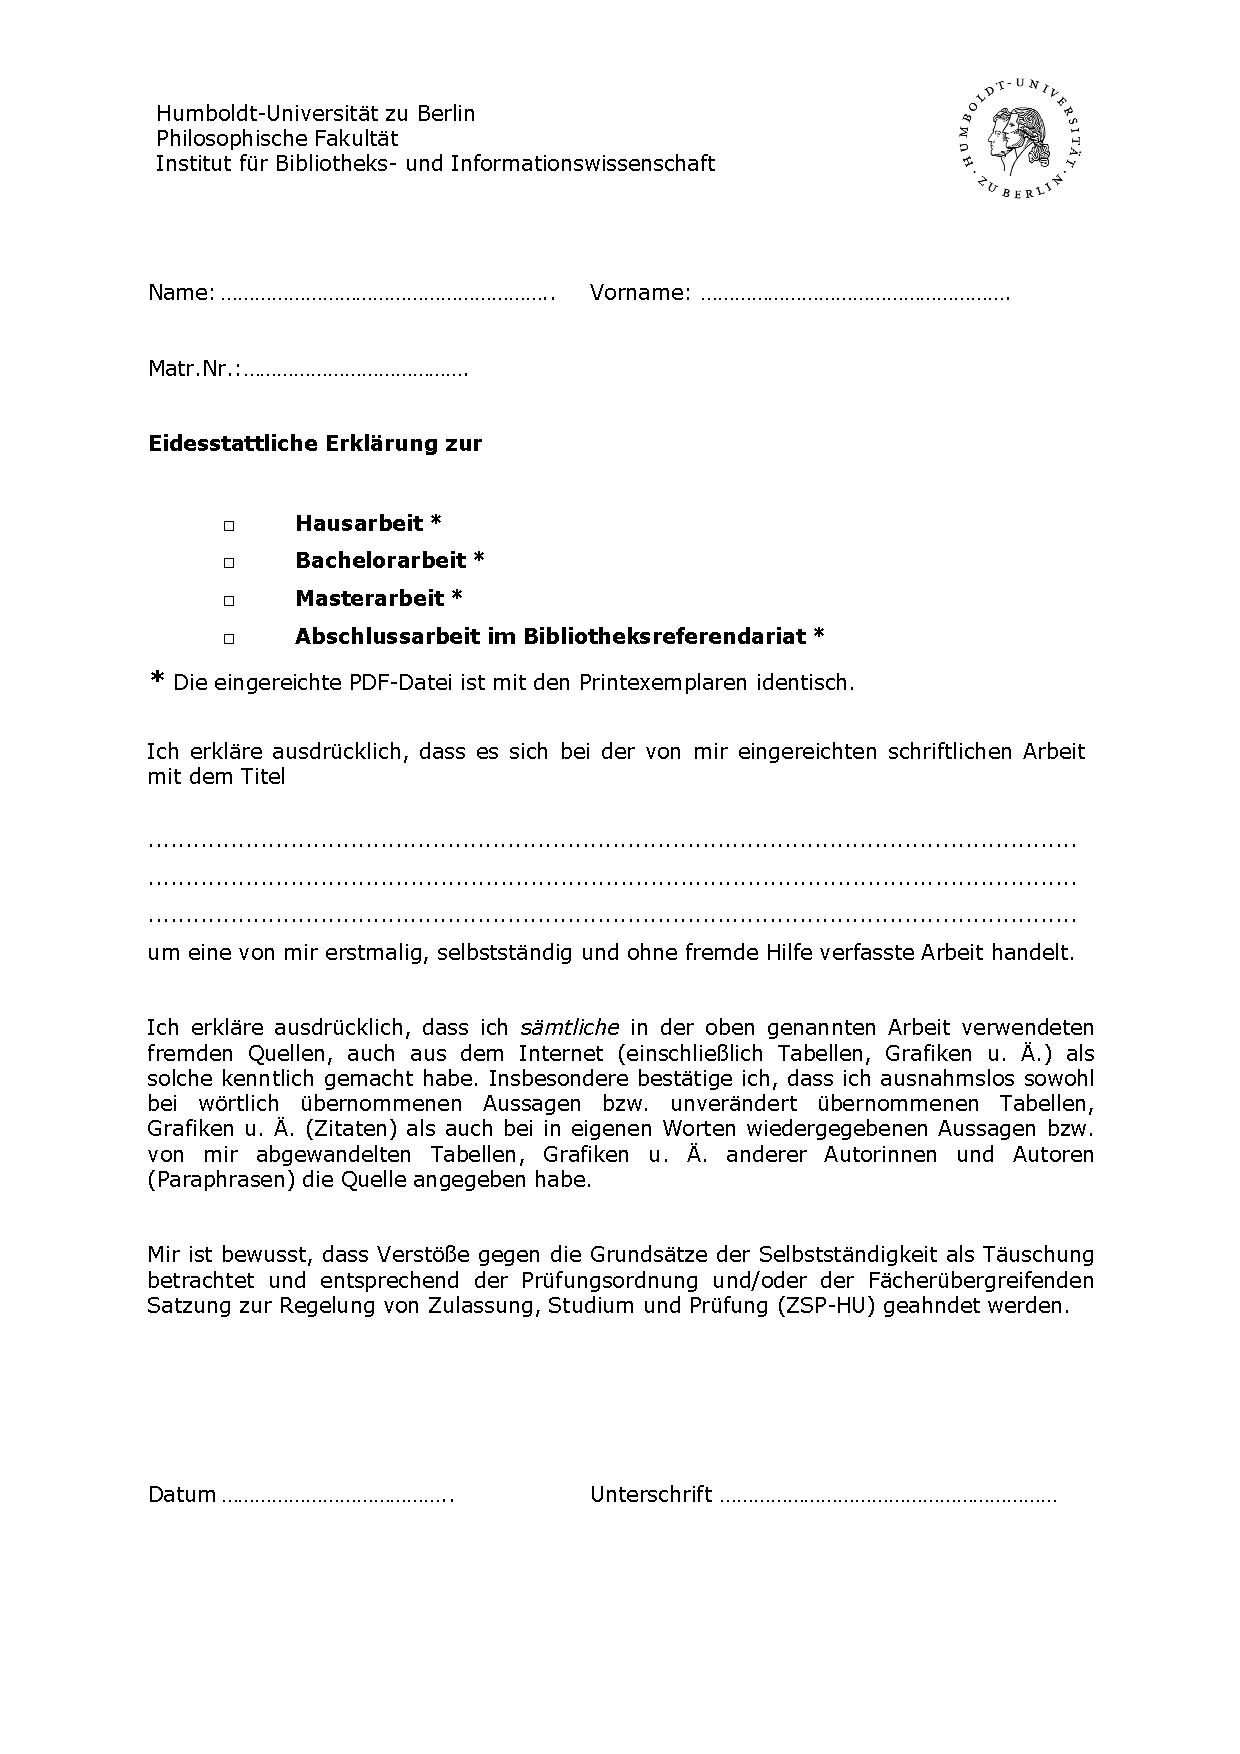
\includepdf[pages=-]{matter/backmatter/selbststaendigkeitserklaerung.pdf}
\end{document}
